% Webinar 7 of the Idiot Brain series (Armenian): chapter 7, "Group hug!" (how other people shape the brain).
% Build from the repo root (queued behind the machine-wide build lock, never run lualatex directly):
%     python 02_idiot_brain/slides/common/build_deck.py webinar07 --full     (~10-17 min)
%     python 02_idiot_brain/slides/common/build_deck.py webinar07 --parts 02 (one part, one pass)
% Needs the shared art first: uv run 02_idiot_brain/slides/common/build_art.py
% Speaker notes: NOTES.md (by frame number and title). ~95 min talk incl. a 5 min break.
\documentclass[aspectratio=169,11pt]{beamer}
% =====================================================================
%  The Idiot Brain webinars - shared Beamer preamble (the banner look)
% ---------------------------------------------------------------------
%  Usage (in slides/webinarNN/webinarNN.tex):
%      \documentclass[aspectratio=169,11pt]{beamer}
%      % =====================================================================
%  The Idiot Brain webinars - shared Beamer preamble (the banner look)
% ---------------------------------------------------------------------
%  Usage (in slides/webinarNN/webinarNN.tex):
%      \documentclass[aspectratio=169,11pt]{beamer}
%      % =====================================================================
%  The Idiot Brain webinars - shared Beamer preamble (the banner look)
% ---------------------------------------------------------------------
%  Usage (in slides/webinarNN/webinarNN.tex):
%      \documentclass[aspectratio=169,11pt]{beamer}
%      \input{../common/preamble.tex}
%  Build from the deck folder:  latexmk -lualatex -outdir=build webinarNN.tex
%  Art (emoji, mascot moods, title banner) comes from common/build_art.py.
%
%  All styling lives here, so decks only hold content. Palette and fonts
%  are the banner's (banner/build_banner.py): plum text on cream, pastel
%  accents, Mardoto for text, Glazz for big titles, Twemoji icons and
%  the pink brain mascot (DECISIONS.md #4-#6).
% =====================================================================

% ---------------------------------------------------------------------
% Fonts (LuaLaTeX + fontspec), shared with the banner
% ---------------------------------------------------------------------
\usepackage{fontspec}
\tracinglostchars=3 % a glyph missing from a font stops the build instead of printing nothing
\defaultfontfeatures{Ligatures=TeX}
\def\idiotfontdir{../../banner/assets/fonts/}
\setsansfont{Mardoto}[Path=\idiotfontdir, Extension=.ttf, UprightFont=*-Regular, BoldFont=*-Bold]
\setmainfont{Mardoto}[Path=\idiotfontdir, Extension=.ttf, UprightFont=*-Regular, BoldFont=*-Bold]
\newfontfamily\mediumfont{Mardoto-Medium}[Path=\idiotfontdir, Extension=.ttf]
\newfontfamily\blackfont{Mardoto-Black}[Path=\idiotfontdir, Extension=.ttf]
\newfontfamily\titlefont{GlazzArm-Regular}[Path=\idiotfontdir, Extension=.ttf] % Armenian letters only
\newfontfamily\handfont{Ink Free} % Windows font with Armenian; speech bubbles only
% Mardoto has no italic: emphasis is medium weight in the accent colour instead.
\renewcommand{\emph}[1]{{\mediumfont\color{plum}#1}}
% No hyphenation: split words are hard to read on a shared screen.
\hyphenpenalty=10000
\exhyphenpenalty=10000

% ---------------------------------------------------------------------
% Packages
% ---------------------------------------------------------------------
\usepackage{graphicx}
\usepackage{booktabs}
\usepackage[most]{tcolorbox}
\usepackage{tikz}
\usetikzlibrary{arrows.meta, positioning, calc, shapes.geometric, shapes.callouts, shapes.misc,
  decorations.pathmorphing, decorations.pathreplacing, backgrounds, fit, patterns.meta}
\usepackage{pgfplots}
\pgfplotsset{compat=1.18}
\usepgfplotslibrary{fillbetween}
\graphicspath{{../common/art/}{images/}}

% ---------------------------------------------------------------------
% Colours: the banner palette. Charts with 3+ series use the Armenian
% flag colours (amRed / amBlue / amOrange).
% ---------------------------------------------------------------------
\definecolor{plum}{HTML}{4A2340}
\definecolor{brainpink}{HTML}{F7A8C4}
\definecolor{fold}{HTML}{E57FA6}
\definecolor{cream}{HTML}{FFF6EC}
\definecolor{cardwhite}{HTML}{FFFDF9}
\definecolor{peach}{HTML}{FFD9C2}
\definecolor{lavender}{HTML}{D9C8F5}
\definecolor{mint}{HTML}{B5E8D5}
\definecolor{butter}{HTML}{FFE8A3}
\definecolor{blush}{HTML}{FF8FA8}
\definecolor{amRed}{HTML}{D90012}
\definecolor{amBlue}{HTML}{0033A0}
\definecolor{amOrange}{HTML}{F2A800}
% darker partners for text on cream
\colorlet{mintdark}{mint!45!black!80!green}
\definecolor{mintdark}{HTML}{2E7D62}
\definecolor{lavenderdark}{HTML}{5B3FA0}
\definecolor{peachdark}{HTML}{B5532A}
\definecolor{pinkdark}{HTML}{C2185B}
% names used by the figure files
\colorlet{ink}{plum}
\colorlet{paper}{cream}
\colorlet{mist}{lavender!40!cream}
\definecolor{night}{HTML}{2B2150}
\colorlet{softgray}{plum!60!cream}
% accent of the current part; \partaccent{<colour>} switches it
\colorlet{accent}{butter}
\newcommand{\partaccent}[1]{\colorlet{accent}{#1}}

% ---------------------------------------------------------------------
% Art: \emoji, \mascot (pages of common/art/*.pdf, see build_art.py)
% ---------------------------------------------------------------------
\makeatletter
\newcommand{\artpage}[3]{\expandafter\def\csname idiot@art@#1@#2\endcsname{#3}}
\input{../common/art/art_index.tex}
\newcommand{\idiot@art}[3]{% kind, name, size options
  \ifcsname idiot@art@#1@#2\endcsname
    \includegraphics[#3, page=\csname idiot@art@#1@#2\endcsname]{#1.pdf}%
  \else
    \PackageError{idiot}{Unknown #1 '#2'; add it to build_art.py and rebuild the art}{}%
  \fi}
% \emoji[<height>]{name}: inline icon, sits on the text baseline like a letter
\newcommand{\emoji}[2][1.15em]{\raisebox{-0.2em}{\idiot@art{emoji}{#2}{height=#1}}}
% \bigemoji[<height>]{name}: no baseline shift, for TikZ nodes and big pictures
\newcommand{\bigemoji}[2][1.5cm]{\idiot@art{emoji}{#2}{height=#1}}
% \mascot[<width>]{mood}: panic, happy, scared, sleepy, sick, confused, smug, hungry, thinking
\newcommand{\mascot}[2][2.6cm]{\idiot@art{mascot}{#2}{width=#1}}
\makeatother
% the older figure files place the mascot with \pic{noggin=<mood>}
\tikzset{pics/noggin/.style={code={\node[inner sep=0, transform shape] {\mascot[2.7cm]{#1}};}}}

% ---------------------------------------------------------------------
% Beamer look
% ---------------------------------------------------------------------
\setbeamertemplate{navigation symbols}{}
\setbeamercolor{normal text}{fg=plum, bg=cream}
\setbeamercolor{structure}{fg=plum}
\setbeamercolor{alerted text}{fg=pinkdark}
\setbeamerfont{alerted text}{series=\bfseries}
\setbeamercolor{frametitle}{fg=plum}
\setbeamersize{text margin left=9mm, text margin right=9mm}
\setbeamertemplate{frame begin}{\raggedright} % justified Armenian leaves big gaps

% cream paper with the banner's faint dot grid
\setbeamertemplate{background}{%
  \begin{tikzpicture}
    \fill[cream] (0,0) rectangle (\paperwidth,\paperheight);
    \fill[pattern={Dots[distance=4.4mm, radius=0.28mm]}, pattern color=plum!9!cream]
      (0,0) rectangle (\paperwidth,\paperheight);
  \end{tikzpicture}}

% topic pill, top right of every frame: set by \topic (emoji + short name)
\def\idiottopicemoji{}
\def\idiottopicname{}
\newcommand{\idiotpill}[3][cardwhite]{% fill, emoji, text
  \tikz[baseline=(p.base)]{\node[fill=#1, draw=plum, line width=0.7pt, rounded corners=2.6mm,
      inner xsep=2.2mm, inner ysep=1.1mm, font=\mediumfont\footnotesize, text=plum] (p)
      {\ifx\relax#2\relax\else\emoji[1.05em]{#2}\hspace{1.2mm}\fi#3};
    \begin{scope}[on background layer]
      \fill[plum, rounded corners=2.6mm] ([xshift=0.7mm, yshift=-0.7mm]p.south west) rectangle ([xshift=0.7mm, yshift=-0.7mm]p.north east);
    \end{scope}}}
% \chip{emoji}{text}: inline sticker label, same as the banner's topic chips
\newcommand{\chip}[3][cardwhite]{\idiotpill[#1]{#2}{#3}}

\setbeamertemplate{frametitle}{%
  \vskip 3.5mm
  \begin{minipage}[t]{0.66\paperwidth}
    \raggedright{\blackfont\fontsize{17.5}{20.5}\selectfont\insertframetitle}\par
    \vskip 1.3mm
    \tikz\fill[accent, rounded corners=0.6mm] (0,0) rectangle (1.5cm,1.1mm);
  \end{minipage}%
  \hfill
  \ifx\idiottopicname\empty\else
    \raisebox{-1mm}{\idiotpill{\idiottopicemoji}{\idiottopicname}}%
  \fi
  \vskip 1mm}

\setbeamertemplate{footline}{%
  \hbox to \paperwidth{\hskip 9mm
    {\mediumfont\fontsize{7}{8}\selectfont\color{plum!55!cream}Ապուշ ուղեղը · \insertshorttitle}\hfill
    {\blackfont\fontsize{8}{9}\selectfont\color{plum!70!cream}\insertframenumber}\hskip 9mm}
  \vskip 3mm}

\setbeamertemplate{itemize item}{\tikz[baseline=-0.65ex]\draw[plum, fill=accent, line width=0.6pt] (0,0) circle (0.95mm);}
\setbeamertemplate{itemize subitem}{\tikz[baseline=-0.65ex]\fill[plum!70] (0,0) circle (0.6mm);}
\setbeamertemplate{enumerate item}{\tikz[baseline=(n.base)]\node[fill=accent, draw=plum, line width=0.6pt,
  circle, inner sep=0.5mm, minimum size=4.2mm, font=\blackfont\scriptsize] (n) {\insertenumlabel};}
\setlength{\leftmargini}{5mm}
\setbeamertemplate{itemize/enumerate body begin}{\setlength{\itemsep}{1.6mm}}
\setbeamertemplate{itemize/enumerate subbody begin}{\setlength{\itemsep}{0.6mm}\small}

% ---------------------------------------------------------------------
% Structure: parts (full-colour openers) and topics (book sections)
% ---------------------------------------------------------------------
% \topic{<emoji>}{<short name>}: starts a book section; the pill shows on every following frame
\newcommand{\topic}[2]{\subsection{#2}\gdef\idiottopicemoji{#1}\gdef\idiottopicname{#2}}
\newcommand{\notopic}{\gdef\idiottopicemoji{}\gdef\idiottopicname{}}

% \partopener{<label>}{<title>}{<subtitle>}{<mood>}{<colour>}
\newcommand{\partopener}[5]{%
  \section{#2}\notopic\partaccent{#5}%
  \begin{frame}[plain]
    \begin{tikzpicture}[remember picture, overlay]
      \fill[#5] (current page.south west) rectangle (current page.north east);
      \fill[pattern={Dots[distance=4.4mm, radius=0.28mm]}, pattern color=plum!12!#5]
        (current page.south west) rectangle (current page.north east);
      \fill[cardwhite, opacity=0.45] ([xshift=-3.3cm, yshift=-0.2cm]current page.east) circle (3.1cm);
      \node[anchor=north west, inner sep=0] at ([xshift=10mm, yshift=-12mm]current page.north west)
        {\idiotpill{}{#1}};
      \node[anchor=west, text=plum, align=left, text width=9.2cm, inner sep=0]
        (t) at ([xshift=10mm, yshift=5mm]current page.west)
        {\titlefont\fontsize{38}{40}\selectfont #2};
      \node[anchor=north west, text=plum, text width=9.2cm, inner sep=0, align=left]
        at ([yshift=-5mm]t.south west) {\mediumfont\large #3};
      \node at ([xshift=-3.3cm, yshift=-0.2cm]current page.east) {\mascot[4.6cm]{#4}};
    \end{tikzpicture}
  \end{frame}}

% \topicopener{<emoji>}{<short name>}{<book's section title>}{<what it is about>}{<mood>}
\newcommand{\topicopener}[5]{%
  \topic{#1}{#2}%
  \begin{frame}[plain]
    \begin{tikzpicture}[remember picture, overlay]
      \fill[accent!55!cream] (current page.south west) rectangle (current page.north east);
      \fill[pattern={Dots[distance=4.4mm, radius=0.28mm]}, pattern color=plum!10!accent!55!cream]
        (current page.south west) rectangle (current page.north east);
      \node[anchor=north west, inner sep=0] at ([xshift=10mm, yshift=-12mm]current page.north west)
        {\idiotpill{#1}{#2}};
      \node[anchor=west, text=plum, text width=9.6cm, align=left, inner sep=0]
        (t) at ([xshift=10mm, yshift=6mm]current page.west)
        {\blackfont\fontsize{24}{28}\selectfont «#3»};
      \node[anchor=north west, text=plum, text width=9.6cm, align=left, inner sep=0]
        at ([yshift=-4mm]t.south west) {\mediumfont\large #4};
      \node at ([xshift=-3.0cm, yshift=-0.4cm]current page.east) {\mascot[4.2cm]{#5}};
      \node[rotate=-12] at ([xshift=-1.4cm, yshift=2.3cm]current page.east) {\bigemoji[1.5cm]{#1}};
    \end{tikzpicture}
  \end{frame}}

% ---------------------------------------------------------------------
% Boxes (sticker style: plum outline + hard plum shadow, like the banner)
% ---------------------------------------------------------------------
\tcbset{
  sticker/.style={enhanced, arc=3mm, boxrule=0.9pt, colframe=plum, colback=cardwhite, halign=left,
    left=3mm, right=3mm, top=2mm, bottom=2mm, fontupper=\normalsize, coltext=plum,
    shadow={1.1mm}{-1.1mm}{0mm}{fill=plum}},
  tagged/.style={sticker, colback=#1!45!cream, colbacktitle=#1, coltitle=plum,
    fonttitle=\blackfont\footnotesize, top=3mm,
    attach boxed title to top left={xshift=4mm, yshift*=-2.4mm},
    boxed title style={arc=2.2mm, boxrule=0.9pt, colframe=plum, left=1.5mm, right=1.5mm, top=0.6mm, bottom=0.6mm}},
}
\newtcolorbox{card}[1][]{sticker, #1}
\newtcolorbox{tryit}[1][]{tagged=mint, title={\emoji[1em]{testtube}\ Փորձիր հիմա}, #1}
\newtcolorbox{poll}[1][]{tagged=butter, title={\emoji[1em]{hand}\ Հարցում}, #1}
\newtcolorbox{chatbox}[1][]{tagged=lavender, title={\emoji[1em]{speech}\ Գրիր չաթում}, #1}
\newtcolorbox{scienceupdate}[1][]{tagged=peach, fontupper=\small, title={\emoji[1em]{microscope}\ Գիտությունն այսօր}, #1}
\newtcolorbox{bookquote}[1][]{sticker, colback=cardwhite, fontupper=\mediumfont, left=4mm,
  borderline west={1.4mm}{0pt}{accent},
  before upper={{\blackfont\footnotesize\emoji[1em]{book}\ Բըրնեթը գրում է}\par\smallskip}, #1}

% Brain.exe-style popup window: \begin{popup}{<window title>} ... \end{popup}
\newcommand{\winbuttons}{%
  \tikz[baseline=-0.6ex, line width=0.6pt]{
    \foreach \i/\f in {0/cardwhite, 1/cardwhite, 2/blush}{
      \filldraw[fill=\f, draw=plum, rounded corners=0.6mm] (\i*4.3mm,-1.6mm) rectangle ++(3.3mm,3.3mm);}
    \draw[plum] (0.8mm,-0.8mm) -- (2.5mm,-0.8mm);
    \draw[plum] (5.1mm,-0.8mm) rectangle (6.8mm,0.9mm);
    \draw[plum] (9.4mm,-0.9mm) -- (11.1mm,0.8mm) (9.4mm,0.8mm) -- (11.1mm,-0.9mm);}}
\newtcolorbox{popup}[2][]{sticker, colback=cardwhite, colbacktitle=brainpink, coltitle=plum,
  fonttitle=\blackfont\small, title={\emoji[1.1em]{warning}\hspace{1.5mm}#2\hfill\winbuttons},
  titlerule=0.9pt, toptitle=0.8mm, bottomtitle=0.8mm, #1}

% Myth or fact: \mythorfact{<statement>}{<verdict>}{<colour>}{<explanation>}; verdict shows on slide 2
\newcommand{\mythorfact}[4]{%
  \begin{center}
  \begin{tikzpicture}
    \node[draw=plum, line width=0.9pt, fill=cardwhite, rounded corners=4mm, inner xsep=8mm, inner ysep=6mm,
          text width=10cm, align=center, font=\blackfont\Large, text=plum] (mf) {«#1»};
    \begin{scope}[on background layer]
      \fill[plum, rounded corners=4mm] ([xshift=1.2mm, yshift=-1.2mm]mf.south west) rectangle ([xshift=1.2mm, yshift=-1.2mm]mf.north east);
    \end{scope}
    \node[anchor=west] at ([xshift=6mm]mf.north west) {\idiotpill[butter]{question}{Առասպել, թե՞ փաստ}};
    \onslide<2->{\node[draw=#3, text=#3, line width=2pt, rounded corners=2mm, rotate=-10, font=\blackfont\LARGE,
      inner sep=4pt, fill=cardwhite] at ([xshift=-8mm, yshift=1mm]mf.south east) {#2};}
  \end{tikzpicture}
  \end{center}
  \onslide<2->{#4}}

% Big question with the confused mascot: \bigquestion{<question>}{<small line>}
\newcommand{\bigquestion}[2]{%
  \vfill
  \begin{center}
  \begin{tikzpicture}
    \node[text width=9.6cm, align=center, font=\blackfont\fontsize{24}{29}\selectfont, text=plum] (q) {#1};
    \node[below=4mm of q, text width=9.6cm, align=center, font=\mediumfont\large, text=softgray] {#2};
    \node[anchor=east] at ([xshift=-2mm]q.west) {\mascot[2.6cm]{confused}};
  \end{tikzpicture}
  \end{center}
  \vfill}

% Small source line at the bottom of a frame: \source{Loftus & Palmer, 1974}
\newcommand{\source}[1]{%
  \begin{tikzpicture}[remember picture, overlay]
    \node[anchor=south east, font=\fontsize{6.5}{7.5}\selectfont, text=plum!60!cream, inner sep=0]
      at ([xshift=-17mm, yshift=3.4mm]current page.south east) {Աղբյուր՝ #1};
  \end{tikzpicture}}

% Speech bubbles (handwritten) and the overlay helper for TikZ:
% \node[visible on=<2->] ... keeps the layout but hides the node until slide 2.
\tikzset{
  say/.style={rectangle callout, draw=plum, line width=0.8pt, fill=cardwhite, rounded corners=3pt,
    inner sep=4pt, align=center, font=\handfont\normalsize, text=plum},
  think/.style={cloud callout, cloud puffs=12, draw=plum, line width=0.8pt, fill=cardwhite,
    inner sep=2pt, align=center, font=\handfont\normalsize, text=plum},
  % boxes for diagrams drawn directly in a frame: a style with #1 cannot be defined inside a frame body
  flow/.style={draw=plum, line width=0.8pt, fill=cardwhite, rounded corners=2mm, align=center,
    font=\small, text=plum, inner sep=4pt, text width=#1},
  flow/.default=3cm,
  chatmsg/.style={draw=plum, line width=0.8pt, rounded corners=3mm, inner sep=6pt, text width=#1,
    align=left, font=\small, text=plum},
  chatmsg/.default=7cm,
  invisible/.style={opacity=0, text opacity=0},
  visible on/.style={alt={#1{}{invisible}}},
  alt/.code args={<#1>#2#3}{\alt<#1>{\pgfkeysalso{#2}}{\pgfkeysalso{#3}}},
}

%  Build from the deck folder:  latexmk -lualatex -outdir=build webinarNN.tex
%  Art (emoji, mascot moods, title banner) comes from common/build_art.py.
%
%  All styling lives here, so decks only hold content. Palette and fonts
%  are the banner's (banner/build_banner.py): plum text on cream, pastel
%  accents, Mardoto for text, Glazz for big titles, Twemoji icons and
%  the pink brain mascot (DECISIONS.md #4-#6).
% =====================================================================

% ---------------------------------------------------------------------
% Fonts (LuaLaTeX + fontspec), shared with the banner
% ---------------------------------------------------------------------
\usepackage{fontspec}
\tracinglostchars=3 % a glyph missing from a font stops the build instead of printing nothing
\defaultfontfeatures{Ligatures=TeX}
\def\idiotfontdir{../../banner/assets/fonts/}
\setsansfont{Mardoto}[Path=\idiotfontdir, Extension=.ttf, UprightFont=*-Regular, BoldFont=*-Bold]
\setmainfont{Mardoto}[Path=\idiotfontdir, Extension=.ttf, UprightFont=*-Regular, BoldFont=*-Bold]
\newfontfamily\mediumfont{Mardoto-Medium}[Path=\idiotfontdir, Extension=.ttf]
\newfontfamily\blackfont{Mardoto-Black}[Path=\idiotfontdir, Extension=.ttf]
\newfontfamily\titlefont{GlazzArm-Regular}[Path=\idiotfontdir, Extension=.ttf] % Armenian letters only
\newfontfamily\handfont{Ink Free} % Windows font with Armenian; speech bubbles only
% Mardoto has no italic: emphasis is medium weight in the accent colour instead.
\renewcommand{\emph}[1]{{\mediumfont\color{plum}#1}}
% No hyphenation: split words are hard to read on a shared screen.
\hyphenpenalty=10000
\exhyphenpenalty=10000

% ---------------------------------------------------------------------
% Packages
% ---------------------------------------------------------------------
\usepackage{graphicx}
\usepackage{booktabs}
\usepackage[most]{tcolorbox}
\usepackage{tikz}
\usetikzlibrary{arrows.meta, positioning, calc, shapes.geometric, shapes.callouts, shapes.misc,
  decorations.pathmorphing, decorations.pathreplacing, backgrounds, fit, patterns.meta}
\usepackage{pgfplots}
\pgfplotsset{compat=1.18}
\usepgfplotslibrary{fillbetween}
\graphicspath{{../common/art/}{images/}}

% ---------------------------------------------------------------------
% Colours: the banner palette. Charts with 3+ series use the Armenian
% flag colours (amRed / amBlue / amOrange).
% ---------------------------------------------------------------------
\definecolor{plum}{HTML}{4A2340}
\definecolor{brainpink}{HTML}{F7A8C4}
\definecolor{fold}{HTML}{E57FA6}
\definecolor{cream}{HTML}{FFF6EC}
\definecolor{cardwhite}{HTML}{FFFDF9}
\definecolor{peach}{HTML}{FFD9C2}
\definecolor{lavender}{HTML}{D9C8F5}
\definecolor{mint}{HTML}{B5E8D5}
\definecolor{butter}{HTML}{FFE8A3}
\definecolor{blush}{HTML}{FF8FA8}
\definecolor{amRed}{HTML}{D90012}
\definecolor{amBlue}{HTML}{0033A0}
\definecolor{amOrange}{HTML}{F2A800}
% darker partners for text on cream
\colorlet{mintdark}{mint!45!black!80!green}
\definecolor{mintdark}{HTML}{2E7D62}
\definecolor{lavenderdark}{HTML}{5B3FA0}
\definecolor{peachdark}{HTML}{B5532A}
\definecolor{pinkdark}{HTML}{C2185B}
% names used by the figure files
\colorlet{ink}{plum}
\colorlet{paper}{cream}
\colorlet{mist}{lavender!40!cream}
\definecolor{night}{HTML}{2B2150}
\colorlet{softgray}{plum!60!cream}
% accent of the current part; \partaccent{<colour>} switches it
\colorlet{accent}{butter}
\newcommand{\partaccent}[1]{\colorlet{accent}{#1}}

% ---------------------------------------------------------------------
% Art: \emoji, \mascot (pages of common/art/*.pdf, see build_art.py)
% ---------------------------------------------------------------------
\makeatletter
\newcommand{\artpage}[3]{\expandafter\def\csname idiot@art@#1@#2\endcsname{#3}}
% generated by build_art.py - do not edit
\artpage{emoji}{brain}{1}
\artpage{emoji}{warning}{2}
\artpage{emoji}{rollercoaster}{3}
\artpage{emoji}{doughnut}{4}
\artpage{emoji}{sleeping}{5}
\artpage{emoji}{scream}{6}
\artpage{emoji}{thought}{7}
\artpage{emoji}{question}{8}
\artpage{emoji}{cyclone}{9}
\artpage{emoji}{calendar}{10}
\artpage{emoji}{clock630}{11}
\artpage{emoji}{computer}{12}
\artpage{emoji}{receipt}{13}
\artpage{emoji}{gift}{14}
\artpage{emoji}{lizard}{15}
\artpage{emoji}{boss}{16}
\artpage{emoji}{keyboard}{17}
\artpage{emoji}{wastebasket}{18}
\artpage{emoji}{batterylow}{19}
\artpage{emoji}{skull}{20}
\artpage{emoji}{car}{21}
\artpage{emoji}{ship}{22}
\artpage{emoji}{airplane}{23}
\artpage{emoji}{nauseated}{24}
\artpage{emoji}{vomit}{25}
\artpage{emoji}{eye}{26}
\artpage{emoji}{ear}{27}
\artpage{emoji}{tree}{28}
\artpage{emoji}{wave}{29}
\artpage{emoji}{book}{30}
\artpage{emoji}{walking}{31}
\artpage{emoji}{dizzy}{32}
\artpage{emoji}{cake}{33}
\artpage{emoji}{icecream}{34}
\artpage{emoji}{potato}{35}
\artpage{emoji}{apple}{36}
\artpage{emoji}{burger}{37}
\artpage{emoji}{salad}{38}
\artpage{emoji}{clock12}{39}
\artpage{emoji}{forkknife}{40}
\artpage{emoji}{pasta}{41}
\artpage{emoji}{fire}{42}
\artpage{emoji}{drool}{43}
\artpage{emoji}{pizza}{44}
\artpage{emoji}{bed}{45}
\artpage{emoji}{personbed}{46}
\artpage{emoji}{moon}{47}
\artpage{emoji}{sun}{48}
\artpage{emoji}{zzz}{49}
\artpage{emoji}{dolphin}{50}
\artpage{emoji}{jellyfish}{51}
\artpage{emoji}{rat}{52}
\artpage{emoji}{chipmunk}{53}
\artpage{emoji}{alarm}{54}
\artpage{emoji}{phone}{55}
\artpage{emoji}{ghost}{56}
\artpage{emoji}{alien}{57}
\artpage{emoji}{yawn}{58}
\artpage{emoji}{baby}{59}
\artpage{emoji}{construction}{60}
\artpage{emoji}{broom}{61}
\artpage{emoji}{thermometer}{62}
\artpage{emoji}{cold}{63}
\artpage{emoji}{monkey}{64}
\artpage{emoji}{tiger}{65}
\artpage{emoji}{axe}{66}
\artpage{emoji}{balloon}{67}
\artpage{emoji}{heart}{68}
\artpage{emoji}{anatomicalheart}{69}
\artpage{emoji}{lungs}{70}
\artpage{emoji}{sweat}{71}
\artpage{emoji}{eyes}{72}
\artpage{emoji}{butterfly}{73}
\artpage{emoji}{runner}{74}
\artpage{emoji}{boxing}{75}
\artpage{emoji}{station}{76}
\artpage{emoji}{taxi}{77}
\artpage{emoji}{bell}{78}
\artpage{emoji}{couch}{79}
\artpage{emoji}{muscle}{80}
\artpage{emoji}{toilet}{81}
\artpage{emoji}{floppy}{82}
\artpage{emoji}{door}{83}
\artpage{emoji}{coffee}{84}
\artpage{emoji}{diving}{85}
\artpage{emoji}{wine}{86}
\artpage{emoji}{beer}{87}
\artpage{emoji}{dove}{88}
\artpage{emoji}{puzzle}{89}
\artpage{emoji}{fish}{90}
\artpage{emoji}{trophy}{91}
\artpage{emoji}{detective}{92}
\artpage{emoji}{judge}{93}
\artpage{emoji}{cheese}{94}
\artpage{emoji}{film}{95}
\artpage{emoji}{magnifier}{96}
\artpage{emoji}{key}{97}
\artpage{emoji}{firework}{98}
\artpage{emoji}{house}{99}
\artpage{emoji}{gloves}{100}
\artpage{emoji}{trafficlight}{101}
\artpage{emoji}{stop}{102}
\artpage{emoji}{mute}{103}
\artpage{emoji}{videogame}{104}
\artpage{emoji}{mirror}{105}
\artpage{emoji}{star}{106}
\artpage{emoji}{hospital}{107}
\artpage{emoji}{pill}{108}
\artpage{emoji}{camera}{109}
\artpage{emoji}{tv}{110}
\artpage{emoji}{crown}{111}
\artpage{emoji}{nerd}{112}
\artpage{emoji}{lock}{113}
\artpage{emoji}{musical}{114}
\artpage{emoji}{chips}{115}
\artpage{emoji}{check}{116}
\artpage{emoji}{cross}{117}
\artpage{emoji}{hand}{118}
\artpage{emoji}{wavehand}{119}
\artpage{emoji}{speech}{120}
\artpage{emoji}{pencil}{121}
\artpage{emoji}{memo}{122}
\artpage{emoji}{monocle}{123}
\artpage{emoji}{thinking}{124}
\artpage{emoji}{grin}{125}
\artpage{emoji}{sweatsmile}{126}
\artpage{emoji}{facepalm}{127}
\artpage{emoji}{popcorn}{128}
\artpage{emoji}{bulb}{129}
\artpage{emoji}{sparkles}{130}
\artpage{emoji}{party}{131}
\artpage{emoji}{chart}{132}
\artpage{emoji}{testtube}{133}
\artpage{emoji}{people}{134}
\artpage{emoji}{pin}{135}
\artpage{emoji}{hourglass}{136}
\artpage{emoji}{microscope}{137}
\artpage{emoji}{books}{138}
\artpage{emoji}{megaphone}{139}
\artpage{emoji}{student}{140}
\artpage{emoji}{zany}{141}
\artpage{emoji}{hundred}{142}
\artpage{emoji}{link}{143}
\artpage{emoji}{target}{144}
\artpage{emoji}{clover}{145}
\artpage{emoji}{ufo}{146}
\artpage{emoji}{spider}{147}
\artpage{emoji}{spiderweb}{148}
\artpage{emoji}{snake}{149}
\artpage{emoji}{microphone}{150}
\artpage{emoji}{clown}{151}
\artpage{emoji}{pumpkin}{152}
\artpage{emoji}{knife}{153}
\artpage{emoji}{bat}{154}
\artpage{emoji}{blackcat}{155}
\artpage{emoji}{crossedfingers}{156}
\artpage{emoji}{ladder}{157}
\artpage{emoji}{thumbsup}{158}
\artpage{emoji}{thumbsdown}{159}
\artpage{emoji}{rocket}{160}
\artpage{emoji}{satellite}{161}
\artpage{emoji}{newspaper}{162}
\artpage{emoji}{chocolate}{163}
\artpage{emoji}{syringe}{164}
\artpage{emoji}{dice}{165}
\artpage{emoji}{hauntedhouse}{166}
\artpage{emoji}{flushed}{167}
\artpage{emoji}{fearful}{168}
\artpage{emoji}{graduation}{169}
\artpage{emoji}{teacher}{170}
\artpage{emoji}{scientist}{171}
\artpage{emoji}{chess}{172}
\artpage{emoji}{abacus}{173}
\artpage{emoji}{ruler}{174}
\artpage{emoji}{jeans}{175}
\artpage{emoji}{glasses}{176}
\artpage{emoji}{dna}{177}
\artpage{emoji}{loudspeaker}{178}
\artpage{emoji}{speakinghead}{179}
\artpage{emoji}{seedling}{180}
\artpage{emoji}{weightlifter}{181}
\artpage{emoji}{giraffe}{182}
\artpage{emoji}{mouse}{183}
\artpage{emoji}{exploding}{184}
\artpage{emoji}{owl}{185}
\artpage{emoji}{clipboard}{186}
\artpage{emoji}{numbers}{187}
\artpage{emoji}{medal}{188}
\artpage{emoji}{rose}{189}
\artpage{emoji}{nose}{190}
\artpage{emoji}{tongue}{191}
\artpage{emoji}{yum}{192}
\artpage{emoji}{bread}{193}
\artpage{emoji}{lemon}{194}
\artpage{emoji}{chili}{195}
\artpage{emoji}{salt}{196}
\artpage{emoji}{candy}{197}
\artpage{emoji}{speaker}{198}
\artpage{emoji}{headphones}{199}
\artpage{emoji}{feather}{200}
\artpage{emoji}{gorilla}{201}
\artpage{emoji}{basketball}{202}
\artpage{emoji}{magicwand}{203}
\artpage{emoji}{tophat}{204}
\artpage{emoji}{cloud}{205}
\artpage{emoji}{plug}{206}
\artpage{emoji}{clinking}{207}
\artpage{emoji}{dog}{208}
\artpage{emoji}{rainbow}{209}
\artpage{emoji}{slightsmile}{210}
\artpage{emoji}{palette}{211}
\artpage{emoji}{masks}{212}
\artpage{emoji}{angry}{213}
\artpage{emoji}{rage}{214}
\artpage{emoji}{steam}{215}
\artpage{emoji}{bomb}{216}
\artpage{emoji}{volcano}{217}
\artpage{emoji}{angersymbol}{218}
\artpage{emoji}{crystalball}{219}
\artpage{emoji}{railway}{220}
\artpage{emoji}{worker}{221}
\artpage{emoji}{laughing}{222}
\artpage{emoji}{rofl}{223}
\artpage{emoji}{banana}{224}
\artpage{emoji}{mountain}{225}
\artpage{emoji}{moneybag}{226}
\artpage{emoji}{lightning}{227}
\artpage{emoji}{joker}{228}
\artpage{emoji}{finishflag}{229}
\artpage{emoji}{hug}{230}
\artpage{emoji}{handshake}{231}
\artpage{emoji}{lying}{232}
\artpage{emoji}{neutral}{233}
\artpage{emoji}{carrot}{234}
\artpage{emoji}{wood}{235}
\artpage{emoji}{brokenheart}{236}
\artpage{emoji}{loveletter}{237}
\artpage{emoji}{couple}{238}
\artpage{emoji}{kiss}{239}
\artpage{emoji}{cowboy}{240}
\artpage{emoji}{guitar}{241}
\artpage{emoji}{family}{242}
\artpage{emoji}{police}{243}
\artpage{emoji}{sheep}{244}
\artpage{emoji}{clapping}{245}
\artpage{emoji}{imp}{246}
\artpage{emoji}{ballot}{247}
\artpage{emoji}{smileheart}{248}
\artpage{emoji}{dollar}{249}
\artpage{emoji}{earth}{250}
\artpage{emoji}{raincloud}{251}
\artpage{emoji}{sunbehindcloud}{252}
\artpage{emoji}{pensive}{253}
\artpage{emoji}{cry}{254}
\artpage{emoji}{bandage}{255}
\artpage{emoji}{stethoscope}{256}
\artpage{emoji}{cigarette}{257}
\artpage{emoji}{slotmachine}{258}
\artpage{emoji}{siren}{259}
\artpage{emoji}{sunrise}{260}
\artpage{emoji}{healthworker}{261}
\artpage{emoji}{hearnoevil}{262}
\artpage{emoji}{anchor}{263}
\artpage{emoji}{candle}{264}
\artpage{emoji}{telephone}{265}
\artpage{emoji}{battery}{266}
\artpage{emoji}{weary}{267}
\artpage{emoji}{lotus}{268}
\artpage{mascot}{panic}{1}
\artpage{mascot}{happy}{2}
\artpage{mascot}{scared}{3}
\artpage{mascot}{sleepy}{4}
\artpage{mascot}{sick}{5}
\artpage{mascot}{confused}{6}
\artpage{mascot}{smug}{7}
\artpage{mascot}{hungry}{8}
\artpage{mascot}{thinking}{9}
\artpage{mascot}{sad}{10}
\artpage{mascot}{angry}{11}

\newcommand{\idiot@art}[3]{% kind, name, size options
  \ifcsname idiot@art@#1@#2\endcsname
    \includegraphics[#3, page=\csname idiot@art@#1@#2\endcsname]{#1.pdf}%
  \else
    \PackageError{idiot}{Unknown #1 '#2'; add it to build_art.py and rebuild the art}{}%
  \fi}
% \emoji[<height>]{name}: inline icon, sits on the text baseline like a letter
\newcommand{\emoji}[2][1.15em]{\raisebox{-0.2em}{\idiot@art{emoji}{#2}{height=#1}}}
% \bigemoji[<height>]{name}: no baseline shift, for TikZ nodes and big pictures
\newcommand{\bigemoji}[2][1.5cm]{\idiot@art{emoji}{#2}{height=#1}}
% \mascot[<width>]{mood}: panic, happy, scared, sleepy, sick, confused, smug, hungry, thinking
\newcommand{\mascot}[2][2.6cm]{\idiot@art{mascot}{#2}{width=#1}}
\makeatother
% the older figure files place the mascot with \pic{noggin=<mood>}
\tikzset{pics/noggin/.style={code={\node[inner sep=0, transform shape] {\mascot[2.7cm]{#1}};}}}

% ---------------------------------------------------------------------
% Beamer look
% ---------------------------------------------------------------------
\setbeamertemplate{navigation symbols}{}
\setbeamercolor{normal text}{fg=plum, bg=cream}
\setbeamercolor{structure}{fg=plum}
\setbeamercolor{alerted text}{fg=pinkdark}
\setbeamerfont{alerted text}{series=\bfseries}
\setbeamercolor{frametitle}{fg=plum}
\setbeamersize{text margin left=9mm, text margin right=9mm}
\setbeamertemplate{frame begin}{\raggedright} % justified Armenian leaves big gaps

% cream paper with the banner's faint dot grid
\setbeamertemplate{background}{%
  \begin{tikzpicture}
    \fill[cream] (0,0) rectangle (\paperwidth,\paperheight);
    \fill[pattern={Dots[distance=4.4mm, radius=0.28mm]}, pattern color=plum!9!cream]
      (0,0) rectangle (\paperwidth,\paperheight);
  \end{tikzpicture}}

% topic pill, top right of every frame: set by \topic (emoji + short name)
\def\idiottopicemoji{}
\def\idiottopicname{}
\newcommand{\idiotpill}[3][cardwhite]{% fill, emoji, text
  \tikz[baseline=(p.base)]{\node[fill=#1, draw=plum, line width=0.7pt, rounded corners=2.6mm,
      inner xsep=2.2mm, inner ysep=1.1mm, font=\mediumfont\footnotesize, text=plum] (p)
      {\ifx\relax#2\relax\else\emoji[1.05em]{#2}\hspace{1.2mm}\fi#3};
    \begin{scope}[on background layer]
      \fill[plum, rounded corners=2.6mm] ([xshift=0.7mm, yshift=-0.7mm]p.south west) rectangle ([xshift=0.7mm, yshift=-0.7mm]p.north east);
    \end{scope}}}
% \chip{emoji}{text}: inline sticker label, same as the banner's topic chips
\newcommand{\chip}[3][cardwhite]{\idiotpill[#1]{#2}{#3}}

\setbeamertemplate{frametitle}{%
  \vskip 3.5mm
  \begin{minipage}[t]{0.66\paperwidth}
    \raggedright{\blackfont\fontsize{17.5}{20.5}\selectfont\insertframetitle}\par
    \vskip 1.3mm
    \tikz\fill[accent, rounded corners=0.6mm] (0,0) rectangle (1.5cm,1.1mm);
  \end{minipage}%
  \hfill
  \ifx\idiottopicname\empty\else
    \raisebox{-1mm}{\idiotpill{\idiottopicemoji}{\idiottopicname}}%
  \fi
  \vskip 1mm}

\setbeamertemplate{footline}{%
  \hbox to \paperwidth{\hskip 9mm
    {\mediumfont\fontsize{7}{8}\selectfont\color{plum!55!cream}Ապուշ ուղեղը · \insertshorttitle}\hfill
    {\blackfont\fontsize{8}{9}\selectfont\color{plum!70!cream}\insertframenumber}\hskip 9mm}
  \vskip 3mm}

\setbeamertemplate{itemize item}{\tikz[baseline=-0.65ex]\draw[plum, fill=accent, line width=0.6pt] (0,0) circle (0.95mm);}
\setbeamertemplate{itemize subitem}{\tikz[baseline=-0.65ex]\fill[plum!70] (0,0) circle (0.6mm);}
\setbeamertemplate{enumerate item}{\tikz[baseline=(n.base)]\node[fill=accent, draw=plum, line width=0.6pt,
  circle, inner sep=0.5mm, minimum size=4.2mm, font=\blackfont\scriptsize] (n) {\insertenumlabel};}
\setlength{\leftmargini}{5mm}
\setbeamertemplate{itemize/enumerate body begin}{\setlength{\itemsep}{1.6mm}}
\setbeamertemplate{itemize/enumerate subbody begin}{\setlength{\itemsep}{0.6mm}\small}

% ---------------------------------------------------------------------
% Structure: parts (full-colour openers) and topics (book sections)
% ---------------------------------------------------------------------
% \topic{<emoji>}{<short name>}: starts a book section; the pill shows on every following frame
\newcommand{\topic}[2]{\subsection{#2}\gdef\idiottopicemoji{#1}\gdef\idiottopicname{#2}}
\newcommand{\notopic}{\gdef\idiottopicemoji{}\gdef\idiottopicname{}}

% \partopener{<label>}{<title>}{<subtitle>}{<mood>}{<colour>}
\newcommand{\partopener}[5]{%
  \section{#2}\notopic\partaccent{#5}%
  \begin{frame}[plain]
    \begin{tikzpicture}[remember picture, overlay]
      \fill[#5] (current page.south west) rectangle (current page.north east);
      \fill[pattern={Dots[distance=4.4mm, radius=0.28mm]}, pattern color=plum!12!#5]
        (current page.south west) rectangle (current page.north east);
      \fill[cardwhite, opacity=0.45] ([xshift=-3.3cm, yshift=-0.2cm]current page.east) circle (3.1cm);
      \node[anchor=north west, inner sep=0] at ([xshift=10mm, yshift=-12mm]current page.north west)
        {\idiotpill{}{#1}};
      \node[anchor=west, text=plum, align=left, text width=9.2cm, inner sep=0]
        (t) at ([xshift=10mm, yshift=5mm]current page.west)
        {\titlefont\fontsize{38}{40}\selectfont #2};
      \node[anchor=north west, text=plum, text width=9.2cm, inner sep=0, align=left]
        at ([yshift=-5mm]t.south west) {\mediumfont\large #3};
      \node at ([xshift=-3.3cm, yshift=-0.2cm]current page.east) {\mascot[4.6cm]{#4}};
    \end{tikzpicture}
  \end{frame}}

% \topicopener{<emoji>}{<short name>}{<book's section title>}{<what it is about>}{<mood>}
\newcommand{\topicopener}[5]{%
  \topic{#1}{#2}%
  \begin{frame}[plain]
    \begin{tikzpicture}[remember picture, overlay]
      \fill[accent!55!cream] (current page.south west) rectangle (current page.north east);
      \fill[pattern={Dots[distance=4.4mm, radius=0.28mm]}, pattern color=plum!10!accent!55!cream]
        (current page.south west) rectangle (current page.north east);
      \node[anchor=north west, inner sep=0] at ([xshift=10mm, yshift=-12mm]current page.north west)
        {\idiotpill{#1}{#2}};
      \node[anchor=west, text=plum, text width=9.6cm, align=left, inner sep=0]
        (t) at ([xshift=10mm, yshift=6mm]current page.west)
        {\blackfont\fontsize{24}{28}\selectfont «#3»};
      \node[anchor=north west, text=plum, text width=9.6cm, align=left, inner sep=0]
        at ([yshift=-4mm]t.south west) {\mediumfont\large #4};
      \node at ([xshift=-3.0cm, yshift=-0.4cm]current page.east) {\mascot[4.2cm]{#5}};
      \node[rotate=-12] at ([xshift=-1.4cm, yshift=2.3cm]current page.east) {\bigemoji[1.5cm]{#1}};
    \end{tikzpicture}
  \end{frame}}

% ---------------------------------------------------------------------
% Boxes (sticker style: plum outline + hard plum shadow, like the banner)
% ---------------------------------------------------------------------
\tcbset{
  sticker/.style={enhanced, arc=3mm, boxrule=0.9pt, colframe=plum, colback=cardwhite, halign=left,
    left=3mm, right=3mm, top=2mm, bottom=2mm, fontupper=\normalsize, coltext=plum,
    shadow={1.1mm}{-1.1mm}{0mm}{fill=plum}},
  tagged/.style={sticker, colback=#1!45!cream, colbacktitle=#1, coltitle=plum,
    fonttitle=\blackfont\footnotesize, top=3mm,
    attach boxed title to top left={xshift=4mm, yshift*=-2.4mm},
    boxed title style={arc=2.2mm, boxrule=0.9pt, colframe=plum, left=1.5mm, right=1.5mm, top=0.6mm, bottom=0.6mm}},
}
\newtcolorbox{card}[1][]{sticker, #1}
\newtcolorbox{tryit}[1][]{tagged=mint, title={\emoji[1em]{testtube}\ Փորձիր հիմա}, #1}
\newtcolorbox{poll}[1][]{tagged=butter, title={\emoji[1em]{hand}\ Հարցում}, #1}
\newtcolorbox{chatbox}[1][]{tagged=lavender, title={\emoji[1em]{speech}\ Գրիր չաթում}, #1}
\newtcolorbox{scienceupdate}[1][]{tagged=peach, fontupper=\small, title={\emoji[1em]{microscope}\ Գիտությունն այսօր}, #1}
\newtcolorbox{bookquote}[1][]{sticker, colback=cardwhite, fontupper=\mediumfont, left=4mm,
  borderline west={1.4mm}{0pt}{accent},
  before upper={{\blackfont\footnotesize\emoji[1em]{book}\ Բըրնեթը գրում է}\par\smallskip}, #1}

% Brain.exe-style popup window: \begin{popup}{<window title>} ... \end{popup}
\newcommand{\winbuttons}{%
  \tikz[baseline=-0.6ex, line width=0.6pt]{
    \foreach \i/\f in {0/cardwhite, 1/cardwhite, 2/blush}{
      \filldraw[fill=\f, draw=plum, rounded corners=0.6mm] (\i*4.3mm,-1.6mm) rectangle ++(3.3mm,3.3mm);}
    \draw[plum] (0.8mm,-0.8mm) -- (2.5mm,-0.8mm);
    \draw[plum] (5.1mm,-0.8mm) rectangle (6.8mm,0.9mm);
    \draw[plum] (9.4mm,-0.9mm) -- (11.1mm,0.8mm) (9.4mm,0.8mm) -- (11.1mm,-0.9mm);}}
\newtcolorbox{popup}[2][]{sticker, colback=cardwhite, colbacktitle=brainpink, coltitle=plum,
  fonttitle=\blackfont\small, title={\emoji[1.1em]{warning}\hspace{1.5mm}#2\hfill\winbuttons},
  titlerule=0.9pt, toptitle=0.8mm, bottomtitle=0.8mm, #1}

% Myth or fact: \mythorfact{<statement>}{<verdict>}{<colour>}{<explanation>}; verdict shows on slide 2
\newcommand{\mythorfact}[4]{%
  \begin{center}
  \begin{tikzpicture}
    \node[draw=plum, line width=0.9pt, fill=cardwhite, rounded corners=4mm, inner xsep=8mm, inner ysep=6mm,
          text width=10cm, align=center, font=\blackfont\Large, text=plum] (mf) {«#1»};
    \begin{scope}[on background layer]
      \fill[plum, rounded corners=4mm] ([xshift=1.2mm, yshift=-1.2mm]mf.south west) rectangle ([xshift=1.2mm, yshift=-1.2mm]mf.north east);
    \end{scope}
    \node[anchor=west] at ([xshift=6mm]mf.north west) {\idiotpill[butter]{question}{Առասպել, թե՞ փաստ}};
    \onslide<2->{\node[draw=#3, text=#3, line width=2pt, rounded corners=2mm, rotate=-10, font=\blackfont\LARGE,
      inner sep=4pt, fill=cardwhite] at ([xshift=-8mm, yshift=1mm]mf.south east) {#2};}
  \end{tikzpicture}
  \end{center}
  \onslide<2->{#4}}

% Big question with the confused mascot: \bigquestion{<question>}{<small line>}
\newcommand{\bigquestion}[2]{%
  \vfill
  \begin{center}
  \begin{tikzpicture}
    \node[text width=9.6cm, align=center, font=\blackfont\fontsize{24}{29}\selectfont, text=plum] (q) {#1};
    \node[below=4mm of q, text width=9.6cm, align=center, font=\mediumfont\large, text=softgray] {#2};
    \node[anchor=east] at ([xshift=-2mm]q.west) {\mascot[2.6cm]{confused}};
  \end{tikzpicture}
  \end{center}
  \vfill}

% Small source line at the bottom of a frame: \source{Loftus & Palmer, 1974}
\newcommand{\source}[1]{%
  \begin{tikzpicture}[remember picture, overlay]
    \node[anchor=south east, font=\fontsize{6.5}{7.5}\selectfont, text=plum!60!cream, inner sep=0]
      at ([xshift=-17mm, yshift=3.4mm]current page.south east) {Աղբյուր՝ #1};
  \end{tikzpicture}}

% Speech bubbles (handwritten) and the overlay helper for TikZ:
% \node[visible on=<2->] ... keeps the layout but hides the node until slide 2.
\tikzset{
  say/.style={rectangle callout, draw=plum, line width=0.8pt, fill=cardwhite, rounded corners=3pt,
    inner sep=4pt, align=center, font=\handfont\normalsize, text=plum},
  think/.style={cloud callout, cloud puffs=12, draw=plum, line width=0.8pt, fill=cardwhite,
    inner sep=2pt, align=center, font=\handfont\normalsize, text=plum},
  % boxes for diagrams drawn directly in a frame: a style with #1 cannot be defined inside a frame body
  flow/.style={draw=plum, line width=0.8pt, fill=cardwhite, rounded corners=2mm, align=center,
    font=\small, text=plum, inner sep=4pt, text width=#1},
  flow/.default=3cm,
  chatmsg/.style={draw=plum, line width=0.8pt, rounded corners=3mm, inner sep=6pt, text width=#1,
    align=left, font=\small, text=plum},
  chatmsg/.default=7cm,
  invisible/.style={opacity=0, text opacity=0},
  visible on/.style={alt={#1{}{invisible}}},
  alt/.code args={<#1>#2#3}{\alt<#1>{\pgfkeysalso{#2}}{\pgfkeysalso{#3}}},
}

%  Build from the deck folder:  latexmk -lualatex -outdir=build webinarNN.tex
%  Art (emoji, mascot moods, title banner) comes from common/build_art.py.
%
%  All styling lives here, so decks only hold content. Palette and fonts
%  are the banner's (banner/build_banner.py): plum text on cream, pastel
%  accents, Mardoto for text, Glazz for big titles, Twemoji icons and
%  the pink brain mascot (DECISIONS.md #4-#6).
% =====================================================================

% ---------------------------------------------------------------------
% Fonts (LuaLaTeX + fontspec), shared with the banner
% ---------------------------------------------------------------------
\usepackage{fontspec}
\tracinglostchars=3 % a glyph missing from a font stops the build instead of printing nothing
\defaultfontfeatures{Ligatures=TeX}
\def\idiotfontdir{../../banner/assets/fonts/}
\setsansfont{Mardoto}[Path=\idiotfontdir, Extension=.ttf, UprightFont=*-Regular, BoldFont=*-Bold]
\setmainfont{Mardoto}[Path=\idiotfontdir, Extension=.ttf, UprightFont=*-Regular, BoldFont=*-Bold]
\newfontfamily\mediumfont{Mardoto-Medium}[Path=\idiotfontdir, Extension=.ttf]
\newfontfamily\blackfont{Mardoto-Black}[Path=\idiotfontdir, Extension=.ttf]
\newfontfamily\titlefont{GlazzArm-Regular}[Path=\idiotfontdir, Extension=.ttf] % Armenian letters only
\newfontfamily\handfont{Ink Free} % Windows font with Armenian; speech bubbles only
% Mardoto has no italic: emphasis is medium weight in the accent colour instead.
\renewcommand{\emph}[1]{{\mediumfont\color{plum}#1}}
% No hyphenation: split words are hard to read on a shared screen.
\hyphenpenalty=10000
\exhyphenpenalty=10000

% ---------------------------------------------------------------------
% Packages
% ---------------------------------------------------------------------
\usepackage{graphicx}
\usepackage{booktabs}
\usepackage[most]{tcolorbox}
\usepackage{tikz}
\usetikzlibrary{arrows.meta, positioning, calc, shapes.geometric, shapes.callouts, shapes.misc,
  decorations.pathmorphing, decorations.pathreplacing, backgrounds, fit, patterns.meta}
\usepackage{pgfplots}
\pgfplotsset{compat=1.18}
\usepgfplotslibrary{fillbetween}
\graphicspath{{../common/art/}{images/}}

% ---------------------------------------------------------------------
% Colours: the banner palette. Charts with 3+ series use the Armenian
% flag colours (amRed / amBlue / amOrange).
% ---------------------------------------------------------------------
\definecolor{plum}{HTML}{4A2340}
\definecolor{brainpink}{HTML}{F7A8C4}
\definecolor{fold}{HTML}{E57FA6}
\definecolor{cream}{HTML}{FFF6EC}
\definecolor{cardwhite}{HTML}{FFFDF9}
\definecolor{peach}{HTML}{FFD9C2}
\definecolor{lavender}{HTML}{D9C8F5}
\definecolor{mint}{HTML}{B5E8D5}
\definecolor{butter}{HTML}{FFE8A3}
\definecolor{blush}{HTML}{FF8FA8}
\definecolor{amRed}{HTML}{D90012}
\definecolor{amBlue}{HTML}{0033A0}
\definecolor{amOrange}{HTML}{F2A800}
% darker partners for text on cream
\colorlet{mintdark}{mint!45!black!80!green}
\definecolor{mintdark}{HTML}{2E7D62}
\definecolor{lavenderdark}{HTML}{5B3FA0}
\definecolor{peachdark}{HTML}{B5532A}
\definecolor{pinkdark}{HTML}{C2185B}
% names used by the figure files
\colorlet{ink}{plum}
\colorlet{paper}{cream}
\colorlet{mist}{lavender!40!cream}
\definecolor{night}{HTML}{2B2150}
\colorlet{softgray}{plum!60!cream}
% accent of the current part; \partaccent{<colour>} switches it
\colorlet{accent}{butter}
\newcommand{\partaccent}[1]{\colorlet{accent}{#1}}

% ---------------------------------------------------------------------
% Art: \emoji, \mascot (pages of common/art/*.pdf, see build_art.py)
% ---------------------------------------------------------------------
\makeatletter
\newcommand{\artpage}[3]{\expandafter\def\csname idiot@art@#1@#2\endcsname{#3}}
% generated by build_art.py - do not edit
\artpage{emoji}{brain}{1}
\artpage{emoji}{warning}{2}
\artpage{emoji}{rollercoaster}{3}
\artpage{emoji}{doughnut}{4}
\artpage{emoji}{sleeping}{5}
\artpage{emoji}{scream}{6}
\artpage{emoji}{thought}{7}
\artpage{emoji}{question}{8}
\artpage{emoji}{cyclone}{9}
\artpage{emoji}{calendar}{10}
\artpage{emoji}{clock630}{11}
\artpage{emoji}{computer}{12}
\artpage{emoji}{receipt}{13}
\artpage{emoji}{gift}{14}
\artpage{emoji}{lizard}{15}
\artpage{emoji}{boss}{16}
\artpage{emoji}{keyboard}{17}
\artpage{emoji}{wastebasket}{18}
\artpage{emoji}{batterylow}{19}
\artpage{emoji}{skull}{20}
\artpage{emoji}{car}{21}
\artpage{emoji}{ship}{22}
\artpage{emoji}{airplane}{23}
\artpage{emoji}{nauseated}{24}
\artpage{emoji}{vomit}{25}
\artpage{emoji}{eye}{26}
\artpage{emoji}{ear}{27}
\artpage{emoji}{tree}{28}
\artpage{emoji}{wave}{29}
\artpage{emoji}{book}{30}
\artpage{emoji}{walking}{31}
\artpage{emoji}{dizzy}{32}
\artpage{emoji}{cake}{33}
\artpage{emoji}{icecream}{34}
\artpage{emoji}{potato}{35}
\artpage{emoji}{apple}{36}
\artpage{emoji}{burger}{37}
\artpage{emoji}{salad}{38}
\artpage{emoji}{clock12}{39}
\artpage{emoji}{forkknife}{40}
\artpage{emoji}{pasta}{41}
\artpage{emoji}{fire}{42}
\artpage{emoji}{drool}{43}
\artpage{emoji}{pizza}{44}
\artpage{emoji}{bed}{45}
\artpage{emoji}{personbed}{46}
\artpage{emoji}{moon}{47}
\artpage{emoji}{sun}{48}
\artpage{emoji}{zzz}{49}
\artpage{emoji}{dolphin}{50}
\artpage{emoji}{jellyfish}{51}
\artpage{emoji}{rat}{52}
\artpage{emoji}{chipmunk}{53}
\artpage{emoji}{alarm}{54}
\artpage{emoji}{phone}{55}
\artpage{emoji}{ghost}{56}
\artpage{emoji}{alien}{57}
\artpage{emoji}{yawn}{58}
\artpage{emoji}{baby}{59}
\artpage{emoji}{construction}{60}
\artpage{emoji}{broom}{61}
\artpage{emoji}{thermometer}{62}
\artpage{emoji}{cold}{63}
\artpage{emoji}{monkey}{64}
\artpage{emoji}{tiger}{65}
\artpage{emoji}{axe}{66}
\artpage{emoji}{balloon}{67}
\artpage{emoji}{heart}{68}
\artpage{emoji}{anatomicalheart}{69}
\artpage{emoji}{lungs}{70}
\artpage{emoji}{sweat}{71}
\artpage{emoji}{eyes}{72}
\artpage{emoji}{butterfly}{73}
\artpage{emoji}{runner}{74}
\artpage{emoji}{boxing}{75}
\artpage{emoji}{station}{76}
\artpage{emoji}{taxi}{77}
\artpage{emoji}{bell}{78}
\artpage{emoji}{couch}{79}
\artpage{emoji}{muscle}{80}
\artpage{emoji}{toilet}{81}
\artpage{emoji}{floppy}{82}
\artpage{emoji}{door}{83}
\artpage{emoji}{coffee}{84}
\artpage{emoji}{diving}{85}
\artpage{emoji}{wine}{86}
\artpage{emoji}{beer}{87}
\artpage{emoji}{dove}{88}
\artpage{emoji}{puzzle}{89}
\artpage{emoji}{fish}{90}
\artpage{emoji}{trophy}{91}
\artpage{emoji}{detective}{92}
\artpage{emoji}{judge}{93}
\artpage{emoji}{cheese}{94}
\artpage{emoji}{film}{95}
\artpage{emoji}{magnifier}{96}
\artpage{emoji}{key}{97}
\artpage{emoji}{firework}{98}
\artpage{emoji}{house}{99}
\artpage{emoji}{gloves}{100}
\artpage{emoji}{trafficlight}{101}
\artpage{emoji}{stop}{102}
\artpage{emoji}{mute}{103}
\artpage{emoji}{videogame}{104}
\artpage{emoji}{mirror}{105}
\artpage{emoji}{star}{106}
\artpage{emoji}{hospital}{107}
\artpage{emoji}{pill}{108}
\artpage{emoji}{camera}{109}
\artpage{emoji}{tv}{110}
\artpage{emoji}{crown}{111}
\artpage{emoji}{nerd}{112}
\artpage{emoji}{lock}{113}
\artpage{emoji}{musical}{114}
\artpage{emoji}{chips}{115}
\artpage{emoji}{check}{116}
\artpage{emoji}{cross}{117}
\artpage{emoji}{hand}{118}
\artpage{emoji}{wavehand}{119}
\artpage{emoji}{speech}{120}
\artpage{emoji}{pencil}{121}
\artpage{emoji}{memo}{122}
\artpage{emoji}{monocle}{123}
\artpage{emoji}{thinking}{124}
\artpage{emoji}{grin}{125}
\artpage{emoji}{sweatsmile}{126}
\artpage{emoji}{facepalm}{127}
\artpage{emoji}{popcorn}{128}
\artpage{emoji}{bulb}{129}
\artpage{emoji}{sparkles}{130}
\artpage{emoji}{party}{131}
\artpage{emoji}{chart}{132}
\artpage{emoji}{testtube}{133}
\artpage{emoji}{people}{134}
\artpage{emoji}{pin}{135}
\artpage{emoji}{hourglass}{136}
\artpage{emoji}{microscope}{137}
\artpage{emoji}{books}{138}
\artpage{emoji}{megaphone}{139}
\artpage{emoji}{student}{140}
\artpage{emoji}{zany}{141}
\artpage{emoji}{hundred}{142}
\artpage{emoji}{link}{143}
\artpage{emoji}{target}{144}
\artpage{emoji}{clover}{145}
\artpage{emoji}{ufo}{146}
\artpage{emoji}{spider}{147}
\artpage{emoji}{spiderweb}{148}
\artpage{emoji}{snake}{149}
\artpage{emoji}{microphone}{150}
\artpage{emoji}{clown}{151}
\artpage{emoji}{pumpkin}{152}
\artpage{emoji}{knife}{153}
\artpage{emoji}{bat}{154}
\artpage{emoji}{blackcat}{155}
\artpage{emoji}{crossedfingers}{156}
\artpage{emoji}{ladder}{157}
\artpage{emoji}{thumbsup}{158}
\artpage{emoji}{thumbsdown}{159}
\artpage{emoji}{rocket}{160}
\artpage{emoji}{satellite}{161}
\artpage{emoji}{newspaper}{162}
\artpage{emoji}{chocolate}{163}
\artpage{emoji}{syringe}{164}
\artpage{emoji}{dice}{165}
\artpage{emoji}{hauntedhouse}{166}
\artpage{emoji}{flushed}{167}
\artpage{emoji}{fearful}{168}
\artpage{emoji}{graduation}{169}
\artpage{emoji}{teacher}{170}
\artpage{emoji}{scientist}{171}
\artpage{emoji}{chess}{172}
\artpage{emoji}{abacus}{173}
\artpage{emoji}{ruler}{174}
\artpage{emoji}{jeans}{175}
\artpage{emoji}{glasses}{176}
\artpage{emoji}{dna}{177}
\artpage{emoji}{loudspeaker}{178}
\artpage{emoji}{speakinghead}{179}
\artpage{emoji}{seedling}{180}
\artpage{emoji}{weightlifter}{181}
\artpage{emoji}{giraffe}{182}
\artpage{emoji}{mouse}{183}
\artpage{emoji}{exploding}{184}
\artpage{emoji}{owl}{185}
\artpage{emoji}{clipboard}{186}
\artpage{emoji}{numbers}{187}
\artpage{emoji}{medal}{188}
\artpage{emoji}{rose}{189}
\artpage{emoji}{nose}{190}
\artpage{emoji}{tongue}{191}
\artpage{emoji}{yum}{192}
\artpage{emoji}{bread}{193}
\artpage{emoji}{lemon}{194}
\artpage{emoji}{chili}{195}
\artpage{emoji}{salt}{196}
\artpage{emoji}{candy}{197}
\artpage{emoji}{speaker}{198}
\artpage{emoji}{headphones}{199}
\artpage{emoji}{feather}{200}
\artpage{emoji}{gorilla}{201}
\artpage{emoji}{basketball}{202}
\artpage{emoji}{magicwand}{203}
\artpage{emoji}{tophat}{204}
\artpage{emoji}{cloud}{205}
\artpage{emoji}{plug}{206}
\artpage{emoji}{clinking}{207}
\artpage{emoji}{dog}{208}
\artpage{emoji}{rainbow}{209}
\artpage{emoji}{slightsmile}{210}
\artpage{emoji}{palette}{211}
\artpage{emoji}{masks}{212}
\artpage{emoji}{angry}{213}
\artpage{emoji}{rage}{214}
\artpage{emoji}{steam}{215}
\artpage{emoji}{bomb}{216}
\artpage{emoji}{volcano}{217}
\artpage{emoji}{angersymbol}{218}
\artpage{emoji}{crystalball}{219}
\artpage{emoji}{railway}{220}
\artpage{emoji}{worker}{221}
\artpage{emoji}{laughing}{222}
\artpage{emoji}{rofl}{223}
\artpage{emoji}{banana}{224}
\artpage{emoji}{mountain}{225}
\artpage{emoji}{moneybag}{226}
\artpage{emoji}{lightning}{227}
\artpage{emoji}{joker}{228}
\artpage{emoji}{finishflag}{229}
\artpage{emoji}{hug}{230}
\artpage{emoji}{handshake}{231}
\artpage{emoji}{lying}{232}
\artpage{emoji}{neutral}{233}
\artpage{emoji}{carrot}{234}
\artpage{emoji}{wood}{235}
\artpage{emoji}{brokenheart}{236}
\artpage{emoji}{loveletter}{237}
\artpage{emoji}{couple}{238}
\artpage{emoji}{kiss}{239}
\artpage{emoji}{cowboy}{240}
\artpage{emoji}{guitar}{241}
\artpage{emoji}{family}{242}
\artpage{emoji}{police}{243}
\artpage{emoji}{sheep}{244}
\artpage{emoji}{clapping}{245}
\artpage{emoji}{imp}{246}
\artpage{emoji}{ballot}{247}
\artpage{emoji}{smileheart}{248}
\artpage{emoji}{dollar}{249}
\artpage{emoji}{earth}{250}
\artpage{emoji}{raincloud}{251}
\artpage{emoji}{sunbehindcloud}{252}
\artpage{emoji}{pensive}{253}
\artpage{emoji}{cry}{254}
\artpage{emoji}{bandage}{255}
\artpage{emoji}{stethoscope}{256}
\artpage{emoji}{cigarette}{257}
\artpage{emoji}{slotmachine}{258}
\artpage{emoji}{siren}{259}
\artpage{emoji}{sunrise}{260}
\artpage{emoji}{healthworker}{261}
\artpage{emoji}{hearnoevil}{262}
\artpage{emoji}{anchor}{263}
\artpage{emoji}{candle}{264}
\artpage{emoji}{telephone}{265}
\artpage{emoji}{battery}{266}
\artpage{emoji}{weary}{267}
\artpage{emoji}{lotus}{268}
\artpage{mascot}{panic}{1}
\artpage{mascot}{happy}{2}
\artpage{mascot}{scared}{3}
\artpage{mascot}{sleepy}{4}
\artpage{mascot}{sick}{5}
\artpage{mascot}{confused}{6}
\artpage{mascot}{smug}{7}
\artpage{mascot}{hungry}{8}
\artpage{mascot}{thinking}{9}
\artpage{mascot}{sad}{10}
\artpage{mascot}{angry}{11}

\newcommand{\idiot@art}[3]{% kind, name, size options
  \ifcsname idiot@art@#1@#2\endcsname
    \includegraphics[#3, page=\csname idiot@art@#1@#2\endcsname]{#1.pdf}%
  \else
    \PackageError{idiot}{Unknown #1 '#2'; add it to build_art.py and rebuild the art}{}%
  \fi}
% \emoji[<height>]{name}: inline icon, sits on the text baseline like a letter
\newcommand{\emoji}[2][1.15em]{\raisebox{-0.2em}{\idiot@art{emoji}{#2}{height=#1}}}
% \bigemoji[<height>]{name}: no baseline shift, for TikZ nodes and big pictures
\newcommand{\bigemoji}[2][1.5cm]{\idiot@art{emoji}{#2}{height=#1}}
% \mascot[<width>]{mood}: panic, happy, scared, sleepy, sick, confused, smug, hungry, thinking
\newcommand{\mascot}[2][2.6cm]{\idiot@art{mascot}{#2}{width=#1}}
\makeatother
% the older figure files place the mascot with \pic{noggin=<mood>}
\tikzset{pics/noggin/.style={code={\node[inner sep=0, transform shape] {\mascot[2.7cm]{#1}};}}}

% ---------------------------------------------------------------------
% Beamer look
% ---------------------------------------------------------------------
\setbeamertemplate{navigation symbols}{}
\setbeamercolor{normal text}{fg=plum, bg=cream}
\setbeamercolor{structure}{fg=plum}
\setbeamercolor{alerted text}{fg=pinkdark}
\setbeamerfont{alerted text}{series=\bfseries}
\setbeamercolor{frametitle}{fg=plum}
\setbeamersize{text margin left=9mm, text margin right=9mm}
\setbeamertemplate{frame begin}{\raggedright} % justified Armenian leaves big gaps

% cream paper with the banner's faint dot grid
\setbeamertemplate{background}{%
  \begin{tikzpicture}
    \fill[cream] (0,0) rectangle (\paperwidth,\paperheight);
    \fill[pattern={Dots[distance=4.4mm, radius=0.28mm]}, pattern color=plum!9!cream]
      (0,0) rectangle (\paperwidth,\paperheight);
  \end{tikzpicture}}

% topic pill, top right of every frame: set by \topic (emoji + short name)
\def\idiottopicemoji{}
\def\idiottopicname{}
\newcommand{\idiotpill}[3][cardwhite]{% fill, emoji, text
  \tikz[baseline=(p.base)]{\node[fill=#1, draw=plum, line width=0.7pt, rounded corners=2.6mm,
      inner xsep=2.2mm, inner ysep=1.1mm, font=\mediumfont\footnotesize, text=plum] (p)
      {\ifx\relax#2\relax\else\emoji[1.05em]{#2}\hspace{1.2mm}\fi#3};
    \begin{scope}[on background layer]
      \fill[plum, rounded corners=2.6mm] ([xshift=0.7mm, yshift=-0.7mm]p.south west) rectangle ([xshift=0.7mm, yshift=-0.7mm]p.north east);
    \end{scope}}}
% \chip{emoji}{text}: inline sticker label, same as the banner's topic chips
\newcommand{\chip}[3][cardwhite]{\idiotpill[#1]{#2}{#3}}

\setbeamertemplate{frametitle}{%
  \vskip 3.5mm
  \begin{minipage}[t]{0.66\paperwidth}
    \raggedright{\blackfont\fontsize{17.5}{20.5}\selectfont\insertframetitle}\par
    \vskip 1.3mm
    \tikz\fill[accent, rounded corners=0.6mm] (0,0) rectangle (1.5cm,1.1mm);
  \end{minipage}%
  \hfill
  \ifx\idiottopicname\empty\else
    \raisebox{-1mm}{\idiotpill{\idiottopicemoji}{\idiottopicname}}%
  \fi
  \vskip 1mm}

\setbeamertemplate{footline}{%
  \hbox to \paperwidth{\hskip 9mm
    {\mediumfont\fontsize{7}{8}\selectfont\color{plum!55!cream}Ապուշ ուղեղը · \insertshorttitle}\hfill
    {\blackfont\fontsize{8}{9}\selectfont\color{plum!70!cream}\insertframenumber}\hskip 9mm}
  \vskip 3mm}

\setbeamertemplate{itemize item}{\tikz[baseline=-0.65ex]\draw[plum, fill=accent, line width=0.6pt] (0,0) circle (0.95mm);}
\setbeamertemplate{itemize subitem}{\tikz[baseline=-0.65ex]\fill[plum!70] (0,0) circle (0.6mm);}
\setbeamertemplate{enumerate item}{\tikz[baseline=(n.base)]\node[fill=accent, draw=plum, line width=0.6pt,
  circle, inner sep=0.5mm, minimum size=4.2mm, font=\blackfont\scriptsize] (n) {\insertenumlabel};}
\setlength{\leftmargini}{5mm}
\setbeamertemplate{itemize/enumerate body begin}{\setlength{\itemsep}{1.6mm}}
\setbeamertemplate{itemize/enumerate subbody begin}{\setlength{\itemsep}{0.6mm}\small}

% ---------------------------------------------------------------------
% Structure: parts (full-colour openers) and topics (book sections)
% ---------------------------------------------------------------------
% \topic{<emoji>}{<short name>}: starts a book section; the pill shows on every following frame
\newcommand{\topic}[2]{\subsection{#2}\gdef\idiottopicemoji{#1}\gdef\idiottopicname{#2}}
\newcommand{\notopic}{\gdef\idiottopicemoji{}\gdef\idiottopicname{}}

% \partopener{<label>}{<title>}{<subtitle>}{<mood>}{<colour>}
\newcommand{\partopener}[5]{%
  \section{#2}\notopic\partaccent{#5}%
  \begin{frame}[plain]
    \begin{tikzpicture}[remember picture, overlay]
      \fill[#5] (current page.south west) rectangle (current page.north east);
      \fill[pattern={Dots[distance=4.4mm, radius=0.28mm]}, pattern color=plum!12!#5]
        (current page.south west) rectangle (current page.north east);
      \fill[cardwhite, opacity=0.45] ([xshift=-3.3cm, yshift=-0.2cm]current page.east) circle (3.1cm);
      \node[anchor=north west, inner sep=0] at ([xshift=10mm, yshift=-12mm]current page.north west)
        {\idiotpill{}{#1}};
      \node[anchor=west, text=plum, align=left, text width=9.2cm, inner sep=0]
        (t) at ([xshift=10mm, yshift=5mm]current page.west)
        {\titlefont\fontsize{38}{40}\selectfont #2};
      \node[anchor=north west, text=plum, text width=9.2cm, inner sep=0, align=left]
        at ([yshift=-5mm]t.south west) {\mediumfont\large #3};
      \node at ([xshift=-3.3cm, yshift=-0.2cm]current page.east) {\mascot[4.6cm]{#4}};
    \end{tikzpicture}
  \end{frame}}

% \topicopener{<emoji>}{<short name>}{<book's section title>}{<what it is about>}{<mood>}
\newcommand{\topicopener}[5]{%
  \topic{#1}{#2}%
  \begin{frame}[plain]
    \begin{tikzpicture}[remember picture, overlay]
      \fill[accent!55!cream] (current page.south west) rectangle (current page.north east);
      \fill[pattern={Dots[distance=4.4mm, radius=0.28mm]}, pattern color=plum!10!accent!55!cream]
        (current page.south west) rectangle (current page.north east);
      \node[anchor=north west, inner sep=0] at ([xshift=10mm, yshift=-12mm]current page.north west)
        {\idiotpill{#1}{#2}};
      \node[anchor=west, text=plum, text width=9.6cm, align=left, inner sep=0]
        (t) at ([xshift=10mm, yshift=6mm]current page.west)
        {\blackfont\fontsize{24}{28}\selectfont «#3»};
      \node[anchor=north west, text=plum, text width=9.6cm, align=left, inner sep=0]
        at ([yshift=-4mm]t.south west) {\mediumfont\large #4};
      \node at ([xshift=-3.0cm, yshift=-0.4cm]current page.east) {\mascot[4.2cm]{#5}};
      \node[rotate=-12] at ([xshift=-1.4cm, yshift=2.3cm]current page.east) {\bigemoji[1.5cm]{#1}};
    \end{tikzpicture}
  \end{frame}}

% ---------------------------------------------------------------------
% Boxes (sticker style: plum outline + hard plum shadow, like the banner)
% ---------------------------------------------------------------------
\tcbset{
  sticker/.style={enhanced, arc=3mm, boxrule=0.9pt, colframe=plum, colback=cardwhite, halign=left,
    left=3mm, right=3mm, top=2mm, bottom=2mm, fontupper=\normalsize, coltext=plum,
    shadow={1.1mm}{-1.1mm}{0mm}{fill=plum}},
  tagged/.style={sticker, colback=#1!45!cream, colbacktitle=#1, coltitle=plum,
    fonttitle=\blackfont\footnotesize, top=3mm,
    attach boxed title to top left={xshift=4mm, yshift*=-2.4mm},
    boxed title style={arc=2.2mm, boxrule=0.9pt, colframe=plum, left=1.5mm, right=1.5mm, top=0.6mm, bottom=0.6mm}},
}
\newtcolorbox{card}[1][]{sticker, #1}
\newtcolorbox{tryit}[1][]{tagged=mint, title={\emoji[1em]{testtube}\ Փորձիր հիմա}, #1}
\newtcolorbox{poll}[1][]{tagged=butter, title={\emoji[1em]{hand}\ Հարցում}, #1}
\newtcolorbox{chatbox}[1][]{tagged=lavender, title={\emoji[1em]{speech}\ Գրիր չաթում}, #1}
\newtcolorbox{scienceupdate}[1][]{tagged=peach, fontupper=\small, title={\emoji[1em]{microscope}\ Գիտությունն այսօր}, #1}
\newtcolorbox{bookquote}[1][]{sticker, colback=cardwhite, fontupper=\mediumfont, left=4mm,
  borderline west={1.4mm}{0pt}{accent},
  before upper={{\blackfont\footnotesize\emoji[1em]{book}\ Բըրնեթը գրում է}\par\smallskip}, #1}

% Brain.exe-style popup window: \begin{popup}{<window title>} ... \end{popup}
\newcommand{\winbuttons}{%
  \tikz[baseline=-0.6ex, line width=0.6pt]{
    \foreach \i/\f in {0/cardwhite, 1/cardwhite, 2/blush}{
      \filldraw[fill=\f, draw=plum, rounded corners=0.6mm] (\i*4.3mm,-1.6mm) rectangle ++(3.3mm,3.3mm);}
    \draw[plum] (0.8mm,-0.8mm) -- (2.5mm,-0.8mm);
    \draw[plum] (5.1mm,-0.8mm) rectangle (6.8mm,0.9mm);
    \draw[plum] (9.4mm,-0.9mm) -- (11.1mm,0.8mm) (9.4mm,0.8mm) -- (11.1mm,-0.9mm);}}
\newtcolorbox{popup}[2][]{sticker, colback=cardwhite, colbacktitle=brainpink, coltitle=plum,
  fonttitle=\blackfont\small, title={\emoji[1.1em]{warning}\hspace{1.5mm}#2\hfill\winbuttons},
  titlerule=0.9pt, toptitle=0.8mm, bottomtitle=0.8mm, #1}

% Myth or fact: \mythorfact{<statement>}{<verdict>}{<colour>}{<explanation>}; verdict shows on slide 2
\newcommand{\mythorfact}[4]{%
  \begin{center}
  \begin{tikzpicture}
    \node[draw=plum, line width=0.9pt, fill=cardwhite, rounded corners=4mm, inner xsep=8mm, inner ysep=6mm,
          text width=10cm, align=center, font=\blackfont\Large, text=plum] (mf) {«#1»};
    \begin{scope}[on background layer]
      \fill[plum, rounded corners=4mm] ([xshift=1.2mm, yshift=-1.2mm]mf.south west) rectangle ([xshift=1.2mm, yshift=-1.2mm]mf.north east);
    \end{scope}
    \node[anchor=west] at ([xshift=6mm]mf.north west) {\idiotpill[butter]{question}{Առասպել, թե՞ փաստ}};
    \onslide<2->{\node[draw=#3, text=#3, line width=2pt, rounded corners=2mm, rotate=-10, font=\blackfont\LARGE,
      inner sep=4pt, fill=cardwhite] at ([xshift=-8mm, yshift=1mm]mf.south east) {#2};}
  \end{tikzpicture}
  \end{center}
  \onslide<2->{#4}}

% Big question with the confused mascot: \bigquestion{<question>}{<small line>}
\newcommand{\bigquestion}[2]{%
  \vfill
  \begin{center}
  \begin{tikzpicture}
    \node[text width=9.6cm, align=center, font=\blackfont\fontsize{24}{29}\selectfont, text=plum] (q) {#1};
    \node[below=4mm of q, text width=9.6cm, align=center, font=\mediumfont\large, text=softgray] {#2};
    \node[anchor=east] at ([xshift=-2mm]q.west) {\mascot[2.6cm]{confused}};
  \end{tikzpicture}
  \end{center}
  \vfill}

% Small source line at the bottom of a frame: \source{Loftus & Palmer, 1974}
\newcommand{\source}[1]{%
  \begin{tikzpicture}[remember picture, overlay]
    \node[anchor=south east, font=\fontsize{6.5}{7.5}\selectfont, text=plum!60!cream, inner sep=0]
      at ([xshift=-17mm, yshift=3.4mm]current page.south east) {Աղբյուր՝ #1};
  \end{tikzpicture}}

% Speech bubbles (handwritten) and the overlay helper for TikZ:
% \node[visible on=<2->] ... keeps the layout but hides the node until slide 2.
\tikzset{
  say/.style={rectangle callout, draw=plum, line width=0.8pt, fill=cardwhite, rounded corners=3pt,
    inner sep=4pt, align=center, font=\handfont\normalsize, text=plum},
  think/.style={cloud callout, cloud puffs=12, draw=plum, line width=0.8pt, fill=cardwhite,
    inner sep=2pt, align=center, font=\handfont\normalsize, text=plum},
  % boxes for diagrams drawn directly in a frame: a style with #1 cannot be defined inside a frame body
  flow/.style={draw=plum, line width=0.8pt, fill=cardwhite, rounded corners=2mm, align=center,
    font=\small, text=plum, inner sep=4pt, text width=#1},
  flow/.default=3cm,
  chatmsg/.style={draw=plum, line width=0.8pt, rounded corners=3mm, inner sep=6pt, text width=#1,
    align=left, font=\small, text=plum},
  chatmsg/.default=7cm,
  invisible/.style={opacity=0, text opacity=0},
  visible on/.style={alt={#1{}{invisible}}},
  alt/.code args={<#1>#2#3}{\alt<#1>{\pgfkeysalso{#2}}{\pgfkeysalso{#3}}},
}

\title[Վեբինար \#7]{Ապուշ ուղեղը}

% Deck-only styles (no #1 here, so they could live in a frame too; kept together for reuse)
\tikzset{
  stairstep/.style={draw=plum, line width=0.8pt, rounded corners=1.5mm, align=center,
    font=\small, text=plum, inner sep=3pt, minimum height=0.75cm},
  regionlabel/.style={fill=cardwhite, draw=plum, line width=0.7pt, rounded corners=1.5mm,
    font=\blackfont\scriptsize, text=plum, inner sep=2.5pt, align=center},
  personnode/.style={draw=plum, line width=0.8pt, fill=cardwhite, rounded corners=2mm,
    align=center, font=\small, text=plum, inner sep=4pt},
}

\begin{document}
% ===== Opening: title, hook, the book and the series, today's plan (~5 min) =====

\webinartitle{7}{Գլուխ 7. Խմբային գրկախառնություն}%
  {\chip{masks}{դեմքեր} \chip{carrot}{համոզում} \chip{brokenheart}{սեր} \chip{people}{խումբ}}%
  {panic}{Իսկ մարդիկ ի՞նչ կասեն}{{hug}{handshake}{clapping}}

% Hook: four social glitches; the audience types the ones they know (answered later in the talk)
\begin{frame}{Քեզ հետ եղե՞լ է}
  \begin{columns}[c]
    \begin{column}{0.6\textwidth}
      \begin{popup}{ուղեղ.exe}
        {\blackfont\large Ուրիշները միացել են քո ուղեղին}\par\medskip
        \begin{enumerate}
          \item<2-> Ծիծաղեցիր կատակի վրա, որ չհասկացար, որովհետև բոլորը ծիծաղում էին
          \item<3-> Ընկերոջդ մի փոքր բանում «այո» ասացիր ու հայտնվեցիր մեծ գործի մեջ
          \item<4-> Բաժանումից հետո օրերով չէիր ուզում ոչ ուտել, ոչ մարդկանց տեսնել
          \item<5-> Խմբային չաթում ոչ ոք չի պատասխանում, որովհետև «հիմա ուրիշը կգրի»
        \end{enumerate}
      \end{popup}
    \end{column}
    \begin{column}{0.34\textwidth}
      \centering
      \mascot[3cm]{panic}\par\medskip
      \onslide<6->{%
      \begin{chatbox}
        Գրիր համարները, որոնք քեզ հետ եղել են (օր.՝ \textbf{1, 4})
      \end{chatbox}}
    \end{column}
  \end{columns}
\end{frame}

% The book and where this chapter sits in the series
\begin{frame}{Գիրքը և շարքը}
  \begin{columns}[T]
    \begin{column}{0.52\textwidth}
      \begin{card}
        {\blackfont\Large The Idiot Brain} {\small (2016)}\par\smallskip
        \textbf{Դին Բըրնեթ}՝ նեյրոգիտնական ու ստենդափ կատակերգու։ Գրված է կատակով, բայց ամեն պնդման տակ գիտական հոդված կա։
      \end{card}
      \begin{card}[colback=mint!35!cardwhite]
        Ամեն վեբինարում՝ մեկ գլուխ, նախորդները դիտած լինելը \textbf{պարտադիր չէ}։ Որտեղ գիտությունը 2016-ից հետո փոխվել է, կտեսնես «Գիտությունն այսօր» տուփը։
      \end{card}
    \end{column}
    \begin{column}{0.42\textwidth}
      {\blackfont\small Գրքի 8 գլուխը}\par\smallskip
      {\color{plum!50!cream}\small
      1. Մարմնի կառավարում\\
      2. Հիշողություն \quad 3. Վախ\\
      4. Խելք \quad 5. Ընկալում\\
      6. Անհատականություն}\par\smallskip
      \chip[brainpink]{hug}{7. Ուրիշ մարդիկ. այսօր}\par\smallskip
      {\color{plum!50!cream}\small 8. Երբ ուղեղը «փչանում» է}
    \end{column}
  \end{columns}
\end{frame}

% Plan for today: five book sections, break after the second
\begin{frame}{Այսօր}
  \centering
  \begin{tikzpicture}
    \foreach \n/\x/\e/\t/\c in {1/0/masks/{Դեմքեր\\ ու խոսք}/mint, 2/2.62/carrot/{Համոզելու\\ հնարքներ}/butter,
                             3/5.74/brokenheart/{Սեր ու\\ բաժանում}/brainpink, 4/8.36/people/{Խմբի\\ ուժը}/lavender,
                             5/10.98/imp/{Ինչու ենք\\ դաժան}/peach}{
      \node[flow=2.1cm, fill=\c!45!cardwhite, minimum height=2.5cm, font=\blackfont\small] at (\x, 0)
        {\bigemoji[0.9cm]{\e}\\[1.5mm] \t};
      \node[font=\blackfont\footnotesize, text=plum!70!cream] at (\x, -1.65) {\n};}
    \node at (4.18, 0) {\bigemoji[0.7cm]{coffee}};
    \node[font=\scriptsize, text=plum!70!cream] at (4.18, -1.65) {ընդմիջում};
  \end{tikzpicture}\par\vspace{5mm}
  {\small Բոլորը գրքի 7-րդ գլխից, գրքի հերթականությամբ \qquad \emoji{speech}\ Հարցերը գրիր չաթում ցանկացած պահի}
\end{frame}

% ===== Chapter 8 opening: what counts as a mental disorder (~8 min) =====
\partopener{Գլուխ 8}{Երբ ուղեղը փչանում է}{Հոգեկան առողջության խնդիրներ, և ինչպես են դրանք առաջանում}{thinking}{lavender}

% Neurological vs mental: hardware vs software
\begin{frame}{Երկու տեսակի «փչացում»}
  \begin{columns}[T]
    \begin{column}{0.47\textwidth}
      \begin{card}[colback=peach!35!cardwhite]
        \emoji[1.3em]{plug}\ {\blackfont Նյարդաբանական}\par\smallskip
        Ֆիզիկական վնաս ուղեղում.
        \begin{itemize}\setlength{\itemsep}{0.2mm}
          \item հիպոկամպ $\rightarrow$ ամնեզիա
          \item սև նյութ $\rightarrow$ Պարկինսոն
          \item նոպաներ, միգրեն
        \end{itemize}
      \end{card}
    \end{column}
    \begin{column}{0.47\textwidth}
      \onslide<2->{%
      \begin{card}[colback=lavender!40!cardwhite]
        \emoji[1.3em]{floppy}\ {\blackfont Հոգեկան}\par\smallskip
        Մտածողության, վարքի կամ զգացմունքների շեղում։ Ուղեղը ֆիզիկապես \textbf{նորմալ} է, բայց անում է ոչ օգտակար բաներ
      \end{card}}
    \end{column}
  \end{columns}
  \vspace{0.5mm}
  \onslide<3->{%
  \begin{bookquote}
    Նյարդաբանականը «երկաթի» խնդիր է, հոգեկանը՝ «ծրագրի»։ Թեև սահմանն այնքան էլ հստակ չէ։
  \end{bookquote}}
\end{frame}

% No two brains are alike: who is "normal"?
\begin{frame}{Ո՞ր ուղեղն է «նորմալ»}
  \begin{columns}[c]
    \begin{column}{0.52\textwidth}
      \begin{itemize}
        \item Միլիարդավոր նեյրոններ, տրիլիոնավոր կապեր. երկու միանման ուղեղ չկա
        \item Ամեն մեկս ունի իր տարօրինակությունները
        \item<2-> \textbf{Սինեսթեզիա} (synaesthesia). շատերը չգիտեն, որ ունեն, մինչև չասեն՝ «սիրում եմ մանուշակագույնի հոտը»
      \end{itemize}
    \end{column}
    \begin{column}{0.42\textwidth}
      \centering
      \onslide<2->{\bigemoji[1.1cm]{palette}\ \raisebox{0.3cm}{\Large +}\ \bigemoji[1.1cm]{nose}\par\medskip}
      \onslide<3->{%
      \begin{card}[colback=butter!45!cream]
        {\blackfont Հոգեկան խանգարում}՝ մտքի կամ վարքի նախշ, որը \textbf{տառապանք} է պատճառում կամ խանգարում է գործել «նորմալ» հասարակության մեջ
      \end{card}}
    \end{column}
  \end{columns}
\end{frame}

% "Normal" moves with time
\begin{frame}{«Նորմալը» փոխվում է}
  \begin{columns}[c]
    \begin{column}{0.4\textwidth}
      \begin{card}[colback=brainpink!25!cardwhite]
        \centering
        {\blackfont\Large 1973}\par\smallskip
        \raggedright Միայն այդ տարի Ամերիկյան հոգեբուժական ասոցիացիան համասեռականությունը հանեց խանգարումների ցանկից
      \end{card}
    \end{column}
    \begin{column}{0.54\textwidth}
      \onslide<2->{%
      Ցանկը անընդհատ վերանայվում է.
      \begin{itemize}\setlength{\itemsep}{0.4mm}
        \item նոր գիտելիք, նոր բուժումներ
        \item գիտական «դպրոցների» փոփոխություն
        \item դեղագործական ընկերություններ, որոնք սիրում են նոր հիվանդություններ՝ նոր դեղեր վաճառելու համար
      \end{itemize}}
    \end{column}
  \end{columns}
  \vspace{3mm}
  \onslide<3->{%
  \begin{card}[colback=lavender!35!cardwhite]
    \centering «Խանգարման» ու «նորմայի» սահմանը շատ \textbf{մշուշոտ} է ու հաճախ կախված է հասարակության կանոններից
  \end{card}}
\end{frame}

% How common: guess first, then the book's number
\begin{frame}{Որքա՞ն տարածված է}
  \begin{columns}[c]
    \begin{column}{0.4\textwidth}
      \begin{chatbox}
        Գուշակիր. 100 մարդուց քանի՞սն են կյանքում ունենում հոգեկան խանգարման որևէ դրսևորում։
      \end{chatbox}
      \vspace{1mm}
      \onslide<3->{%
      \begin{card}[colback=mint!30!cardwhite]
        Ավելի նոր տվյալներ. կյանքում՝ \textbf{29\%}, վերջին տարում՝ \textbf{18\%}
      \end{card}}
    \end{column}
    \begin{column}{0.56\textwidth}
      \centering
      \onslide<2->{%
      {\blackfont\Large Գրեթե \textcolor{pinkdark}{4-ից 1-ը}}\par\medskip
      \begin{tikzpicture}
        \foreach \i in {0,...,19}{
          \pgfmathsetmacro{\px}{mod(\i,10)*0.66}
          \pgfmathsetmacro{\py}{-floor(\i/10)*1.15}
          \pgfmathtruncatemacro{\hl}{mod(\i*7+3,4)==0 ? 1 : 0}
          \ifnum\hl=1 \def\pc{brainpink}\else\def\pc{lavender!45!cardwhite}\fi
          \filldraw[fill=\pc, draw=plum, line width=0.7pt] (\px,\py+0.52) circle (1.6mm);
          \filldraw[fill=\pc, draw=plum, line width=0.7pt, rounded corners=1.6mm]
            (\px-0.24,\py-0.08) rectangle (\px+0.24,\py+0.32);
        }
      \end{tikzpicture}\par\medskip
      {\small Բայց երբ քեզ հետ չէ, հեշտ է \textbf{անտեսել}}}
    \end{column}
  \end{columns}
  \source{Steel et al., Int. J. Epidemiol., 2014}
\end{frame}

% What to call it
\begin{frame}{Ինչպե՞ս անվանել}
  \begin{columns}[T]
    \begin{column}{0.31\textwidth}
      \begin{card}[colback=peach!35!cardwhite]
        {\blackfont «Հիվանդություն»}\par\smallskip
        Հնչում է գրիպի պես. բուժվում է ու անցնում։ Բայց հաճախ «նորոգելու» բան չկա
      \end{card}
    \end{column}
    \begin{column}{0.31\textwidth}
      \onslide<2->{%
      \begin{card}[colback=lavender!40!cardwhite]
        {\blackfont «Խանգարում»}\par\smallskip
        Հնչում է որպես «վնասված»։ Գուցե դա մտածելու \textbf{այլ ձև} է
      \end{card}}
    \end{column}
    \begin{column}{0.31\textwidth}
      \onslide<3->{%
      \begin{card}[colback=mint!35!cardwhite]
        {\blackfont Չեզոք բառեր}\par\smallskip
        Շատ հոգեբաններ կարծում են, որ «հիվանդ» պիտակն ինքնին վնասում է
      \end{card}}
    \end{column}
  \end{columns}
  \vspace{3mm}
  \onslide<4->{%
  \begin{card}[colback=butter!45!cream]
    \emoji{stethoscope}\ Բըրնեթը մնում է \textbf{բժշկական} տեսանկյունին. դա իր մասնագիտությունն է ու ամենածանոթ լեզուն
  \end{card}}
\end{frame}

% Why the chapter exists, and today's tone
\begin{frame}{Ինչի՞ համար է այս գլուխը}
  \begin{columns}[c]
    \begin{column}{0.62\textwidth}
      \begin{bookquote}
        Բացատրել, թե ինչպես է ուղեղը մեզ «մատնում»։ Ե՛վ նրանց, ում հետ դա պատահում է, և՛ նրանց շրջապատին, որ հաճախ չի հասկանում՝ ինչ է կատարվում։
      \end{bookquote}
      \vspace{2mm}
      \onslide<2->{%
      \begin{card}[colback=mint!30!cardwhite]
        Այսօր էլ կկատակենք, բայց \textbf{ուղեղի} ու Բըրնեթի մասին։ Ոչ երբեք նրանց մասին, ում հետ սա պատահում է։
      \end{card}}
    \end{column}
    \begin{column}{0.32\textwidth}
      \centering\mascot[2.8cm]{thinking}
    \end{column}
  \end{columns}
\end{frame}

% ===== Section 1: "Written all over your face" (language, aphasia, facial expressions) (~16 min) =====
\partaccent{mint}
\topicopener{masks}{Դեմքեր ու խոսք}{Դեմքիդ գրված է}{Ինչու է այդքան դժվար թաքցնել, թե իրականում ինչ ես մտածում}{smug}

% Strangers telling you to smile; faces as mind reading
\begin{frame}{«Մի քիչ ժպտա՛»}
  \begin{columns}[c]
    \begin{column}{0.56\textwidth}
      \begin{itemize}
        \item Նոր ես վիճել կամ ոտքդ դրել ես շան «նվերի» մեջ, ու անծանոթ մեկը քեզ ասում է՝ «Ժպտա՛»
        \item<2-> Դիմախաղը (facial expressions) թույլ է տալիս կարդալ ուրիշի միտքը։ \textbf{Միայն թե դեմքով}
        \item<3-> Ուղեղը ուրիշների հետ շփվելու համար \textbf{շատ} պրոցեսներ ունի
      \end{itemize}
    \end{column}
    \begin{column}{0.4\textwidth}
      \centering
      \begin{tikzpicture}
        \node (m) at (0,0) {\mascot[2.4cm]{sad}};
        \node[say, callout absolute pointer={(m.north east)}, font=\handfont\large] at (1.3,1.8) {Ժպտա՛ մի քիչ};
      \end{tikzpicture}
    \end{column}
  \end{columns}
\end{frame}

% Myth or fact: 90% of communication is non-verbal
\begin{frame}{Առասպել, թե՞ փաստ}
  \mythorfact{Շփման 90\%-ը բառերից դուրս է}{ԿԱԽՎԱԾ Է}{peachdark}{%
    \begin{card}[colback=peach!35!cardwhite]
      Թիվը կախված է նրանից, թե ով է ասում (աղմկոտ ակումբ, թե վանդակ՝ քնած վագրի հետ)։ Բայց շփման \textbf{մեծ մասն} իսկապես բառերից դուրս է։\par
      {\footnotesize «7\% բառ, 38\% ձայն, 55\% դեմք»-ը Մեհրաբյանի փորձերից է, որտեղ մարդիկ \textbf{մեկ բառից} էին կռահում վերաբերմունքը։}
    \end{card}}
  \source{Mehrabian \& Wiener, 1967; Mehrabian, Silent Messages, 1971}
\end{frame}

% The 19th-century map of language: Broca and Wernicke
\begin{frame}{19-րդ դարի խոսքի քարտեզը}
  \begin{columns}[c]
    \begin{column}{0.5\textwidth}
      \centering
      \begin{tikzpicture}
        \node[anchor=south west, inner sep=0] (img) at (0,0) {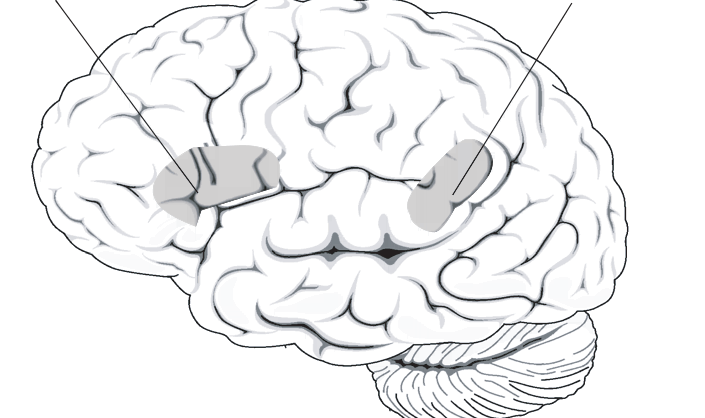
\includegraphics[width=6.2cm]{language_areas.png}};
        \begin{scope}[x={(img.south east)}, y={(img.north west)}]
          \node[regionlabel, fill=mint!60!cardwhite, anchor=south west] at (0,0.99) {Բրոկայի շրջան};
          \node[regionlabel, fill=lavender!70!cardwhite, anchor=south, visible on=<2->] at (0.81,0.99) {Վերնիկեի շրջան};
          \node[font=\scriptsize, text=plum!70!cream, anchor=north west] at (0.0,0.02) {ձախ կիսագունդ, ճակատը՝ ձախում};
        \end{scope}
      \end{tikzpicture}
    \end{column}
    \begin{column}{0.46\textwidth}
      \begin{card}[colback=mint!35!cardwhite]
        {\blackfont Բրոկայի շրջան} (Broca's area)\par
        Ճակատային բլիթ։ Խոսքի \textbf{կառուցումը}. միտքը ձևակերպել, բառերը ճիշտ դասավորել
      \end{card}
      \onslide<2->{%
      \begin{card}[colback=lavender!40!cardwhite]
        {\blackfont Վերնիկեի շրջան} (Wernicke's area)\par
        Քունքային բլիթ։ Խոսքի \textbf{հասկացումը}. բառերի իմաստը
      \end{card}}
    \end{column}
  \end{columns}
  \vspace{1mm}
  \onslide<3->{{\small Գտել են 19-րդ դարում՝ ուսումնասիրելով մարդկանց, ովքեր վնասվածք էին ստացել \textbf{հենց ճիշտ տեղում}։ Գոնե վնասվածքները իրենք չէին հասցնում (որքան գիտենք)։}\par}
\end{frame}

% Broca's (expressive) aphasia
\begin{frame}{Բրոկայի աֆազիա}
  \begin{columns}[c]
    \begin{column}{0.58\textwidth}
      \begin{itemize}
        \item \textbf{Աֆազիա} (aphasia)՝ խոսքի կամ հասկացողության խանգարում ուղեղի վնասվածքից
        \item Բրոկայի (էքսպրեսիվ) աֆազիա. մարդը \textbf{հասկանում է}, բերանն ու լեզուն առողջ են, բայց սահուն խոսել չի կարողանում
        \item<2-> Հաճախ խանգարված է նաև \textbf{գիրը}։ Բերանն ու ձեռքը տարբեր են, ուրեմն խնդիրը ընդհանուր մասում է՝ \textbf{լեզվի մշակման}
      \end{itemize}
    \end{column}
    \begin{column}{0.38\textwidth}
      \centering
      \begin{tikzpicture}
        \node (m) at (0,0) {\mascot[2.5cm]{thinking}};
        \node[say, callout absolute pointer={(m.north)}, font=\handfont\large] at (0.3,2.2) {Ես... խանութ... հաց...};
      \end{tikzpicture}
    \end{column}
  \end{columns}
\end{frame}

% Wernicke's aphasia: fluent nonsense
\begin{frame}{Վերնիկեի աֆազիա}
  \begin{columns}[c]
    \begin{column}{0.5\textwidth}
      \begin{itemize}
        \item Մարդը \textbf{չի հասկանում} բառերը, թեև զգում է տոնն ու ռիթմը
        \item Խոսում է սահուն ու երկար, բայց իրական ու հորինված բառերի խառնուրդով
        \item<3-> Ու ինքը դա \textbf{չի նկատում}։ Պատկերացրու հիասթափությունը
      \end{itemize}
    \end{column}
    \begin{column}{0.46\textwidth}
      \begin{card}[colback=mint!35!cardwhite]
        {\blackfont\small Ուզում էր ասել}\par
        {\large Գնացի խանութ, հաց գնեցի։}
      \end{card}
      \vspace{2mm}
      \onslide<2->{%
      \begin{card}[colback=lavender!40!cardwhite]
        {\blackfont\small Ասաց}\par
        {\handfont\large Ես գնացիլ խանութ-փանութ այսօրօրօր, գնեցիկ-թնեցիկ հաց-կաց-թաց...}
      \end{card}}
    \end{column}
  \end{columns}
\end{frame}

% Brain scans widened the map
\begin{frame}{Սկաներներից հետո քարտեզը մեծացավ}
  \begin{columns}[c]
    \begin{column}{0.5\textwidth}
      \centering
      \begin{tikzpicture}
        \node[anchor=south west, inner sep=0] (img) at (0,0) {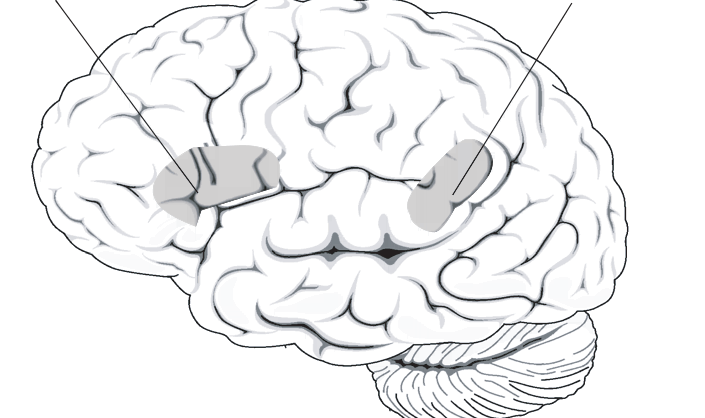
\includegraphics[width=6cm]{language_areas.png}};
        \begin{scope}[x={(img.south east)}, y={(img.north west)}]
          \begin{scope}[visible on=<2->]
            \fill[lavender, opacity=0.75, rotate around={-6:(0.5,0.44)}] (0.5,0.44) ellipse [x radius=1.35cm, y radius=0.18cm];
            \fill[peach, opacity=0.75, rotate around={-8:(0.5,0.32)}] (0.5,0.32) ellipse [x radius=1.35cm, y radius=0.18cm];
            \node[regionlabel, fill=lavender!70!cardwhite] at (0.27,-0.09) {վերին քունքային};
            \node[regionlabel, fill=peach!70!cardwhite] at (0.73,-0.09) {միջին քունքային};
            \node[regionlabel, fill=butter!80!cardwhite] at (0.5,-0.23) {պուտամեն՝ խորքում};
          \end{scope}
          \node[regionlabel, fill=mint!60!cardwhite, anchor=south west] at (0,0.99) {Բրոկա};
          \node[regionlabel, fill=cardwhite, anchor=south] at (0.81,0.99) {Վերնիկե};
        \end{scope}
      \end{tikzpicture}
    \end{column}
    \begin{column}{0.46\textwidth}
      \begin{itemize}
        \item Բրոկան դեռ կարևոր է \textbf{շարահյուսության} (syntax) համար
        \item<2-> Վերնիկեն «պաշտոնազրկվել» է. խոսքը մշակում են քունքային բլթի \textbf{լայն} հատվածներ՝ լսողական կեղևի կողքին (գոնե մի անգամ տրամաբանական է)
        \item<3-> Լեզուն ցրված է ողջ ուղեղով, ուրեմն այն ուղեղի \textbf{հիմնարար} ֆունկցիա է
      \end{itemize}
    \end{column}
  \end{columns}
\end{frame}

% Linguistic relativity and the Sapir-Whorf joke
\begin{frame}{Լեզուն փոխո՞ւմ է մտածողությունը}
  \begin{columns}[T]
    \begin{column}{0.56\textwidth}
      \begin{itemize}
        \item \textbf{Լեզվական հարաբերականություն} (linguistic relativity). լեզուդ որոշում է, թե ինչպես ես մտածում
      \end{itemize}
      \onslide<2->{%
      \begin{bookquote}
        Եթե լեզվում «հուսալի» բառ չլիներ, մարդիկ չէին հասկանա հուսալիությունը ու կաշխատեին \textbf{անշարժ գույքի գործակալ}։
      \end{bookquote}}
      \onslide<3->{{\small Գույների քիչ անուններ ունեցող լեզուների հետազոտությունները \textbf{վիճելի} են։}\par}
    \end{column}
    \begin{column}{0.4\textwidth}
      \onslide<4->{%
      \begin{card}[colback=lavender!40!cardwhite]
        {\blackfont Սեփիր-Ուորֆի վարկած}\par\smallskip
        Սեփիրն ու Ուորֆը միասին ոչինչ չեն գրել ու վարկած չեն առաջարկել։ Վարկածը ծնվեց, երբ հորինեցին նրա \textbf{անունը}. հիանալի օրինակ հենց իր համար։
      \end{card}
      \centering\mascot[1.3cm]{confused}}
    \end{column}
  \end{columns}
\end{frame}

% Neurolinguistic programming
\begin{frame}{Նեյրոլեզվաբանական ծրագրավորում (NLP)}
  \begin{columns}[T]
    \begin{column}{0.5\textwidth}
      \begin{itemize}
        \item Հոգեթերապիայի ու «անձնական աճի» խառնուրդ
        \item Գաղափարը. փոխիր մարդու բառերը, ու կփոխվեն նրա մտածողությունն ու վարքը, ինչպես կոդից «բագ» ջնջելիս \emoji{computer}
        \item<2-> Ապացույցներ գրեթե չկան. \textbf{կեղծ գիտություն} է
      \end{itemize}
    \end{column}
    \begin{column}{0.46\textwidth}
      \onslide<2->{%
      \begin{bookquote}
        Ուղեղն անում է իր ուզածը, ինչ էլ որ աշխարհը շպրտի նրա վրա։ Դժվար թե «շարք կանգնի» մի խնամքով ընտրված արտահայտության առաջ։
      \end{bookquote}}
      \onslide<3->{%
      \begin{card}[colback=mint!35!cardwhite]
        Բայց մի բանում NLP-ն ճիշտ է. \textbf{ոչ բառային} շփումը շատ կարևոր է։
      \end{card}}
    \end{column}
  \end{columns}
\end{frame}

% Oliver Sacks: aphasia patients laughing at the president
\begin{frame}{Նախագահի ելույթը}
  \begin{columns}[c]
    \begin{column}{0.56\textwidth}
      \begin{itemize}
        \item Օլիվեր Սաքս, «Մարդը, ով կնոջը գլխարկի տեղ դրեց» (1985)
        \item Աֆազիայով պացիենտները դիտում են նախագահի ելույթը ու \textbf{քրքջում են}
        \item<2-> Բառերը չհասկանալով՝ նրանք նկատում են այն, ինչ մենք բաց ենք թողնում. դեմքի ջղաձգումներ, ժեստեր, ռիթմ։ \textbf{Ստի նշաններ}
      \end{itemize}
    \end{column}
    \begin{column}{0.38\textwidth}
      \centering
      \bigemoji[1.2cm]{tv}\ \bigemoji[1.2cm]{laughing}\par\medskip
      \onslide<3->{%
      \begin{bookquote}
        Երբ դա գալիս է աշխարհի ամենահզոր մարդուց, մնում է կամ ծիծաղել, կամ լացել։
      \end{bookquote}}
    \end{column}
  \end{columns}
\end{frame}

% Same words, different faces
\begin{frame}{Նույն բառերը, տարբեր դեմքեր}
  \centering
  \begin{tikzpicture}
    \foreach \i/\e/\t/\m/\s in {0/grin/{ուրախ}/{«Շնորհակալ եմ»}/1, 1/rage/{զայրացած}/{«Ինչ ես արել»}/2, 2/nauseated/{զզված}/{«Էս ի՞նչ է»}/3}{
      \begin{scope}[visible on=<\s->]
        \node (f\i) at (\i*4.6,0) {\bigemoji[1.3cm]{\e}};
        \node[say, callout absolute pointer={(f\i.north)}, font=\handfont\large] at (\i*4.6,1.35) {Պետք չէր...};
        \node[font=\blackfont\small, text=plum] at (\i*4.6,-1.0) {\t};
        \node[font=\small, text=plum!75!cream] at (\i*4.6,-1.4) {\m};
      \end{scope}}
  \end{tikzpicture}\par\vspace{1mm}
  \raggedright
  \onslide<4->{%
  \begin{tryit}
    Ասա «պետք չէր» երեք տարբեր դեմքով։ Բառերը նույնն են, իմաստը՝ բոլորովին տարբեր։
  \end{tryit}}
\end{frame}

% Universal expressions, and what we know today
\begin{frame}{Դեմքերը նույնն են ամենուր... թե՞ ոչ}
  \begin{columns}[T]
    \begin{column}{0.5\textwidth}
      \begin{itemize}
        \item Դեմքի արտահայտությունների նկարները ցույց են տվել տարբեր մշակույթների, նաև շատ հեռավոր ժողովուրդների
        \item Գրեթե բոլորը \textbf{ճանաչել են} դրանք
        \item Բըրնեթի եզրակացությունը. դիմախաղը \textbf{բնածին} է։ Ամազոնում ու Նյու Յորքում զարմանում են նույն դեմքով
      \end{itemize}
    \end{column}
    \begin{column}{0.46\textwidth}
      \onslide<2->{%
      \begin{scienceupdate}
        Այսօր սա \textbf{վիճելի} է։ Հին փորձերում ընտրում էին պատրաստի բառերից։ Երբ Նամիբիայի հիմբա ժողովրդին խնդրեցին նկարներն \textbf{ազատ} դասավորել, «համընդհանուր» վեց խումբը չստացվեց։ Դեմքով զգացմունք արտահայտելը շատ է տարբերվում մշակույթից ու իրավիճակից։
      \end{scienceupdate}}
    \end{column}
  \end{columns}
  \source{Gendron et al., Emotion, 2014; Barrett et al., Psychol. Sci. Public Interest, 2019}
\end{frame}

% Emoticons: lines and dots are enough
\begin{frame}{Երկու կետ ու փակագիծ}
  \centering
  \begin{tikzpicture}
    \foreach \i/\s/\t in {0/{:-)}/ուրախություն, 1/{:-(}/տխրություն, 2/{>:-(}/զայրույթ, 3/{:-O}/զարմանք}{
      \node[draw=plum, line width=0.8pt, fill=cardwhite, rounded corners=3mm, minimum width=2.6cm, minimum height=1.4cm,
            font=\blackfont\fontsize{26}{28}\selectfont, text=plum] (e\i) at (\i*3.3,0) {\s};
      \node[font=\small, text=plum, below=1mm of e\i, visible on=<2->] {\t};}
  \end{tikzpicture}\par\vspace{3mm}
  \raggedright
  \begin{columns}[c]
    \begin{column}{0.54\textwidth}
      Պարզ գծեր ու կետեր են, \textbf{նույնիսկ ուղղահայաց չեն}, բայց ուղեղը միանգամից դեմք է տեսնում։ Տեսողական կեղևն ունի դեմքերի համար առանձին հատվածներ (5-րդ գլուխ)։
    \end{column}
    \begin{column}{0.42\textwidth}
      \onslide<3->{%
      \begin{chatbox}
        Գրիր որևէ զգացմունք \textbf{միայն կետադրական նշաններով}։ Մյուսները թող գուշակեն։
      \end{chatbox}}
    \end{column}
  \end{columns}
\end{frame}

% Why faces matter: alarm and feedback
\begin{frame}{Դեմքը՝ ահազանգ ու ուղեցույց}
  \begin{columns}[c]
    \begin{column}{0.54\textwidth}
      \begin{tikzpicture}
        \node[say, text width=6cm, align=left, font=\handfont\normalsize] (s) at (0,0)
          {Չեմ ուզում քեզ անհանգստացնել, բայց կատաղած բորենիների ոհմակ է գալիս մեր վրա...};
        \node[anchor=north, text width=6.4cm, font=\small, text=plum, visible on=<2->] at ([yshift=-3mm]s.south)
          {...մինչև նախադասության վերջը նրանք կհասնեին։ Վախեցած դեմքն \textbf{ավելի արագ} է։};
      \end{tikzpicture}
      \begin{itemize}
        \item<3-> Բոլորը վախեցած են. ուղեղը պատրաստվում է փախչել
        \item<3-> Բոլորը ցնցված են ու զզված. \textbf{անմիջապես կանգնիր}
      \end{itemize}
    \end{column}
    \begin{column}{0.42\textwidth}
      \onslide<4->{%
      \begin{card}[colback=mint!35!cardwhite]
        \emoji{eyes}\ Դեմքեր կարդալիս ակտիվ է \textbf{նշաձև մարմինը} (amygdala)։ Այն մշակում է մեր զգացմունքները ու, երևում է, պետք է նաև ուրիշներինը ճանաչելու համար։ Զզվանքի համար՝ նաև \textbf{պուտամենը}։
      \end{card}}
    \end{column}
  \end{columns}
\end{frame}

% Poker face, until the meteorite
\begin{frame}{Պոկերի դեմք}
  \begin{columns}[c]
    \begin{column}{0.54\textwidth}
      \begin{itemize}
        \item Պոկերիստները պահում են չեզոք (կամ սուտ) դեմք, որ չմատնեն իրենց խաղաքարտերը
        \item 52 խաղաքարտով տարբերակները սահմանափակ են. կարելի է պատրաստվել բոլորին, նույնիսկ անպարտելի «սթրեյթ ֆլեշին»
        \item Երբ գիտես՝ ինչ կարող է լինել, \textbf{գիտակցված} կառավարումը հաղթում է
      \end{itemize}
    \end{column}
    \begin{column}{0.4\textwidth}
      \centering
      \bigemoji[1.2cm]{joker}\par\medskip
      \onslide<2->{%
      \begin{card}[colback=peach!35!cardwhite]
        Բայց եթե խաղի ժամանակ երկնաքարը ծակի առաստաղն ու ընկնի սեղանին, դժվար թե որևէ մեկը կարողանա \textbf{չզարմանալ} \emoji{exploding}
      \end{card}}
    \end{column}
  \end{columns}
\end{frame}

% Voluntary vs involuntary expressions, and the meme
\begin{frame}{Ժպտալ՝ ատամները սեղմած}
  \begin{columns}[c]
    \begin{column}{0.52\textwidth}
      \begin{card}[colback=mint!35!cardwhite]
        {\blackfont Կամային} դիմախաղ. \textbf{շարժիչ կեղև} (motor cortex)։ Ոգևորված դեմք ընկերոջդ ձանձրալի լուսանկարներին նայելիս
      \end{card}
      \begin{card}[colback=peach!35!cardwhite]
        {\blackfont Ակամա} դիմախաղ. \textbf{լիմբիկ համակարգ}, իրական զգացմունքներ
      \end{card}
      \onslide<2->{{\small Նոր կեղևը կարող է ստել, իսկ լիմբիկ համակարգը \textbf{միշտ ազնիվ է}։ Ու նրանք հաճախ են բախվում։}\par}
    \end{column}
    \begin{column}{0.44\textwidth}
      \centering
      \onslide<3->{%
      \begin{meme}[5.4cm]{they_dont_know.png}
        \memecap[text width=2.5cm, font=\blackfont\footnotesize]{0.76}{0.88}{Նրանք չգիտեն, որ ժպիտս կեղծ է}
      \end{meme}}
    \end{column}
  \end{columns}
\end{frame}

% ===== Section 2: "Carrots and sticks" (compliance techniques and why they work) (~18 min) + break =====
\partaccent{butter}
\topicopener{carrot}{Համոզելու հնարքներ}{Գազար ու փայտ}{Ինչպես ենք կառավարում ուրիշներին, ու ինչպես են կառավարում մեզ}{smug}

% Burnett buys a car (and takes his dad)
\begin{frame}{Բըրնեթը մեքենա է գնում}
  \begin{columns}[c]
    \begin{column}{0.55\textwidth}
      \begin{itemize}
        \item Այնքան մեքենա ես տեսնում, որ սկսում ես մտածել՝ բակում ձիու համար տեղ կլինի՞
        \item Անիվներին քացի ես տալիս, որ գիտակ երևաս։ \textbf{Կոշիկիդ ծայրը կարո՞ղ է ռետին վերլուծել}
        \item<2-> Իսկ ամենավատը վաճառողներն են. կեղծ ընկերականություն, «պետք է մենեջերին հարցնեմ»
      \end{itemize}
    \end{column}
    \begin{column}{0.41\textwidth}
      \centering
      \bigemoji[1.1cm]{car}\ \bigemoji[1.1cm]{moneybag}\par\medskip
      \onslide<3->{%
      \begin{card}[colback=butter!45!cream]
        Դրա համար Բըրնեթը միշտ \textbf{հորն} է տանում։ Հոր մարտավարությունը. հայհոյել վաճառողներին ու հանցագործ անվանել, մինչև գինն իջեցնեն։\par\smallskip
        Ոչ նրբանկատ, բայց \textbf{արդյունավետ} \emoji{angry}
      \end{card}}
    \end{column}
  \end{columns}
\end{frame}

% Why do sales tricks work at all?
\begin{frame}{Ինչու են հնարքներն աշխատում}
  \begin{columns}[c]
    \begin{column}{0.58\textwidth}
      \begin{itemize}
        \item Գնորդները բոլորովին տարբեր են, բայց նույն հնարքները աշխատում են \textbf{ամենուր}
        \item Կան վարքեր, որոնք մեծացնում են \textbf{զիջողականությունը} (compliance). մարդը համաձայնում է դիմացինի խնդրանքին
        \item<3-> Բայց մարդուն ամբողջությամբ կառավարել չի կարելի, ինչ էլ որ պնդեն «գայթակղության գուրուները»
      \end{itemize}
    \end{column}
    \begin{column}{0.38\textwidth}
      \centering
      \onslide<2->{%
      \begin{card}[colback=butter!45!cream]
        \centering
        \bigemoji[0.9cm]{flushed}\ \bigemoji[0.9cm]{crown}\ \bigemoji[0.9cm]{heart}\par\smallskip
        Կարող ես բարկանալ աթոռի վրա, բայց ամոթը, հպարտությունն ու սերը առանց ուրիշների \textbf{չկան}
      \end{card}}
    \end{column}
  \end{columns}
\end{frame}

% Foot in the door: the escalating friend
\begin{frame}{Ոտքը դռան արանքում (foot-in-the-door)}
  \centering
  \begin{tikzpicture}
    \foreach \i/\e/\t/\s in {0/dollar/{Ավտոբուսի\\ փող}/1, 1/bread/{Մի սենդվիչ\\ էլ}/2,
                             2/beer/{Բար. դու ես\\ վճարում, չէ՞}/3, 3/clinking/{Էլի մի քանի\\ բաժակ}/4,
                             4/taxi/{Տաքսի\\ տուն}/5}{
      \node[stairstep, fill=butter!45!cardwhite, text width=2.2cm, minimum height=1cm, anchor=south west,
            visible on=<\s->] (s\i) at (\i*2.6, \i*0.48) {\emoji{\e}\\ \t};}
    \draw[-{Stealth[length=3mm]}, plum, line width=1.4pt, visible on=<5->] (0,-0.3) -- (12.8,-0.3)
      node[midway, below, font=\small, text=plum] {ամեն քայլը նախորդից մի քիչ մեծ է};
  \end{tikzpicture}\par\vspace{1mm}
  \raggedright
  \onslide<6->{%
  \begin{card}[colback=butter!45!cream]
    Եթե միանգամից ասեր «կերակրիր, խմեցրու ու տաքսիով տուն ուղարկիր», կմերժեիր։ Բայց հենց \textbf{դա էլ արեցիր}։
  \end{card}}
\end{frame}

% Meme: Anakin and Padme
\begin{frame}{Ընդամենը ավտոբուսի փող}
  \centering
  \begin{meme}[6.3cm]{anakin_padme.jpg}
    \memecap[text width=2.6cm]{0.25}{0.6}{Ավտոբուսի փող կտա՞ս}
    \memecap[text width=2.4cm]{0.75}{0.6}{Ու վերջ, չէ՞}
    \memecap[text width=2.4cm]{0.75}{0.1}{Ու վերջ, չէ՞}
  \end{meme}
\end{frame}

% FITD limits
\begin{frame}{Ոտքը դռան արանքում. սահմանները}
  \begin{columns}[T]
    \begin{column}{0.31\textwidth}
      \begin{card}[colback=butter!45!cream]
        \centering\bigemoji[0.8cm]{hourglass}\par\smallskip
        \raggedright{\blackfont Ժամանակ է պետք}\par
        5000 դրամ պարտք տալուց 10 վայրկյան հետո 50\,000 չեն խնդրում
      \end{card}
    \end{column}
    \begin{column}{0.31\textwidth}
      \onslide<2->{%
      \begin{card}[colback=mint!35!cardwhite]
        \centering\bigemoji[0.8cm]{dove}\par\smallskip
        \raggedright{\blackfont Լավ գործ}\par
        Հսկել ես, մինչ ընկերդ նախկինի մեքենային հայհոյանք էր գրում։ Աղյուս նետելու նրան \textbf{չես տանի}
      \end{card}}
    \end{column}
    \begin{column}{0.31\textwidth}
      \onslide<3->{%
      \begin{card}[colback=lavender!40!cardwhite]
        \centering\bigemoji[0.8cm]{snake}\par\smallskip
        \raggedright{\blackfont Նույն տեսակը}\par
        Տուն հասցնելը չի նշանակում, որ մի ամիս կպահես նրա \textbf{պիթոնին}
      \end{card}}
    \end{column}
  \end{columns}
  \vspace{3mm}
  \onslide<4->{\centering «Խորքում մարդիկ հաճախ բավական բարի են»։ Բըրնեթ\par}
\end{frame}

% Family tech support; FITD by email
\begin{frame}{Ընտանիքի 24/7 տեխսպասարկումը}
  \begin{columns}[c]
    \begin{column}{0.47\textwidth}
      \begin{poll}
        \emoji{computer}\,\emoji{phone}\par\smallskip
        Բարձրացրու ձեռքդ, եթե մի անգամ կարգավորեցիր ծնողներիդ հեռախոսն ու դարձար նրանց \textbf{24/7 տեխնիկական աջակցությունը}։
      \end{poll}
      \vspace{2mm}
      \onslide<2->{\small Սա էլ է ոտքը դռան արանքում։\par}
    \end{column}
    \begin{column}{0.47\textwidth}
      \onslide<3->{%
      \begin{card}
        \emoji{memo}\ {\blackfont Գեգեն (Guéguen), 2002}\par\smallskip
        Էլ. նամակով խնդրել են բացել ֆայլ։ Համաձայնողներն ավելի հաճախ էին մասնակցում հետո խնդրված \textbf{ավելի ծանր} հարցմանը։ Դեմք ու ձայն պետք չեն։
      \end{card}}
      \onslide<4->{%
      \begin{bookquote}
        Ուղեղը մտահոգիչ պատրաստակամությամբ է համաձայնում խնդրանքներին։
      \end{bookquote}}
    \end{column}
  \end{columns}
\end{frame}

% Door in the face
\begin{frame}{Դուռը երեսին (door-in-the-face)}
  \begin{columns}[c]
    \begin{column}{0.5\textwidth}
      \begin{tikzpicture}
        \node[chatmsg=5.6cm, fill=butter!45!cardwhite, anchor=north west] (r1) at (0,0)
          {Կարո՞ղ եմ իմ \textbf{բոլոր իրերը} պահել քո տանը, մինչ տեղափոխվում եմ};
        \node[chatmsg=1.6cm, fill=cardwhite, anchor=north east] (a1) at ([yshift=-2mm]r1.south east) {Ո՛չ \emoji{cross}};
        \node[chatmsg=5.6cm, fill=butter!45!cardwhite, anchor=north west, visible on=<2->] (r2)
          at ([yshift=-2mm]r1.south west |- a1.south) {Լավ, գոնե \textbf{մեքենադ} կտա՞ս հանգստյան օրերին՝ իրերս տեղափոխելու};
        \node[chatmsg=1.6cm, fill=cardwhite, anchor=north east, visible on=<2->] at ([yshift=-2mm]r2.south east) {Դե... լավ \emoji{check}};
      \end{tikzpicture}
    \end{column}
    \begin{column}{0.46\textwidth}
      \onslide<3->{%
      \begin{card}[colback=brainpink!25!cardwhite]
        Բայց մեքենադ ամբողջ հանգստյան օրերին ուրիշին տալն էլ է անհարմար։ Սովորաբար \textbf{երբեք չէիր համաձայնի}։
      \end{card}}
      \onslide<4->{%
      \begin{card}[colback=butter!45!cream]
        Դուռը երեսին փակողը \textbf{դու} ես։ Դա քեզ վատ է զգացնել տալիս, ու ուզում ես \textbf{փոխհատուցել}։
      \end{card}}
    \end{column}
  \end{columns}
\end{frame}

% Which is stronger? (book's numbers) + the Alpine cheese hut
\begin{frame}{Ո՞րն է ավելի ուժեղ}
  \begin{columns}[c]
    \begin{column}{0.4\textwidth}
      \centering
      \begin{tikzpicture}
        \begin{axis}[
            ybar, width=5.4cm, height=4cm, bar width=1.1cm,
            ymin=0, ymax=105, enlarge x limits=0.5,
            symbolic x coords={fitd, ditf},
            xtick={fitd, ditf}, % not xtick=data: two \addplot
            xticklabels={{Ոտքը դռան\\ արանքում}, {Դուռը\\ երեսին}},
            xticklabel style={align=center, font=\small, text=plum},
            axis line style={plum}, axis x line*=bottom, axis y line=none,
            nodes near coords={\pgfmathprintnumber{\pgfplotspointmeta}\%},
            nodes near coords style={font=\blackfont\small, text=plum},
            clip=false,
          ]
          \addplot[fill=amBlue, draw=none] coordinates {(fitd,60)};
          \addplot[fill=amRed, draw=none] coordinates {(ditf,90)};
        \end{axis}
      \end{tikzpicture}\par
      {\scriptsize Չան ու Աու, 2011. թվաբանական առաջադրանքն արած 6-8 տարեկաններ (գրքի թվերով)}
    \end{column}
    \begin{column}{0.56\textwidth}
      \onslide<2->{%
      \begin{bookquote}
        Ուզում ես, որ դպրոցականներն ինչ-որ բան անեն՝ դուռը փակիր նրանց երեսին։ (Հրապարակավ ավելի լավ է այլ կերպ ասել)
      \end{bookquote}}
      \onslide<3->{{\small \emoji{cheese}\ Աշխատում է նաև Ալպյան տնակից պանիր վաճառելիս (փորձերի մեծ մասը այնտեղ չի անցկացվում)}\par}
    \end{column}
  \end{columns}
  \source{Chan \& Au, Teaching and Teacher Education, 2011 (երեխաների տարիքը)}
\end{frame}

% Low-ball
\begin{frame}{Ցածր գնդակ (low-ball)}
  \begin{columns}[c]
    \begin{column}{0.54\textwidth}
      \begin{itemize}
        \item Համաձայնել ես գնին կամ ժամկետին, ու դիմացինը \textbf{հանկարծ բարձրացնում է} պահանջը
        \item Ջղայնանում ես, բայց մեծ մասամբ \textbf{համաձայնում ես}, թեև նա խախտեց պայմանավորվածությունը
        \item<2-> Եթե չափն անցնի՝ ոչ. 35\,000 դրամանոց օգտագործված DVD նվագարկիչը չես առնի քո ողջ խնայողություններով \textbf{ու առաջնեկով}
      \end{itemize}
    \end{column}
    \begin{column}{0.42\textwidth}
      \onslide<3->{%
      \begin{card}[colback=butter!45!cream]
        \emoji{coffee}\ {\blackfont Բըրգեր ու Կոռնելիուս, 2003}\par\smallskip
        Հարցաթերթիկ լրացնելու դիմաց խոստացել են \textbf{սուրճի բաժակ}, հետո ասել են, որ բաժակներ չկան։ Մեծ մասը միևնույն է լրացրել է։\par\smallskip
        Այսինքն՝ կարելի է մարդկանց \textbf{անվճար} աշխատեցնել։ Մոտավորապես։
      \end{card}}
    \end{column}
  \end{columns}
\end{frame}

% Cialdini 1978: the 7 a.m. experiment
\begin{frame}{Ժամը 7-ին՝ համալսարանում}
  \begin{columns}[c]
    \begin{column}{0.52\textwidth}
      \centering
      \begin{tikzpicture}
        \begin{axis}[
            ybar, width=7cm, height=5cm, bar width=0.8cm,
            ymin=0, ymax=112, enlarge x limits=0.42,
            symbolic x coords={agree, came},
            xtick={agree, came},
            xticklabels={{համաձայնեցին}, {եկան\\ (համաձայնածներից)}},
            xticklabel style={align=center, font=\small, text=plum},
            axis line style={plum}, axis x line*=bottom, axis y line=none,
            nodes near coords={\pgfmathprintnumber{\pgfplotspointmeta}\%},
            nodes near coords style={font=\blackfont\small, text=plum},
            legend style={at={(0.5,1.02)}, anchor=south, draw=none, fill=none, font=\scriptsize, text=plum,
              legend columns=1, cells={anchor=west}},
            clip=false,
          ]
          \addplot[fill=amBlue, draw=none] coordinates {(agree,31) (came,79)};
          \addplot[fill=amOrange, draw=none] coordinates {(agree,56) (came,95)};
          \legend{{միանգամից ասել են՝ ժամը 7-ին}, {նախ «կմասնակցե՞ս», հետո՝ ժամը}}
        \end{axis}
      \end{tikzpicture}
    \end{column}
    \begin{column}{0.44\textwidth}
      \begin{itemize}
        \item Չալդինի և գործընկերներ, 1978. ուսանողներին հրավիրել են հոգեբանական փորձի
        \item Մի խմբին միանգամից ասել են, որ այն \textbf{առավոտյան 7-ին} է, մյուսին՝ միայն համաձայնելուց հետո
        \item<2-> Գլխավորը \textbf{կամավոր} համաձայնությունն է. դրանից հետո կառչում ենք որոշումից
      \end{itemize}
    \end{column}
  \end{columns}
  \source{Cialdini et al., J. Pers. Soc. Psychol., 1978}
\end{frame}

% Why: impression management
\begin{frame}{Տպավորության կառավարում}
  \begin{columns}[c]
    \begin{column}{0.4\textwidth}
      \centering
      \begin{tikzpicture}
        \node (m) at (0,0) {\mascot[2.4cm]{smug}};
        \node[draw=plum, dashed, line width=0.7pt, fill=cardwhite, rounded corners=2mm, font=\handfont\normalsize,
              text=plum, align=center] at (-0.2,2.2) {(մտքում) Էս ինչ\\ տգեղ երեխա է...};
        \node[say, callout absolute pointer={(m.east)}, font=\handfont\normalsize, visible on=<2->] at (1.9,0.9) {Վա՜յ, ինչ\\ անուշն է};
      \end{tikzpicture}
    \end{column}
    \begin{column}{0.56\textwidth}
      \begin{itemize}
        \item 4-րդ գլխից գիտենք, որ ուղեղը ընդունակ է ինքնավերլուծության
        \item<2-> Լեզուդ կծում ես. ճշմարտությունը քեզ վատ ցույց կտար
        \item<3-> Սա \textbf{տպավորության կառավարում} է (impression management). կառավարում ենք, թե ինչ կմտածեն մեր մասին
        \item<4-> Ուրիշների կարծիքը մեզ հետաքրքրում է \textbf{նյարդաբանական} մակարդակում
      \end{itemize}
    \end{column}
  \end{columns}
\end{frame}

% Farrow et al.: the brain is always in "look good" mode
\begin{frame}{Ուղեղը միշտ «լավ երևալու» ռեժիմում է}
  \begin{columns}[c]
    \begin{column}{0.58\textwidth}
      \begin{itemize}
        \item Ֆարոու և գործընկերներ, 2014. սկաների մեջ մարդիկ ընտրում էին վարքեր, որ \textbf{լավ} կամ \textbf{վատ} երևան
        \item Լրացուցիչ շրջաններ ակտիվանում էին \textbf{միայն} վատ երևալ փորձելիս։ «Լավ երևալը» ավելի արագ էր ու սովորականից չէր տարբերվում
        \item<2-> Եզրակացություն. ուղեղը \textbf{անընդհատ} է մեզ լավ ցույց տալիս
        \item<3-> Ընդամենը 20 մասնակից էր, բայց տարբերությունը ցնցող է
      \end{itemize}
    \end{column}
    \begin{column}{0.38\textwidth}
      \centering
      \onslide<2->{%
      \begin{tikzpicture}
        \foreach \x in {0,...,4}{\foreach \y in {0,...,2}{\node at (\x*0.85+0.3*\y, \y*0.75) {\bigemoji[0.7cm]{tree}};}}
        \node at (3.3,2.3) {\bigemoji[0.9cm]{magnifier}};
      \end{tikzpicture}\par\smallskip
      {\small Սկաներով այն փնտրելը նույնն է, թե անտառում փնտրես \textbf{մի կոնկրետ ծառ}}}
    \end{column}
  \end{columns}
\end{frame}

% Three techniques, one reason: we want to be liked
\begin{frame}{Երեք հնարք, մեկ պատճառ}
  \begin{tikzpicture}[x=1cm, y=1cm]
    \foreach \i/\c/\n/\r/\s in {
        0/butter/{Ոտքը դռան արանքում}/{Համաձայնել ես։ Հաջորդ նման խնդրանքը մերժելը կհիասթափեցնի ու կփչացնի կարծիքը քո մասին}/1,
        1/brainpink/{Դուռը երեսին}/{Մերժել ես մեծը ու գիտես, որ դիմացինը քեզ դրա համար չի սիրի։ Փոքրին համաձայնում ես որպես «մխիթարանք»}/2,
        2/lavender/{Ցածր գնդակ}/{Արդեն համաձայնել ես։ Հետ կանգնելը կհիասթափեցնի ու քեզ վատ ցույց կտա}/3}{
      \node[personnode, fill=\c!55!cardwhite, text width=3.2cm, minimum height=1.15cm, font=\blackfont\small, visible on=<\s->]
        (t\i) at (0,-\i*1.38) {\n};
      \node[personnode, text width=8.6cm, minimum height=1.15cm, anchor=west, align=left, visible on=<\s->]
        (r\i) at (2.6,-\i*1.38) {\r};
      \draw[-{Stealth[length=2.5mm]}, plum, line width=1pt, visible on=<\s->] (t\i) -- (r\i);}
  \end{tikzpicture}\par\vspace{3mm}
  \onslide<4->{%
  \begin{card}[colback=butter!45!cream]
    Երեքն էլ օգտագործում են մեր ցանկությունը, որ մեր մասին \textbf{լավ մտածեն}։ Այն այնքան ուժեղ է, որ հաղթում է տրամաբանությանը։
  \end{card}}
\end{frame}

% Consistency, reciprocity, dominance
\begin{frame}{Եվս երեք պատճառ}
  \begin{columns}[T]
    \begin{column}{0.32\textwidth}
      \begin{card}[colback=butter!45!cream]
        \centering\bigemoji[0.8cm]{link}\par\smallskip
        \raggedright{\blackfont Հետևողականություն}\par
        Արդեն փող տվել ես, ուրեմն ուղեղը որոշում է, որ \textbf{ուզում ես} էլի տալ։ Այլապես դիսոնանս է
      \end{card}
    \end{column}
    \begin{column}{0.32\textwidth}
      \onslide<2->{%
      \begin{card}[colback=mint!35!cardwhite]
        \centering\bigemoji[0.8cm]{handshake}\par\smallskip
        \raggedright{\blackfont Փոխադարձություն}\par
        Փոքր խնդրանքը մեծից հետո ուղեղը ընկալում է որպես լավություն, որովհետև \textbf{ապուշ է}
      \end{card}}
    \end{column}
    \begin{column}{0.32\textwidth}
      \onslide<3->{%
      \begin{card}[colback=lavender!40!cardwhite]
        \centering\bigemoji[0.8cm]{crown}\par\smallskip
        \raggedright{\blackfont Գերիշխանություն}\par
        Հետ կանգնես՝ նշանակում է, որ նա քեզ կառավարեց։ Ո՛չ, կանես, որովհետև \textbf{բարի ես, անիծյալ}
      \end{card}}
    \end{column}
  \end{columns}
\end{frame}

% Summary of the section
\begin{frame}{Ուղեղը մեզ հեշտ թիրախ է դարձնում}
  \begin{columns}[c]
    \begin{column}{0.56\textwidth}
      Ուղեղը ստիպում է, որ ուզենք\par\smallskip
      \begin{enumerate}
        \item<1-> որ մեզ \textbf{սիրեն}
        \item<2-> լինել \textbf{վերևում}
        \item<3-> լինել \textbf{հետևողական}
      \end{enumerate}
      \vspace{2mm}
      \onslide<4->{Արդյունքում խոցելի ենք ամեն անսկզբունք մարդու առաջ, ով ուզում է մեր փողը ու մի քիչ սակարկել գիտի։\par}
    \end{column}
    \begin{column}{0.4\textwidth}
      \onslide<5->{%
      \begin{bookquote}
        Անհավանական բարդ օրգան է պետք, որպեսզի \textbf{այսքան հիմար} բան անի։
      \end{bookquote}
      \centering\mascot[2cm]{confused}}
    \end{column}
  \end{columns}
\end{frame}

% First half on one page
\begin{frame}{Առաջին կեսը՝ մեկ էջում}
  \begin{columns}[T]
    \begin{column}{0.31\textwidth}
      \begin{card}[colback=peach!35!cardwhite]\emoji{hug}\ {\blackfont Ուրիշ մարդիկ}\par Խմբեր կազմում են անգամ ապստամբները. շփումը պարտադիր է\end{card}
    \end{column}
    \begin{column}{0.31\textwidth}
      \begin{card}[colback=mint!35!cardwhite]\emoji{masks}\ {\blackfont Դեմքեր ու խոսք}\par Լեզուն ցրված է ողջ ուղեղով, իսկ դեմքը մատնում է այն, ինչ բառերը թաքցնում են\end{card}
    \end{column}
    \begin{column}{0.31\textwidth}
      \begin{card}[colback=butter!45!cream]\emoji{carrot}\ {\blackfont Համոզում}\par Երեք հնարքն էլ աշխատում են, որովհետև ուզում ենք, որ մեզ սիրեն\end{card}
    \end{column}
  \end{columns}
  \vspace{2mm}
  \centering
  \mascot[1.2cm]{happy}\par
  {\small Հարցեր կա՞ն մինչև ընդմիջումը}
\end{frame}

% ---------------------------------------------------------------- break
\begin{frame}[plain]
  \begin{tikzpicture}[remember picture, overlay]
    \fill[butter!60!cream] (current page.south west) rectangle (current page.north east);
    \node at ([yshift=8mm]current page.center) {\mascot[4cm]{sleepy}};
    \node[anchor=north, font=\titlefont\fontsize{30}{32}\selectfont, text=plum] at ([yshift=-17mm]current page.center) {Ընդմիջում};
    \node[anchor=north, font=\mediumfont\large, text=plum] at ([yshift=-31mm]current page.center)
      {5 րոպե \emoji{coffee}\quad Կանգնիր, ձգվիր, ջուր խմիր};
  \end{tikzpicture}
\end{frame}

% ===== Section 3: "Achy Breaky Brain" (love, monogamy, break-ups) (~14 min) =====
\partaccent{brainpink}
\topicopener{brokenheart}{Սեր ու բաժանում}{Կոտրված սիրտ, ցավող ուղեղ}{Ինչու է բաժանումն այդքան ավերիչ}{sad}

% Heartbreak: nothing physical happened, so why does it hurt so much?
\begin{frame}{Բազմոցին, վարագույրները փակ}
  \begin{columns}[c]
    \begin{column}{0.44\textwidth}
      \begin{bookquote}
        Երբևէ օրերով պառկե՞լ ես բազմոցին կծկված, վարագույրները փակ, հեռախոսը չպատասխանած, ու մտածել, թե ինչու է ամբողջ տիեզերքը որոշել քեզ տանջել։
      \end{bookquote}
    \end{column}
    \begin{column}{0.52\textwidth}
      \begin{itemize}
        \item Ներշնչում է մեծ արվեստ ու երաժշտություն, ինչպես նաև \textbf{սարսափելի պոեզիա}
        \item<2-> Բայց ֆիզիկապես \textbf{ոչինչ չի պատահել}. ոչ վնասվածք, ոչ վիրուս
        \item<3-> Ինչու՞ է ամիսներով ցավում։ Որովհետև ուրիշները \textbf{մեծ ազդեցություն} ունեն ուղեղի բարօրության վրա
      \end{itemize}
    \end{column}
  \end{columns}
\end{frame}

% Culture is obsessed with couples; monogamy is odd for a primate
\begin{frame}{Ամբողջ մշակույթը զույգերի մասին է}
  \begin{columns}[c]
    \begin{column}{0.46\textwidth}
      \chip{heart}{Վալենտինի օր} \chip{couple}{հարսանիքներ}\par\smallskip
      \chip{film}{ռոմանտիկ կատակերգություններ}\par\smallskip
      \chip{musical}{սիրո բալլադներ} \chip{sparkles}{զարդեր}\par\smallskip
      \chip{memo}{պոեզիայի կեսը} \chip{loveletter}{բացիկներ}\par\medskip
      \onslide<3->{%
      \begin{chatbox}
        Գրիր բաժանման մասին ամենատխուր երգը, որ գիտես։
      \end{chatbox}}
    \end{column}
    \begin{column}{0.5\textwidth}
      \begin{itemize}
        \item Մոնոգամիան (մեկ զուգընկեր) մյուս պրիմատների մոտ \textbf{ընդունված չէ}
        \item<2-> Մենք ավելի երկար ենք ապրում ու կարող էինք շատ զուգընկերներ ունենալ։ Ավելի շատ զուգընկեր՝ ավելի շատ գեներ
        \item<2-> Բայց մարդիկ մեծ մասամբ ընտրում են \textbf{մեկին}
      \end{itemize}
    \end{column}
  \end{columns}
\end{frame}

% Why monogamy: three theories
\begin{frame}{Ինչու՞ մոնոգամիա. երեք վարկած}
  \begin{columns}[T]
    \begin{column}{0.31\textwidth}
      \begin{card}[colback=brainpink!25!cardwhite]
        \centering\bigemoji[0.8cm]{family}\par\smallskip
        \raggedright{\blackfont Երկու ծնող}\par
        Երկուսով խնամված երեխան ավելի հավանական է, որ գոյատևի
      \end{card}
    \end{column}
    \begin{column}{0.31\textwidth}
      \onslide<2->{%
      \begin{card}[colback=butter!45!cream]
        \centering\bigemoji[0.8cm]{moneybag}\par\smallskip
        \raggedright{\blackfont Մշակույթ}\par
        Հարստությունը պետք էր պահել ընտանիքում։ Իսկ ժառանգություն չես թողնի, եթե չգիտես՝ ով է քո ընտանիքը
      \end{card}}
    \end{column}
    \begin{column}{0.31\textwidth}
      \onslide<3->{%
      \begin{card}[colback=lavender!40!cardwhite]
        \centering\bigemoji[0.8cm]{baby}\par\smallskip
        \raggedright{\blackfont Տատիկներ}\par
        Տատիկներն օգնում էին թոռներին։ Բայց ոչ մի տատիկ չի խնամի երեխայի \textbf{նախկինի} երեխաներին
      \end{card}}
    \end{column}
  \end{columns}
  \vspace{3mm}
  \onslide<4->{\centering\small Ինչ էլ որ լինի պատճառը, սիրահարվելիս ուղեղը շատ տարօրինակ բաներ է անում։\par}
\end{frame}

% Attraction: antlers and tails
\begin{frame}{Գրավչություն. եղջյուրներ ու փետուրներ}
  \begin{columns}[c]
    \begin{column}{0.42\textwidth}
      \centering
      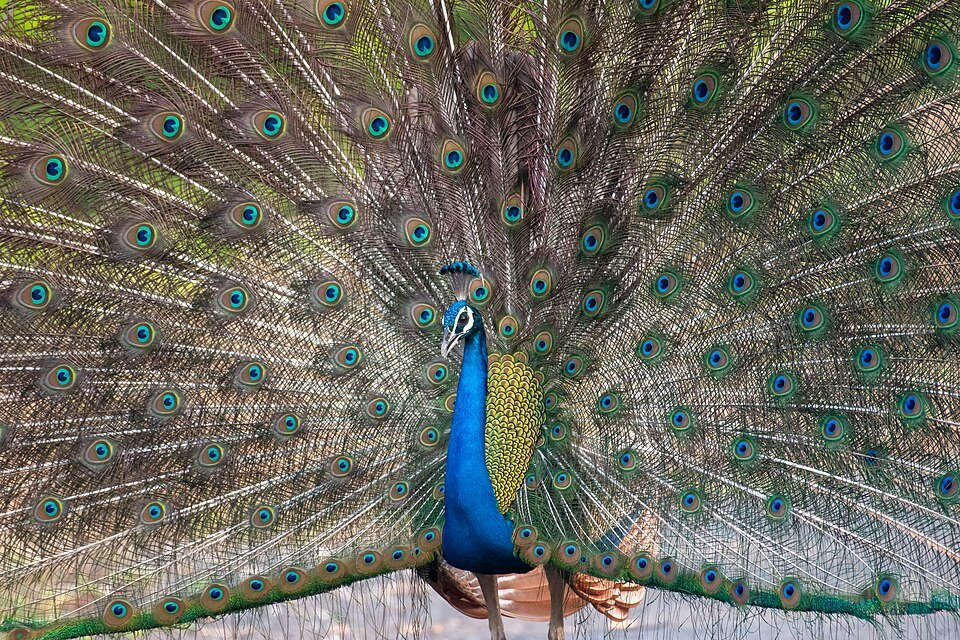
\includegraphics[width=\linewidth]{peacock.jpg}\par
      {\scriptsize Սիրամարգի պոչը գեղեցիկ է, բայց բազմանալու համար պետք չէ}
    \end{column}
    \begin{column}{0.54\textwidth}
      \begin{itemize}
        \item \textbf{Երկրորդային սեռական հատկանիշներ}. լոսի եղջյուրներ, սիրամարգի պոչ։ Ցույց են տալիս, թե որքան առողջ է կենդանին
        \item<2-> Մարդիկ էլ ունեն. խորը ձայն ու մորուք, կուրծք ու կորություններ
        \item<3-> Ինչն էր առաջինը՝ հատկանիշը, թե՞ ուղեղի սերը դրա նկատմամբ։ \textbf{Հավի ու ձվի} հարց
      \end{itemize}
    \end{column}
  \end{columns}
\end{frame}

% Preferences: wit, culture, and people who look like us
\begin{frame}{Ճաշակի հարց}
  \begin{columns}[T]
    \begin{column}{0.31\textwidth}
      \begin{card}[colback=mint!35!cardwhite]
        \centering\bigemoji[0.9cm]{bulb}\par\smallskip
        \raggedright{\blackfont Խելք}\par
        Ոմանց համար ամենագրավիչը մարդու սրամտությունն է
      \end{card}
    \end{column}
    \begin{column}{0.31\textwidth}
      \onslide<2->{%
      \begin{card}[colback=butter!45!cream]
        \centering\bigemoji[0.9cm]{earth}\par\smallskip
        \raggedright{\blackfont Մշակույթ}\par
        Արևմուտքում՝ արհեստական արևայրուք, Ասիայում՝ մաշկը \textbf{սպիտակեցնող} քսուքներ
      \end{card}}
    \end{column}
    \begin{column}{0.31\textwidth}
      \onslide<3->{%
      \begin{card}[colback=brainpink!25!cardwhite]
        \centering\bigemoji[0.9cm]{mirror}\par\smallskip
        \raggedright{\blackfont Նմանություն}\par
        Մեզ ավելի են գրավում \textbf{մեզ նման} մարդիկ։ Ուղեղի եսասիրությունը նորից
      \end{card}}
    \end{column}
  \end{columns}
\end{frame}

% Lust is not love: Bartels & Zeki
\begin{frame}{Ցանկություն $\neq$ սեր}
  \relax{\small Սեռական ցանկությունն (lust) ու սերը կոնկրետ մեկի հանդեպ ուղեղը մշակում է \textbf{տարբեր} կերպ։ Բարտելսն ու Զեկին սիրահարվածներին ցույց են տվել զուգընկերոջ նկարը.}\par\medskip
  \begin{columns}[T]
    \begin{column}{0.34\textwidth}
      \begin{card}[colback=mint!35!cardwhite]
        {\blackfont $\uparrow$ Ակտիվանում են}\par\smallskip
        կղզյակ (insula)\\
        գոտևոր կեղևի առաջային մաս\\
        պոչավոր կորիզ, պուտամեն
      \end{card}
    \end{column}
    \begin{column}{0.34\textwidth}
      \onslide<2->{%
      \begin{card}[colback=lavender!40!cardwhite]
        {\blackfont $\downarrow$ Հանգստանում են}\par\smallskip
        գոտևոր կեղևի հետին մաս՝ \textbf{ցավ}\\
        նշաձև մարմին՝ \textbf{վախ, զայրույթ}\\
        նախաճակատային կեղև՝ \textbf{տրամաբանություն}
      \end{card}}
    \end{column}
    \begin{column}{0.26\textwidth}
      \onslide<3->{%
      \centering\mascot[1.5cm]{smug}\par\smallskip
      \raggedright\small Դրա համար են զույգերն այդքան հանգիստ ու \textbf{ինքնագոհ} երևում}
    \end{column}
  \end{columns}
\end{frame}

% Dopamine: love works like a drug (meme)
\begin{frame}{Սերը՝ ինչպես թմրանյութ}
  \begin{columns}[c]
    \begin{column}{0.42\textwidth}
      \begin{itemize}
        \item Սիրահարվածությունը բարձրացնում է \textbf{դոֆամինի} ակտիվությունը պարգևի համակարգում
        \item Զուգընկերոջ ներկայությունը հաճույք է, \textbf{գրեթե թմրանյութի պես}
        \item Կախվածության մասին՝ 8-րդ գլխում
      \end{itemize}
    \end{column}
    \begin{column}{0.54\textwidth}
      \centering
      \onslide<2->{%
      \begin{meme}[7cm]{epic_handshake.jpg}
        \memecap{0.17}{0.4}{Սիրահարվածություն}
        \memecap{0.8}{0.55}{Թմրանյութեր}
        \memecap[font=\blackfont\large]{0.4}{0.9}{Դոֆամին}
      \end{meme}}
    \end{column}
  \end{columns}
\end{frame}

% Oxytocin and pheromones
\begin{frame}{Օքսիտոցին ու ֆերոմոններ}
  \begin{columns}[T]
    \begin{column}{0.5\textwidth}
      \begin{itemize}
        \item \textbf{Օքսիտոցին}՝ «սիրո հորմոն»։ Բըրնեթ. բարդ նյութի \textbf{ծիծաղելի պարզեցում} է։ Բարձր է զույգերի մոտ ու կապվում է վստահության հետ
      \end{itemize}
      \onslide<2->{%
      \begin{scienceupdate}
        Վստահության մասին պնդումը լավ չի կրկնվում. քթի սփրեյով օքսիտոցինի ազդեցությունը հետագա փորձերում չհաստատվեց։
      \end{scienceupdate}}
    \end{column}
    \begin{column}{0.46\textwidth}
      \onslide<3->{%
      \begin{card}[colback=brainpink!25!cardwhite]
        {\blackfont Ֆերոմոններ}\par\smallskip
«Ֆերոմոններով» սփրեյներ կան, բայց մարդկային «գրավչության» ֆերոմոնների \textbf{ապացույց չկա}։
      \end{card}}
      \onslide<4->{%
      \begin{bookquote}
        Ուղեղը հաճախ ապուշ է, բայց այդքան հեշտ էլ չի կառավարվում։
      \end{bookquote}}
    \end{column}
  \end{columns}
  \source{Nave, Camerer \& McCullough, Perspect. Psychol. Sci., 2015}
\end{frame}

% The partner becomes part of you
\begin{frame}{Զուգընկերը դառնում է քո մի մասը}
  \begin{columns}[c]
    \begin{column}{0.58\textwidth}
      \begin{itemize}
        \item Մի ամբողջ մարդ քեզ այդքան գնահատում է. մեծ \textbf{ձեռքբերում} է
        \item Զույգ լինելը սոցիալական կարգավիճակ է տալիս (ինչպես կասի ցանկացած երջանիկ միայնակ մարդ՝ \textbf{ատամները սեղմած})
        \item<2-> Ուղեղը հարմարվում է ու սկսում է այս ամենը \textbf{սպասել}. զուգընկերը մտնում է քո ծրագրերի ու նպատակների մեջ
      \end{itemize}
    \end{column}
    \begin{column}{0.38\textwidth}
      \centering
      \begin{tikzpicture}
        \fill[brainpink!35!cardwhite] (0,0) circle (1.2);
        \fill[lavender!55!cardwhite, visible on=<1>] (2.1,0) circle (1.2);
        \fill[lavender!55!cardwhite, visible on=<2->] (1.3,0) circle (1.2);
        \begin{scope}[visible on=<2->]
          \clip (0,0) circle (1.2);
          \fill[blush!70!cardwhite] (1.3,0) circle (1.2);
        \end{scope}
        \draw[plum, line width=0.9pt] (0,0) circle (1.2);
        \draw[plum, line width=0.9pt, visible on=<1>] (2.1,0) circle (1.2);
        \draw[plum, line width=0.9pt, visible on=<2->] (1.3,0) circle (1.2);
        \node[font=\blackfont, text=plum] at (-0.55,0) {Ես};
        \node[font=\blackfont, text=plum, visible on=<1>] at (2.6,0) {Նա};
        \node[font=\blackfont, text=plum, visible on=<2->] at (1.9,0) {Նա};
        \node[font=\blackfont\small, text=plum, visible on=<2->] at (0.65,0) {Մենք};
      \end{tikzpicture}
    \end{column}
  \end{columns}
\end{frame}

% And then it ends
\begin{frame}{Եվ հետո այն ավարտվում է}
  \begin{columns}[T]
    \begin{column}{0.46\textwidth}
      \begin{itemize}
        \item Անհավատարմություն, անհամատեղելիություն, մեկի վարքը վանեց մյուսին
        \item Տագնապային մարդիկ հակված են \textbf{ուռճացնել} կոնֆլիկտները, երբեմն՝ մինչև խզում
        \item<2-> Ինչքան բան էր ուղեղը ներդրել։ Ու այդ ամենը վերանում է \textbf{մեկ հարվածով}
      \end{itemize}
    \end{column}
    \begin{column}{0.5\textwidth}
      \onslide<3->{%
      \begin{card}[colback=brainpink!25!cardwhite]
        {\blackfont Ուղեղը միանգամից կորցնում է}\par\smallskip
        \emoji{gift}\ սպասվող բոլոր հաճելի զգացումները\par\smallskip
        \emoji{calendar}\ ապագայի ծրագրերը։ Իսկ ուղեղը \textbf{անորոշություն} չի սիրում\par\smallskip
        \emoji{house}\ գործնական պատասխանները. որտե՞ղ ապրեմ, ընկերներին կկորցնե՞մ
      \end{card}}
    \end{column}
  \end{columns}
\end{frame}

% Social pain, literally
\begin{frame}{Սա իսկապես ցավում է}
  \begin{columns}[T]
    \begin{column}{0.52\textwidth}
      \begin{itemize}
        \item Մեկը, ով քեզ ճանաչում է բոլորից լավ, որոշել է, որ \textbf{պետք չես}։ Հարված սոցիալական ինքնությանը
        \item<2-> Բաժանումը ակտիվացնում է այն շրջանները, որոնք մշակում են \textbf{ֆիզիկական ցավը}։ «Սերը ցավ է պատճառում»՝ բառացիորեն
        \item<2-> Պարացետամոլը երբեմն նույնիսկ օգնում է «սրտի ցավին»
      \end{itemize}
    \end{column}
    \begin{column}{0.44\textwidth}
      \onslide<3->{%
      \begin{scienceupdate}
        2014-ին նույն տվյալները վերլուծեցին ավելի նուրբ մեթոդով։ Շրջանները մասամբ համընկնում են, բայց ակտիվության \textbf{նախշերը տարբեր} են։ Նման է ցավին, բայց \textbf{նույնը չէ}։
      \end{scienceupdate}}
    \end{column}
  \end{columns}
  \source{Kross et al., PNAS, 2011; Woo et al., Nat. Commun., 2014}
\end{frame}

% Memories turn sour; withdrawal
\begin{frame}{Հիշողություններ ու «զրկանք»}
  \begin{columns}[c]
    \begin{column}{0.58\textwidth}
      \begin{itemize}
        \item Անհամար երջանիկ հիշողություններ հիմա կապված են \textbf{ցավի} հետ։ Սա խարխլում է քո «ես»-ի մի մեծ մասը
        \item<2-> Սովոր էիր մշտական պարգևի, ու այն հանկարծ վերցրին
        \item<3-> Մի բան, որ նման է թմրանյութից \textbf{զրկվելուն} (withdrawal)։ Ավելին՝ 8-րդ գլխում
      \end{itemize}
    \end{column}
    \begin{column}{0.38\textwidth}
      \centering
      \bigemoji[1cm]{camera}\ \bigemoji[1cm]{loveletter}\ \bigemoji[1cm]{musical}\par\medskip
      {\Large$\downarrow$}\par\medskip
      \bigemoji[1.4cm]{brokenheart}
    \end{column}
  \end{columns}
\end{frame}

% Recovery: it does get better
\begin{frame}{Ժամանակը իսկապես բուժում է}
  \begin{columns}[c]
    \begin{column}{0.58\textwidth}
      \begin{itemize}
        \item Ուղեղը կարողանում է ամեն ինչ \textbf{նորից հավաքել}, թեև դանդաղ
        \item<2-> Երբ կենտրոնանում ես բաժանման \textbf{դրական հետևանքների} վրա (օրինակ՝ գրելով), ավելի արագ ես վերականգնվում
        \item<3-> Գիտությունն ու կլիշեն համընկնում են. ժամանակի հետ \textbf{ավելի լավ է դառնում}
      \end{itemize}
      \onslide<4->{%
      \begin{bookquote}
        «Բաժանվելը դժվար է» ասելը շատ մեղմ է ասված։
      \end{bookquote}}
    \end{column}
    \begin{column}{0.38\textwidth}
      \centering
      \bigemoji[1.2cm]{sunrise}\par\medskip
      \mascot[2.3cm]{happy}
    \end{column}
  \end{columns}
\end{frame}

% ===== Section 4: "People power" (social brain, conformity, bystanders, groupthink, mobs) (~18 min) =====
\partaccent{lavender}
\topicopener{people}{Խմբի ուժը}{Մարդկանց ուժը}{Ինչ է անում ուղեղը, երբ խմբի մաս ես}{happy}

% What is a friend?
\begin{frame}{Ի՞նչ է ընկերը}
  \begin{columns}[c]
    \begin{column}{0.48\textwidth}
      \begin{itemize}
        \item Հարց, որ բարձրաձայն տալիս բավական \textbf{ողորմելի} ես երևում
        \item Ընկերը մեկն է, ում հետ անձնական կապ ունես, որը ոչ ընտանեկան է, ոչ ռոմանտիկ
        \item<3-> Այսքան կապ պահելու համար հզոր ուղեղ է պետք։ Ըստ որոշ գիտնականների՝ դա \textbf{պատահական չէ}
      \end{itemize}
    \end{column}
    \begin{column}{0.48\textwidth}
      \onslide<2->{%
      \chip{boss}{աշխատանքի ընկերներ}\par\smallskip
      \chip{student}{դպրոցի ընկերներ} \chip{hourglass}{հին ընկերներ}\par\smallskip
      \chip{wavehand}{ծանոթներ} \chip{computer}{առցանց ընկերներ}\par\medskip
      \begin{card}[colback=lavender!40!cardwhite]
        \emoji{neutral}\ Ու ընկերներ, որոնց \textbf{չես սիրում}, բայց այնքան վաղուց ես ճանաչում, որ էլ չես ազատվի
      \end{card}}
    \end{column}
  \end{columns}
\end{frame}

% Social brain hypothesis: sheep, wolves, humans
\begin{frame}{Սոցիալական ուղեղի վարկած (social brain hypothesis)}
  \centering
  \begin{tikzpicture}
    \foreach \i/\e/\n/\t/\g/\s/\f in {
        0/sheep/{Ոչխարներ}/{Մեծ հոտ, բայց կյանքը՝ խոտ ուտել ու փախչել։ Խելք պետք չէ}/{}/1/20,
        1/dog/{Գայլեր}/{Որսում են ոհմակով, համաձայնեցված։ Ավելի խելացի են, քան իրենց զոհերը}/{խաչ ու զրո}/2/40,
        2/people/{Մարդիկ}/{Մեկը որսում է, մյուսը խնամում է երեխաներին, երրորդը գործիք է սարքում}/{\emoji{chess}\ շախմատի մրցաշար}/3/60}{
      \begin{scope}[visible on=<\s->]
        \node at (0,\i*1.45) {\bigemoji[1.1cm]{\e}};
        \node[personnode, fill=lavender!\f!cardwhite, text width=6.3cm, anchor=west, align=left]
          at (0.9,\i*1.45) {\textbf{\n}. \t};
        \node[font=\blackfont\small, text=lavenderdark, anchor=west] at (8.4,\i*1.45) {\g};
      \end{scope}}
    \draw[-{Stealth[length=3mm]}, plum, line width=1.4pt, visible on=<3->] (-1,-0.5) -- (-1,3.4)
      node[midway, rotate=90, above, font=\small, text=plum] {ուղեղի ուժը};
  \end{tikzpicture}\par\vspace{3mm}
  \onslide<4->{{\small Բարդ համայնքի բոլոր հարաբերությունները կառավարելու համար հզոր ուղեղ է պետք։ Այսինքն՝ մեծ ուղեղը մարդկային \textbf{ընկերասիրության} արդյունք է (Դանբար)։}\par}
\end{frame}

% Is it proven? Friendship, models, and a 2017 challenge
\begin{frame}{Ապացուցվա՞ծ է}
  \begin{columns}[T]
    \begin{column}{0.52\textwidth}
      \begin{itemize}
        \item Համայնքում հոգ ենք տանում նաև \textbf{ոչ ազգականների} մասին. դրանից էլ ընկերությունը (իսկ շունը ցույց է տալիս, որ նույն տեսակն էլ պարտադիր չէ) \emoji{dog}
        \item Օքսֆորդ, 2013. համակարգչային մոդելներ, որ սոցիալական կապերը ավելի շատ հաշվարկ են պահանջում։ Բայց \textbf{ինչպե՞ս մոդելավորես ընկերությունը}
      \end{itemize}
    \end{column}
    \begin{column}{0.44\textwidth}
      \onslide<2->{%
      \begin{scienceupdate}
        2017-ին 140-ից ավելի պրիմատ տեսակների վերլուծությունը ցույց տվեց, որ ուղեղի չափը ավելի լավ է կանխատեսում \textbf{սննդակարգը} (մրգակերներն ավելի մեծ ուղեղ ունեն), քան խմբի չափը։ Բանավեճը շարունակվում է։
      \end{scienceupdate}}
    \end{column}
  \end{columns}
  \source{DeCasien, Williams \& Higham, Nat. Ecol. Evol., 2017}
\end{frame}

% Peer pressure: normative social influence
\begin{frame}{Կեղծ համաձայնություն}
  \begin{columns}[c]
    \begin{column}{0.54\textwidth}
      \begin{itemize}
        \item Ասում ես, որ սիրում ես խումբը, որը ատում ես, որովհետև «կուլ» ընկերները սիրում են
        \item \textbf{Նորմատիվ սոցիալական ազդեցություն} (normative social influence). ուղեղը կարծիք է կազմում ու \textbf{հրաժարվում} է դրանից, եթե խումբը համաձայն չէ
        \item<2-> Ուղեղը հաճախ «սիրված լինելը» դասում է «ճիշտ լինելուց» վեր
      \end{itemize}
    \end{column}
    \begin{column}{0.42\textwidth}
      \onslide<3->{%
      \begin{poll}
        \emoji{film}\,\emoji{musical}\par\smallskip
        Բարձրացրու ձեռքդ, եթե ձևացրել ես, թե երգը կամ ֆիլմը քեզ դուր է գալիս, որովհետև \textbf{ընկերներիդ} դուր էր գալիս։
      \end{poll}}
    \end{column}
  \end{columns}
\end{frame}

% Asch-style mini experiment in the chat
\begin{frame}{Փոքրիկ փորձ}
  \begin{columns}[c]
    \begin{column}{0.48\textwidth}
      \centering
      {\blackfont Ո՞ր գիծն է X-ի երկարությամբ}\par\medskip
      \begin{tikzpicture}
        \filldraw[fill=cardwhite, draw=plum, line width=0.8pt, rounded corners=2mm] (0,0) rectangle (1.6,3.6);
        \draw[plum, line width=2.4pt] (0.8,0.65) -- (0.8,3.05);
        \node[font=\blackfont, text=plum] at (0.8,0.3) {X};
        \filldraw[fill=cardwhite, draw=plum, line width=0.8pt, rounded corners=2mm] (2,0) rectangle (5.8,3.6);
        \foreach \x/\l/\t in {2.7/1.9/Ա, 3.9/2.4/Բ, 5.1/3.0/Գ}{
          \draw[plum, line width=2.4pt] (\x,0.65) -- (\x,0.65+\l);
          \node[font=\blackfont, text=plum] at (\x,0.3) {\t};}
      \end{tikzpicture}
    \end{column}
    \begin{column}{0.48\textwidth}
      \begin{tikzpicture}
        \foreach \i/\n/\a/\s in {0/Անի/Ա/2, 1/Դավիթ/Ա/3, 2/Մարիամ/{Ա, միանշանակ}/4, 3/Արամ/Ա/5, 4/Լիլիթ/{Իհարկե Ա}/6}{
          \node[chatmsg=4.6cm, fill=lavender!35!cardwhite, anchor=north west, visible on=<\s->] at (0,-\i*0.72)
            {\textbf{\n}. \a};}
      \end{tikzpicture}\par\medskip
      \onslide<7->{%
      \begin{chatbox}
        Իսկ դու՞։ Գրիր չաթում՝ \textbf{Ա}, \textbf{Բ}, թե \textbf{Գ}
      \end{chatbox}}
    \end{column}
  \end{columns}
\end{frame}

% Asch: the reveal
\begin{frame}{Աշի փորձը (1951)}
  \begin{columns}[c]
    \begin{column}{0.6\textwidth}
      \begin{itemize}
        \item Սողոմոն Աշը մարդկանց փոքր խմբերով տալիս էր նման \textbf{պարզ} հարցեր
        \item Խմբում միայն \textbf{մեկն} էր իրական մասնակից։ Մնացածը դերասաններ էին՝ պատվիրված միաձայն սխալ պատասխանելու
        \item Իրական մասնակիցը պատասխանում էր \textbf{վերջում}, երբ բոլորն արդեն ասել էին
        \item<2-> Ինչու՞ էր սխալ պատասխանում։ «Չէի ուզում խառնաշփոթ սարքել»։ Անծանոթների հավանությունն ավելի կարևոր էր, քան \textbf{սեփական աչքերը}
      \end{itemize}
    \end{column}
    \begin{column}{0.36\textwidth}
      \centering
      \begin{tikzpicture}
        \node (m) at (0,0) {\mascot[2.4cm]{confused}};
        \node[say, callout absolute pointer={(m.north)}, font=\handfont\large] at (0.2,2.1) {Ա... երևի...};
      \end{tikzpicture}
    \end{column}
  \end{columns}
\end{frame}

% Asch: the real numbers (correction)
\begin{frame}{Քանի՞ տոկոսն է տեղի տալիս}
  \begin{columns}[c]
    \begin{column}{0.52\textwidth}
      \begin{tikzpicture}[x=0.052cm]
        \foreach \y/\v/\l/\t/\c/\s in {0/37/37\%/{սխալ պատասխաններ «խմբով» հարցերում}/amRed/1,
                                        1/75/75\%/{գոնե մեկ անգամ տեղի տվածներ}/amOrange/2,
                                        2/25/25\%/{երբեք տեղի չտվածներ}/amBlue/3,
                                        3/1/$<$1\%/{սխալներ, երբ խումբ չկա}/plum!45!cream/4}{
          \begin{scope}[visible on=<\s->]
            \node[anchor=south west, font=\small, text=plum, inner sep=1pt] at (0,-\y*1.05+0.32) {\t};
            \fill[\c, rounded corners=1pt] (0,-\y*1.05-0.12) rectangle (\v,-\y*1.05+0.28);
            \node[anchor=west, font=\blackfont\small, text=plum] at (\v,-\y*1.05+0.08) {\l};
          \end{scope}}
      \end{tikzpicture}\par\medskip
      \onslide<6->{{\small Մենք անդեմ ռոբոտներ չենք. միշտ կա մեկը, որ ասում է այն, ինչին բոլորը դեմ են։ Հեռուստաշոուներում դրանով միլիոններ են վաստակում։}\par}
    \end{column}
    \begin{column}{0.44\textwidth}
      \onslide<5->{%
      \begin{scienceupdate}
        Գրքում՝ «75\% դեպքերում սխալ էին պատասխանում»։ Իրականում 75\%-ը սխալվել է \textbf{գոնե մեկ անգամ}, իսկ սխալ պատասխանները մոտ \textbf{37\%} էին։ Ու Աշը հարցնում էր ոչ թե «որն է ամենաերկարը», այլ «որն է \textbf{նույն} երկարությամբ»։
      \end{scienceupdate}}
    \end{column}
  \end{columns}
  \source{Asch, Psychol. Monogr., 1956}
\end{frame}

% Informational social influence
\begin{frame}{Երբ չգիտես՝ նայում ես ուրիշներին}
  \begin{columns}[c]
    \begin{column}{0.58\textwidth}
      \begin{itemize}
        \item Եթե բոլոր ընկերներդ պնդեն, որ 2 + 2 = 7, \textbf{չես համաձայնի}. ճշմարտությունն ակնհայտ է
        \item<2-> Իսկ \textbf{անորոշ} իրավիճակում ուղեղը ուրիշներին օգտագործում է որպես տեղեկության աղբյուր. \textbf{տեղեկատվական սոցիալական ազդեցություն}
        \item<3-> Դրա համար են այդքան համոզիչ «ընկերոջս մոր զարմուհին ասաց» տիպի պատմությունները։ Այսպես են ապրում այլընտրանքային բժշկությունն ու դավադրության տեսությունները
      \end{itemize}
    \end{column}
    \begin{column}{0.38\textwidth}
      \centering
      {\blackfont\fontsize{30}{32}\selectfont 2 + 2 = 7}\ \bigemoji[1cm]{cross}\par\bigskip
      \onslide<3->{\bigemoji[1.3cm]{speakinghead}\ \bigemoji[1.1cm]{pill}}
    \end{column}
  \end{columns}
\end{frame}

% Imitation, mirror neurons, the mammoth
\begin{frame}{Սովորում ենք՝ ընդօրինակելով}
  \begin{columns}[T]
    \begin{column}{0.54\textwidth}
      \begin{itemize}
        \item Երեխաները սովորում են \textbf{ընդօրինակելով}
        \item \textbf{Հայելային նեյրոններ} (mirror neurons). ակտիվանում են և՛ երբ գործողություն ես անում, և՛ երբ տեսնում ես, թե ինչպես է ուրիշն անում
        \item Բըրնեթն ինքն է զգուշացնում. դրանք \textbf{վիճելի} թեմա են, մի ընդունիր որպես փաստ
      \end{itemize}
    \end{column}
    \begin{column}{0.42\textwidth}
      \onslide<2->{%
      \begin{card}[colback=lavender!40!cardwhite]
        \emoji{loudspeaker}\ Ուժեղ ձայն։ Գուցե կատաղած \textbf{մամո՞նտ} է։ Ամբողջ ցեղը ճչալով փախչում է. ուրեմն գիտեն, ու դու էլ ես փախչում։\par\smallskip
        Ցեղակիցներդ Google-ից շատ ավելի վաղուց կան։
      \end{card}}
      \onslide<3->{{\small Բայց երբեմն ուրիշներին նայելը \textbf{մութ} հետևանքներ է ունենում...}\par}
    \end{column}
  \end{columns}
\end{frame}

% Kitty Genovese and the bystander effect
\begin{frame}{Քիթի Ջենովեզե, 1964}
  \begin{columns}[T]
    \begin{column}{0.54\textwidth}
      \begin{itemize}
        \item Նյու Յորքում դաժանաբար սպանեցին Քիթի Ջենովեզեին։ Թերթերը գրեցին, որ \textbf{38 մարդ} տեսել է, բայց ոչինչ չի արել
        \item<2-> Դարլին ու Լատանեն սկսեցին ուսումնասիրել դա. \textbf{դիտորդի էֆեկտ} (bystander effect)։ Երբ շուրջը ուրիշներ կան, ավելի քիչ ենք միջամտում
        \item<3-> Պատճառը միշտ չէ, որ եսասիրությունն է. երբ չգիտենք՝ ինչ անել, նայում ենք ուրիշներին
      \end{itemize}
    \end{column}
    \begin{column}{0.42\textwidth}
      \onslide<4->{%
      \begin{card}[colback=lavender!40!cardwhite]
        \emoji{newspaper}\ Գրքի ծանոթագրությունն էլ է ասում. պատմությունը մեծապես \textbf{չափազանցված} էր։ 2016-ին New York Times-ն ինքը գրեց, որ վկաների թիվն ու տեսածը «կոպտորեն ուռճացրել» էր։ Բայց էֆեկտը իրական է։
      \end{card}}
    \end{column}
  \end{columns}
  \source{Manning, Levine \& Collins, Am. Psychol., 2007; The New York Times, 2016}
\end{frame}

% Darley & Latane numbers and the CCTV update
\begin{frame}{Դիտորդի էֆեկտը թվերով}
  \begin{columns}[c]
    \begin{column}{0.5\textwidth}
      \centering
      \begin{tikzpicture}
        \begin{axis}[
            ybar, width=6.4cm, height=4.6cm, bar width=0.9cm,
            ymin=0, ymax=100, enlarge x limits=0.3,
            symbolic x coords={alone, one, four},
            xtick={alone, one, four}, % not xtick=data: three \addplot
            xticklabels={մենակ, +1 մարդ, +4 մարդ},
            xticklabel style={align=center, font=\small, text=plum},
            axis line style={plum}, axis x line*=bottom, axis y line=none,
            nodes near coords={\pgfmathprintnumber{\pgfplotspointmeta}\%},
            nodes near coords style={font=\blackfont\small, text=plum},
            clip=false,
          ]
          \addplot[fill=amRed, draw=none] coordinates {(alone,85)};
          \addplot[fill=amBlue, draw=none] coordinates {(one,62)};
          \addplot[fill=amOrange, draw=none] coordinates {(four,31)};
        \end{axis}
      \end{tikzpicture}\par
      {\scriptsize Դարլի ու Լատանե, 1968. ինտերկոմով լսում են «ցնցումների նոպա»։ Քանի՞սն են օգնություն կանչել, մինչև նոպան ավարտվի}
    \end{column}
    \begin{column}{0.46\textwidth}
      \onslide<2->{%
      \begin{scienceupdate}
        Իսկ իրական փողոցներում. 3 երկրի տեսախցիկների 219 տեսագրությունում կոնֆլիկտների \textbf{91\%}-ում գոնե մեկ անցորդ միջամտել է։ Ու որքան շատ դիտորդ, այնքան \textbf{ավելի հավանական} էր, որ ինչ-որ մեկը կօգնի։
      \end{scienceupdate}}
    \end{column}
  \end{columns}
  \source{Darley \& Latané, J. Pers. Soc. Psychol., 1968; Philpot et al., Am. Psychol., 2020}
\end{frame}

% Groupthink
\begin{frame}{Խմբային մտածողություն (groupthink)}
  \begin{columns}[c]
    \begin{column}{0.54\textwidth}
      \begin{itemize}
        \item Խմբում բոլորն ուզում են \textbf{ներդաշնակություն}. վիճող խումբն անօգուտ է ու տհաճ
        \item<2-> Երբ այդ ցանկությունը շատ ուժեղ է, մարդիկ համաձայնում են բաների, որոնք մենակ կհամարեին \textbf{անխոհեմ}
        \item<3-> Երբ խմբի խաղաղությունն ավելի կարևոր է, քան տրամաբանական որոշումը, դա \textbf{խմբային մտածողություն} է
      \end{itemize}
    \end{column}
    \begin{column}{0.42\textwidth}
      \centering
      \begin{tikzpicture}
        \foreach \x in {0,1.1,2.2}{\node at (\x,0) {\bigemoji[0.9cm]{slightsmile}};
          \node[font=\blackfont\small, text=mintdark] at (\x,-0.75) {Այո};}
        \node at (3.3,0) {\bigemoji[0.9cm]{neutral}};
        \node[font=\blackfont\small, text=mintdark] at (3.3,-0.75) {Այո...};
        \node[draw=plum, dashed, line width=0.7pt, fill=cardwhite, rounded corners=2mm, font=\handfont\small,
              text=plum, align=center, visible on=<2->] at (2.6,1.4) {(մտքում) Վատ գաղափար է,\\ բայց չասեմ};
      \end{tikzpicture}
    \end{column}
  \end{columns}
\end{frame}

% Group polarisation: the book's escalating dialogue
\begin{frame}{Խմբային բևեռացում}
  \begin{columns}[T]
    \begin{column}{0.44\textwidth}
      \begin{itemize}
        \item 30 անծանոթի հարցնես կանեփի օրինականացման մասին. կարծիքները \textbf{տարբեր} կլինեն
        \item Միասին նրանց համաձայնությունը պետք է «միջինը» լինի
        \item<2-> Բայց խումբը հաճախ ընդունում է \textbf{ավելի ծայրահեղ} կարծիք, քան անդամները մենակ. բոլորն ուզում են խմբին տպավորել ու գերազանցել իրար
      \end{itemize}
    \end{column}
    \begin{column}{0.52\textwidth}
      \begin{tikzpicture}
        \foreach \i/\e/\t/\s/\f in {0/neutral/{Ուրեմն չօրինականացնել։ Պահելը՝ ձերբակալում}/3/20,
                                 1/angry/{Ձերբակալո՞ւմ։ Ո՛չ, տասը տարի բանտ}/4/35,
                                 2/rage/{Տասը տարի՞։ Ցմահ}/5/50,
                                 3/exploding/{Ցմա՞հ։ Հիպի՛։ Մահապատիժ, նվազագույնը}/6/65}{
          \node[visible on=<\s->] at (0,-\i*1.3) {\bigemoji[0.75cm]{\e}};
          \node[chatmsg=5.9cm, fill=lavender!\f!cardwhite, anchor=west, visible on=<\s->]
            at (0.55,-\i*1.3) {\t};}
      \end{tikzpicture}
    \end{column}
  \end{columns}
\end{frame}

% Polarisation in power
\begin{frame}{Իսկ որոշումները կայացնում են...}
  \begin{columns}[c]
    \begin{column}{0.56\textwidth}
      \begin{itemize}
        \item Բևեռացումը կարելի է կանխել՝ թույլ տալով \textbf{քննադատություն} ու դրսի կարծիքներ
        \item Բայց ներդաշնակության ցանկությունը հաճախ \textbf{դուրս է մղում} այլախոհներին
        \item<2-> Կառավարություններ, բանակներ, կորպորացիաների խորհուրդներ. ի՞նչն է նրանց պաշտպանում բևեռացումից
      \end{itemize}
    \end{column}
    \begin{column}{0.4\textwidth}
      \centering
      \bigemoji[1.1cm]{ballot}\ \bigemoji[1.1cm]{boss}\par\medskip
      \onslide<3->{%
      \begin{bookquote}
        Ոչինչ։ \textbf{Բացարձակապես ոչինչ}։
      \end{bookquote}}
      \onslide<4->{{\small \emoji{tv}\ Monty Python-ի «Չորս յորքշիրցիները» խմբային բևեռացման հիանալի (թեև պատահական) օրինակ է}\par}
    \end{column}
  \end{columns}
\end{frame}

% Emotional contagion and deindividuation
\begin{frame}{Ամբոխը}
  \begin{columns}[T]
    \begin{column}{0.54\textwidth}
      \begin{itemize}
        \item Մտնում ես սենյակ, որտեղ զույգը նոր է վիճել, ու «օդը լարված է»։ Տելեպատիա չէ. ուղեղը որսում է շատ նշաններ
        \item Ուրիշների զգացմունքները փոխում են մերը. դահլիճում ավելի հեշտ ենք ծիծաղում
        \item<2-> Իսկ ամբոխում կարող է լինել \textbf{ապաանհատականացում} (deindividuation)՝ «ամբոխի մտածելակերպ»
      \end{itemize}
    \end{column}
    \begin{column}{0.42\textwidth}
      \onslide<2->{%
      \begin{card}[colback=lavender!40!cardwhite]
        {\blackfont Պայմանները}\par\smallskip
        \emoji{people}\ խիտ ու \textbf{անանուն} խումբ\par\smallskip
        \emoji{fire}\ ուժեղ զգացմունքներ\par\smallskip
        \emoji{eyes}\ ուշադրությունը դրսում, ոչ թե սեփական արարքների վրա
      \end{card}}
      \onslide<3->{{\small Կորչում են ինքնազսպումն ու դատվելու վախը։}\par}
    \end{column}
  \end{columns}
\end{frame}

% Mobs: hard to study; what we know today
\begin{frame}{Ամբոխը լաբորատորիայում}
  \begin{columns}[T]
    \begin{column}{0.5\textwidth}
      \begin{bookquote}
        Լաբորատորիայում կատաղած ամբոխ հազվադեպ ես տեսնում, եթե միայն նրանք չեն իմացել, թե ինչպես ես գերեզմաններ քանդում ու փորձում մեռելներին հարություն տալ։
      \end{bookquote}
      \centering\bigemoji[1.1cm]{candle}\ \bigemoji[1.1cm]{skull}
    \end{column}
    \begin{column}{0.46\textwidth}
      \onslide<2->{%
      \begin{scienceupdate}
        60 հետազոտության վերլուծությունը (1998) ցույց տվեց, որ ամբոխում մարդիկ \textbf{չեն կորցնում} իրենց ինքնությունը, այլ ավելի խիստ են հետևում \textbf{տվյալ խմբի նորմերին}։ Իսկ նորմը կարող է լինել նաև խաղաղ ու օգնող։
      \end{scienceupdate}}
    \end{column}
  \end{columns}
  \source{Postmes \& Spears, Psychol. Bull., 1998}
\end{frame}

% ===== Section 5: "I'm not mean, but my brain is" (obedience, groups, empathy, just world) (~18 min) =====
\partaccent{peach}
\topicopener{imp}{Ինչու ենք դաժան}{Ես չար չեմ, ուղեղս է չար}{Ուղեղի այն հատկությունները, որոնք մեզ ստիպում են վատ վարվել ուրիշների հետ}{angry}

% People are terrible to each other
\begin{frame}{Մարդիկ սարսափելի են վարվում իրար հետ}
  \begin{columns}[c]
    \begin{column}{0.54\textwidth}
      \begin{itemize}
        \item Ուղեղը կարծես ստեղծված է շփման համար։ Աշխարհը պետք է լիներ ձեռք ձեռքի տված մարդկանց երգ \textbf{ծիածանի ու պաղպաղակի} մասին
        \item<2-> Բայց բռնություն, գողություն, շահագործում, խոշտանգում, սպանություն \textbf{հազվադեպ չեն}
        \item<2-> Նույնիսկ ցեղասպանությունն այնքան ծանոթ է, որ առանձին բառ ունի
      \end{itemize}
    \end{column}
    \begin{column}{0.42\textwidth}
      \onslide<3->{%
      \begin{card}[colback=peach!35!cardwhite]
        {\blackfont Էդմունդ Բըրկ}\par
        «Չարի հաղթանակի համար բավական է, որ լավ մարդիկ \textbf{ոչինչ չանեն}»
      \end{card}}
      \onslide<4->{%
      \begin{bookquote}
        Բայց չարի համար ավելի հեշտ է, եթե լավ մարդիկ էլ \textbf{օգնեն}։
      \end{bookquote}}
    \end{column}
  \end{columns}
\end{frame}

% "Only following orders"
\begin{frame}{«Ես միայն հրաման էի կատարում»}
  \begin{columns}[c]
    \begin{column}{0.46\textwidth}
      \centering
      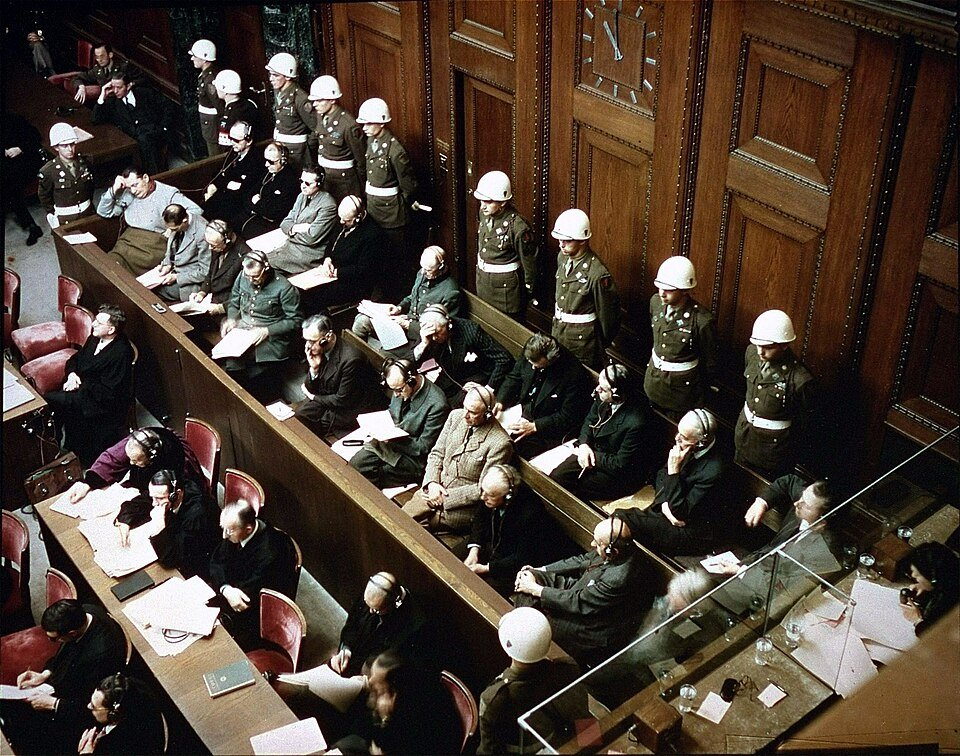
\includegraphics[width=\linewidth]{nuremberg.jpg}\par
      {\scriptsize Նյուրնբերգյան դատավարություն, 1945-1946}
    \end{column}
    \begin{column}{0.5\textwidth}
      \begin{itemize}
        \item Նյուրնբերգում Հոլոքոստի համար պատասխանատուների ամենատարածված պաշտպանությունը
        \item Թույլ արդարացում, չէ՞։ Նորմալ մարդը նման բան չէր անի
      \end{itemize}
      \onslide<2->{%
      \begin{chatbox}
        Գուշակիր. քանի՞ տոկոսը կտա 450 վոլտ «հարված» անծանոթին, եթե գիտնականն ասի։ Գրիր թիվը։
      \end{chatbox}}
    \end{column}
  \end{columns}
\end{frame}

% Milgram's set-up
\begin{frame}{Միլգրամի փորձը}
  \centering
  \begin{tikzpicture}
    \node[personnode, fill=peach!35!cardwhite, text width=2.6cm] (e) at (-3.9,0) {\bigemoji[0.9cm]{scientist}\\ \textbf{Փորձարար}\\ սպիտակ խալաթով};
    \node[personnode, fill=butter!45!cardwhite, text width=2.6cm] (t) at (0.6,0) {\bigemoji[0.9cm]{student}\\ \textbf{«Ուսուցիչ»}\\ իրական մասնակից};
    \draw[plum, dashed, line width=1.2pt] (3.2,-1.3) -- (3.2,1.4);
    \node[font=\scriptsize, text=plum!70!cream, anchor=south] at (3.2,1.4) {պատ};
    \node[personnode, fill=lavender!40!cardwhite, text width=2.6cm, visible on=<2->] (l) at (6.2,0) {\bigemoji[0.9cm]{masks}\\ \textbf{«Աշակերտ»}\\ դերասան};
    \draw[-{Stealth[length=2.6mm]}, plum, line width=1.1pt] (e) -- node[above, font=\small, text=plum] {«Շարունակեք»} (t);
    \draw[-{Stealth[length=2.6mm]}, amRed, line width=1.6pt, visible on=<2->] (t) -- node[below=1mm, font=\blackfont\small, text=amRed, text width=1.9cm, align=center, fill=cream, inner sep=1.5pt] {\emoji{lightning}\ սխալ $\rightarrow$ հարված} (l);
    \begin{scope}[visible on=<3->]
      \foreach \k/\c in {0/mint, 1/butter, 2/peach, 3/blush, 4/amRed}{
        \fill[\c] (-1.6+\k*1.4,-2.0) rectangle ++(1.4,0.42);}
      \draw[plum, line width=0.8pt] (-1.6,-2.0) rectangle ++(7,0.42);
      \node[font=\blackfont\scriptsize, text=plum, anchor=east] at (-1.65,-1.79) {15 Վ};
      \node[font=\blackfont\scriptsize, text=plum, anchor=west] at (5.45,-1.79) {450 Վ};
    \end{scope}
  \end{tikzpicture}\par\vspace{2mm}
  \raggedright
  \onslide<4->{\small Ամեն սխալի համար հարվածն \textbf{ավելի ուժեղ} է։ Բայց հոսանք \textbf{չկար}. դերասանը միտումնավոր սխալվում էր ու ավելի ու ավելի ցավագին ձայներ հանում։\par}
\end{frame}

% The result
\begin{frame}{Արդյունքը}
  \begin{columns}[c]
    \begin{column}{0.36\textwidth}
      \centering
      {\blackfont\fontsize{58}{60}\selectfont\color{amRed} 65\%}\par\smallskip
      {\small գնաց մինչև վերջ՝ 450 Վ (1963)}
    \end{column}
    \begin{column}{0.6\textwidth}
      \begin{itemize}
        \item Մասնակիցները հուզվում էին, առարկում, խնդրում դադարեցնել։ Փորձարարը. «Փորձը կարևոր է, պետք է շարունակել»
        \item<2-> Նրանք բանտերից հավաքված դաժան մարդիկ չէին, այլ \textbf{սովորական} քաղաքացիներ
      \end{itemize}
      \onslide<3->{%
      \begin{bookquote}
        Գուցե առարկում էին, բայց անում էին։ Իսկ հարվածն ստացողի համար հենց \textbf{դա} է կարևոր։
      \end{bookquote}}
    \end{column}
  \end{columns}
\end{frame}

% Variants and today's view
\begin{frame}{Ինչն է փոխում հնազանդությունը}
  \begin{columns}[c]
    \begin{column}{0.54\textwidth}
      \begin{tikzpicture}[x=0.06cm]
        \foreach \y/\v/\l/\t/\c/\s in {0/65/65\%/{առաջին տարբերակը, Յեյլ}/amRed/1,
                                        1/47.5/{47,5\%}/{սովորական գրասենյակ, ոչ Յեյլ}/amBlue/2,
                                        2/22.5/{22,5\%}/{փորձարարը՝ հեռախոսով}/amBlue/2,
                                        3/10/10\%/{երկու «մասնակից» հրաժարվում են}/amBlue/2,
                                        4/43.6/{43,6\%}/{21 տարբերակի միջինը}/amOrange/3}{
          \begin{scope}[visible on=<\s->]
            \node[anchor=south west, font=\small, text=plum, inner sep=1pt] at (0,-\y*0.95+0.3) {\t};
            \fill[\c, rounded corners=1pt] (0,-\y*0.95-0.1) rectangle (\v,-\y*0.95+0.27);
            \node[anchor=west, font=\blackfont\small, text=plum] at (\v,-\y*0.95+0.08) {\l};
          \end{scope}}
      \end{tikzpicture}
    \end{column}
    \begin{column}{0.42\textwidth}
      \onslide<2->{{\small Ապստամբել պատրաստ ենք, բայց \textbf{ոչ առաջինը}։ Սպիտակ խալաթն ու լուրջ գրասենյակը ուժեղացնում են հնազանդությունը։}\par\medskip}
      \onslide<3->{%
      \begin{scienceupdate}
        65\%-ը առաջին տարբերակից է։ 21 տարբերակում (740 մարդ) միջինը \textbf{43,6\%} է։ Ու հարց կա, թե քանիսն էին իսկապես հավատում հարվածներին։
      \end{scienceupdate}}
    \end{column}
  \end{columns}
  \source{Milgram, 1974; Haslam et al., PLoS ONE, 2014; Perry, 2012}
\end{frame}

% Why we obey
\begin{frame}{Ինչու ենք հնազանդվում}
  \begin{columns}[T]
    \begin{column}{0.56\textwidth}
      \begin{itemize}
        \item Հնազանդվում ենք \textbf{օրինական} իշխանությանը, որը պատասխանատու է հետևանքների համար։ Հեռավոր ու արդեն չլսված «պետը» թույլ է
        \item<2-> Միլգրամ. \textbf{ինքնավար} վիճակ (ինքս եմ որոշում) ու \textbf{գործակալային} վիճակ (agentic state, որոշում է ուրիշը)։ Սկաներներում դեռ չի գտնվել
        \item<3-> Էվոլյուցիա. ամեն անգամ «ով է գլխավորը» վիճելը անարդյունավետ է։ Իսկ խարիզմատիկ առաջնորդները դա \textbf{օգտագործում են}
      \end{itemize}
    \end{column}
    \begin{column}{0.4\textwidth}
      \onslide<4->{%
      \begin{card}[colback=peach!35!cardwhite]
        \emoji{judge}\ {\blackfont Էթիկա}\par\smallskip
        Ի՞նչ իրավունք ունեն գիտնականները մարդկանց համոզել, որ նրանք մեկին խոշտանգում են։ Դա կարող է \textbf{ծանր հետք} թողնել։
      \end{card}}
    \end{column}
  \end{columns}
\end{frame}

% Group membership and the self
\begin{frame}{Խումբը՝ «ես»-ի մաս}
  \begin{columns}[c]
    \begin{column}{0.58\textwidth}
      \begin{itemize}
        \item Խմբի մասին մտածելիս ակտիվանում է \textbf{«սոցիալական ուղեղ»} կոչվող ցանցը {\small (չշփոթել նույնանուն \textbf{վարկածի} հետ. գիտնականները շփոթեցնելու առիթ բաց չեն թողնում)}
        \item<2-> Խմբային տեղեկություն մշակող շրջանները \textbf{համընկնում են} «ես»-ը մշակողների հետ
        \item<3-> Ինքնության մեծ մասը գալիս է մեր խմբերից։ Խմբին սպառնալիքը՝ սպառնալիք \textbf{ինձ}
      \end{itemize}
    \end{column}
    \begin{column}{0.38\textwidth}
      \centering
      \begin{tikzpicture}
        \fill[peach!45!cardwhite] (0,0) circle (1.25);
        \fill[lavender!55!cardwhite] (1.4,0) circle (1.25);
        \begin{scope}[visible on=<2->]
          \clip (0,0) circle (1.25);
          \fill[blush!70!cardwhite] (1.4,0) circle (1.25);
        \end{scope}
        \draw[plum, line width=0.9pt] (0,0) circle (1.25) (1.4,0) circle (1.25);
        \node[font=\blackfont, text=plum] at (-0.6,0) {Ես};
        \node[font=\blackfont\small, text=plum] at (2.05,0) {Խումբ};
      \end{tikzpicture}
    \end{column}
  \end{columns}
\end{frame}

% Us and them
\begin{frame}{Մենք ու նրանք}
  \relax{\large Իսկ խմբերին ամենաշատը սպառնում են... \textbf{ուրիշ խմբերը}}\par\medskip
  \begin{columns}[T]
    \begin{column}{0.31\textwidth}
      \begin{card}[colback=peach!35!cardwhite]
        \centering\bigemoji[0.75cm]{trophy}\par\smallskip
        \raggedright Ֆուտբոլային երկրպագուների կռիվները գրեթե \textbf{խաղի շարունակություն} են
      \end{card}
    \end{column}
    \begin{column}{0.31\textwidth}
      \onslide<2->{%
      \begin{card}[colback=butter!45!cream]
        \centering\bigemoji[0.75cm]{ballot}\par\smallskip
        \raggedright Ընտրություններում հակառակորդին հարվածելը ավելի կարևոր է, քան \textbf{ծրագիր} բացատրելը
      \end{card}}
    \end{column}
    \begin{column}{0.31\textwidth}
      \onslide<3->{%
      \begin{card}[colback=lavender!40!cardwhite]
        \centering\bigemoji[0.75cm]{computer}\par\smallskip
        \raggedright Գրիր, որ «Աստղային պատերազմների» նախապատմությունն այդքան էլ վատը չէր։ Մինչև թեյնիկը եռա, փոստդ \textbf{ատելությամբ} կլցվի
      \end{card}}
    \end{column}
  \end{columns}
  \vspace{0.5mm}
  \onslide<3->{\centering\small Բըրնեթը միջազգային կայքի համար բլոգ է գրում. «Վստահեք ինձ այս հարցում»։\par}
\end{frame}

% Stanford prison experiment: the story as the book tells it
\begin{frame}{Ստենֆորդի բանտային փորձը (1971)}
  \begin{columns}[c]
    \begin{column}{0.62\textwidth}
      \begin{itemize}
        \item Ֆիլիպ Զիմբարդոյի թիմը համալսարանի նկուղում բանտ կառուցեց։ Ուսանողներին բաժանեցին «բանտարկյալների» ու «պահակների»
        \item<2-> Պահակները դարձան \textbf{դաժան}. կոպիտ, ագրեսիվ, նվաստացնող։ Բանտարկյալները ապստամբեցին, պահակները ներխուժեցին ու մերկացրին նրանց
        \item<3-> Բանտարկյալների մոտ՝ ընկճվածություն, հեկեկոց, նույնիսկ հոգեծին ցան
        \item<4-> Նախատեսված էր 2 շաբաթ, դադարեցրին \textbf{6 օր} անց
      \end{itemize}
    \end{column}
    \begin{column}{0.34\textwidth}
      \centering
      \bigemoji[1.2cm]{police}\ \bigemoji[1.2cm]{lock}\par\medskip
      \onslide<4->{%
      \begin{card}[colback=peach!35!cardwhite]
        Բըրնեթ. նրանք իրական պահակներ ու բանտարկյալներ չէին, այլ հեղինակավոր համալսարանի \textbf{ուսանողներ}
      \end{card}}
    \end{column}
  \end{columns}
\end{frame}

% Myth or fact: what the SPE proved
\begin{frame}{Առասպել, թե՞ փաստ}
  \mythorfact{Դերը մարդուն դաժանացնում է}{ԿԱՍԿԱԾԵԼԻ Է}{pinkdark}{%
    \begin{scienceupdate}
      Ստենֆորդի պահակներին \textbf{հրահանգել էին} ստեղծել վախի մթնոլորտ (արխիվներ, 2019)։ BBC-ի նման փորձում (2002) պահակները դաժան \textbf{չդարձան}։
    \end{scienceupdate}}
  \source{Le Texier, Am. Psychol., 2019; Reicher \& Haslam, Br. J. Soc. Psychol., 2006}
\end{frame}

% Pecking order
\begin{frame}{Կտցահարման կարգ}
  \begin{columns}[c]
    \begin{column}{0.58\textwidth}
      \begin{itemize}
        \item Դպրոցից ծանոթ է. ինչ-որ մեկը տարօրինակ սանրվածք է անում, «խախտում» է խմբի միօրինակությունը ու \textbf{անվերջ ծաղրվում է}
        \item<2-> Ուզում ենք ոչ միայն խմբում լինել, այլ \textbf{բարձր դիրք} ունենալ։ Նույնիսկ հավերն ունեն հիերարխիա (pecking order)
        \item<3-> Ուղեղի մի քանի շրջաններ (գագաթային ու նախաճակատային կեղևում) հետևում են մեր \textbf{դիրքին} խմբում
        \item<4-> Ծաղրելը նաև սեփական դիրքը \textbf{բարձրացնելու} միջոց է
      \end{itemize}
    \end{column}
    \begin{column}{0.38\textwidth}
      \centering
      \bigemoji[1.3cm]{ladder}\ \bigemoji[1cm]{crown}\par\medskip
      \onslide<4->{\mascot[2cm]{smug}}
    \end{column}
  \end{columns}
\end{frame}

% The group can be anything: country, "race"; cruelty to those in need
\begin{frame}{Խումբը կարող է լինել ամեն ինչ}
  \begin{columns}[T]
    \begin{column}{0.56\textwidth}
      \begin{itemize}
        \item Խումբը կարող է լինել մի ամբողջ \textbf{երկիր}. դա երևում է ամեն դրոշ թափահարողից
        \item<2-> Կամ «ռասա». ֆիզիկական հատկանիշներով հեշտ է տարբերել «օտարին»
        \item<4-> Իսկ հաճախ դաժան ենք նաև նրանց հետ, ովքեր \textbf{օգնության կարիք} ունեն. անօթևաններ, աղքատներ, զոհեր, հիվանդներ, փախստականներ։ Ինչու՞
      \end{itemize}
    \end{column}
    \begin{column}{0.4\textwidth}
      \onslide<3->{%
      \begin{bookquote}
        Ռասիստը այնքան քիչ հպարտանալու բան ունի, որ նրա համար թանկ են ֆիզիկական հատկանիշները, որոնց ձեռքբերման մեջ ինքը \textbf{ոչ մի դեր} չի ունեցել։\par\smallskip
        Զգուշացում. ես ռասիզմի երկրպագու չեմ։
      \end{bookquote}}
    \end{column}
  \end{columns}
\end{frame}

% Egocentric bias and the Singer touch experiment
\begin{frame}{Եսակենտրոն ուղեղ}
  \begin{columns}[T]
    \begin{column}{0.47\textwidth}
      \begin{itemize}
        \item \textbf{Եսակենտրոն շեղում} (egocentric bias). դժվար է ապրումակցել նրանց, ովքեր \textbf{մենք չենք}
        \item Աջ \textbf{վերեզրային գալարը} (supramarginal gyrus) «ուղղում» է շեղումը։ Շտապելիս դա դժվարանում է
      \end{itemize}
    \end{column}
    \begin{column}{0.5\textwidth}
      \onslide<2->{%
      {\small\blackfont Զույգերը դիպչում են հաճելի կամ զզվելի բանի}\par\smallskip
      \begin{tikzpicture}
        \node at (0,0) {\bigemoji[0.75cm]{nauseated}};
        \node at (0.9,0) {\bigemoji[0.75cm]{nauseated}};
        \node[anchor=west, text width=4.3cm, font=\small, text=plum, align=left] at (1.4,0) {Երկուսն էլ \textbf{ճիշտ} են գնահատում իրար};
        \node[visible on=<3->] at (0,-1.15) {\bigemoji[0.75cm]{yum}};
        \node[visible on=<3->] at (0.9,-1.15) {\bigemoji[0.75cm]{nauseated}};
        \node[anchor=west, text width=4.3cm, font=\small, text=plum, align=left, visible on=<3->] at (1.4,-1.15) {Գոհը \textbf{թերագնահատում է} մյուսի տառապանքը};
      \end{tikzpicture}}
    \end{column}
  \end{columns}
  \onslide<4->{%
  \begin{card}[colback=peach!35!cardwhite]
    Որքան հարմարավետ է կյանքդ, այնքան դժվար է հասկանալ նեղության մեջ գտնվողին։ «Քանի դեռ ամենաշփացածներին երկրներ ղեկավարելու չենք դնում, խնդիր չկա»։
  \end{card}}
\end{frame}

% Just-world hypothesis
\begin{frame}{Արդար աշխարհի վարկած (just-world hypothesis)}
  \begin{columns}[c]
    \begin{column}{0.44\textwidth}
      \begin{itemize}
        \item Ուղեղը ենթադրում է, որ աշխարհը \textbf{արդար} է. լավը պարգևատրվում է, վատը՝ պատժվում
        \item Դա օգնում է. զսպում է վատ վարքը ու մոտիվացնում է (թե չէ ինչու՞ վեր կենալ անկողնուց)
        \item<2-> Բայց դա \textbf{ճիշտ չէ}
      \end{itemize}
    \end{column}
    \begin{column}{0.52\textwidth}
      \centering
      \begin{tikzpicture}
        \node[personnode, fill=mint!40!cardwhite, text width=2.5cm] (w) at (-1.6,2.2) {Աշխարհն \textbf{արդար} է};
        \node[personnode, fill=brainpink!30!cardwhite, text width=2.5cm, visible on=<2->] (u) at (1.6,2.2) {Սա \textbf{արդար չէր}};
        \node[personnode, fill=butter!55!cardwhite, visible on=<2->] (d) at (0,0.9) {\emoji{cyclone}\ դիսոնանս};
        \draw[-{Stealth[length=2.5mm]}, plum, line width=1pt, visible on=<2->] (w) -- (d);
        \draw[-{Stealth[length=2.5mm]}, plum, line width=1pt, visible on=<2->] (u) -- (d);
        \node[personnode, text width=3cm, visible on=<3->] (a) at (-1.8,-0.9) {Աշխարհը դաժան է ու \textbf{պատահական}};
        \node[personnode, fill=amRed!15!cardwhite, draw=amRed, line width=1.4pt, text width=3cm, visible on=<4->] (b) at (1.8,-0.9) {\textbf{Զոհն ինքն է} մեղավոր};
        \draw[-{Stealth[length=2.5mm]}, plum, dashed, line width=1pt, visible on=<3->] (d) -- (a);
        \draw[-{Stealth[length=3mm]}, amRed, line width=2pt, visible on=<4->] (d) -- (b);
      \end{tikzpicture}\par\smallskip
      \onslide<4->{{\small Երկրորդն ավելի դաժան է, բայց թույլ է տալիս պահել մեր հարմարավետ (ու սխալ) պատկերացումը}\par}
    \end{column}
  \end{columns}
\end{frame}

% Who do we blame?
\begin{frame}{Ում ենք մեղադրում}
  \begin{itemize}
    \item Զոհին ավելի քիչ են քննադատում, եթե կարող են \textbf{օգնել} նրան, կամ իմանում են, որ նրան փոխհատուցել են։ Եթե օգնել հնարավոր չէ՝ ավելի \textbf{խիստ} են
    \item<2-> Իսկ ավելի շատ մեղադրում ենք նրան, ում հետ \textbf{նույնանում ենք}
  \end{itemize}
  \begin{columns}[T]
    \begin{column}{0.47\textwidth}
      \onslide<2->{%
      \begin{card}[colback=mint!35!cardwhite]
        \emoji{tree}\ Ուրիշ տարիքի ու սեռի մարդու վրա ծառ ընկավ\par\smallskip
        $\rightarrow$ «Խեղճ մարդ, \textbf{պատահականություն} էր»
      \end{card}}
    \end{column}
    \begin{column}{0.47\textwidth}
      \onslide<3->{%
      \begin{card}[colback=brainpink!25!cardwhite]
        \emoji{car}\ Քո տարիքի մարդը քո նման մեքենայով բախվեց քո տան նման տան\par\smallskip
        $\rightarrow$ «\textbf{Ինքն է մեղավոր}, անփույթ էր»
      \end{card}}
    \end{column}
  \end{columns}
  \vspace{2mm}
  \onslide<4->{\centering Որովհետև եթե պատահականություն էր, կարող էր պատահել \textbf{քեզ}։ Իսկ դա վախեցնող միտք է։\par}
\end{frame}

% Chapter conclusion
\begin{frame}{Հրաշալի է}
  \begin{columns}[c]
    \begin{column}{0.58\textwidth}
      \begin{bookquote}
        Չնայած շփման ու ընկերության բոլոր հակումներին, ուղեղը այնքան է մտահոգված իր ինքնության ու հանգստի պահպանմամբ, որ պատրաստ է \textbf{ոտնահարել} ցանկացածին, ով կարող է սպառնալ դրան։\par\smallskip
        Հրաշալի է։
      \end{bookquote}
    \end{column}
    \begin{column}{0.38\textwidth}
      \centering\mascot[3cm]{angry}
    \end{column}
  \end{columns}
\end{frame}

% ===== Wrap-up (~4 min, then questions) =====
\partaccent{butter}\notopic

\begin{frame}{Այսօրվա 5 գաղափարը}
  \begin{enumerate}
    \item<1-> Ուղեղը կառուցված է ուրիշների \textbf{համար} ու ուրիշների \textbf{կողմից}. շփումն անհրաժեշտություն է
    \item<2-> Դեմքը խոսում է, նույնիսկ երբ բառերը լռում են. լիմբիկ համակարգը \textbf{ազնիվ} է
    \item<3-> Ոտքը դռան արանքում, դուռը երեսին, ցածր գնդակ. աշխատում են, որովհետև ուզում ենք, որ մեզ \textbf{սիրեն}
    \item<4-> Բաժանումը ցավում է, որովհետև զուգընկերը դարձել էր քո \textbf{մի մասը}։ Բայց ժամանակը բուժում է
    \item<5-> Խումբը կարող է ստիպել ժխտել սեփական աչքերը, հնազանդվել ու \textbf{մեղադրել զոհին}
  \end{enumerate}
\end{frame}

\begin{frame}{Փորձիր տանը}
  \begin{columns}[T]
    \begin{column}{0.31\textwidth}
      \begin{card}[colback=mint!30!cardwhite]
        \centering\bigemoji[1cm]{tv}\par\smallskip
        \raggedright 5 րոպե ֆիլմ նայիր \textbf{առանց ձայնի}։ Դեմքերից ու ժեստերից որքա՞ն ես հասկանում
      \end{card}
    \end{column}
    \begin{column}{0.31\textwidth}
      \begin{card}[colback=butter!45!cream]
        \centering\bigemoji[1cm]{carrot}\par\smallskip
        \raggedright Հաջորդ «մի փոքր խնդրանքի» կամ «հատուկ առաջարկի» ժամանակ գուշակիր, թե որ \textbf{հնարքն} է
      \end{card}
    \end{column}
    \begin{column}{0.31\textwidth}
      \begin{card}[colback=lavender!35!cardwhite]
        \centering\bigemoji[1cm]{speech}\par\smallskip
        \raggedright Երբ խմբային չաթում մեկն օգնություն է խնդրում, \textbf{մի սպասիր}, որ ուրիշը կպատասխանի
      \end{card}
    \end{column}
  \end{columns}
\end{frame}

\begin{frame}{Հաջորդ վեբինարը}
  \begin{columns}[c]
    \begin{column}{0.6\textwidth}
      \chip[lavender]{brain}{8. Երբ ուղեղը «փչանում» է}\par\medskip
      Շարքի վերջին վեբինարը։ Հոգեկան առողջություն. ինչ է իրականում դեպրեսիան ու ինչ թյուր պատկերացումներ կան դրա մասին, ինչպես է առաջանում «նյարդային պոռթկումը», ինչպես է ուղեղը կախվածություն ձևավորում, և որտեղից են գալիս հալյուցինացիաներն ու զառանցանքները։\par\medskip
      {\small\color{plum!70!cream}Մինչև հիմա տեսանք, թե ինչ տարօրինակ բաներ է անում ուղեղը, երբ \textbf{ամեն ինչ կարգին է}։ Հաջորդ անգամ՝ ինչ է լինում, երբ այն սկսում է խափանվել։}
    \end{column}
    \begin{column}{0.34\textwidth}
      \centering\mascot[2.8cm]{thinking}
    \end{column}
  \end{columns}
\end{frame}

\begin{frame}[plain]
  \begin{tikzpicture}[remember picture, overlay]
    \fill[lavender!60!cream] (current page.south west) rectangle (current page.north east);
    \fill[pattern={Dots[distance=4.4mm, radius=0.28mm]}, pattern color=plum!10!lavender!60!cream]
      (current page.south west) rectangle (current page.north east);
    \node at ([xshift=-3.2cm]current page.center) {\mascot[4.4cm]{happy}};
    \node[anchor=west, text=plum] at ([xshift=0.2cm, yshift=0.6cm]current page.center)
      {\titlefont\fontsize{40}{42}\selectfont Հարցեր};
    \node[anchor=west, text=plum, font=\mediumfont\large, align=left] at ([xshift=0.2cm, yshift=-1.0cm]current page.center)
      {Գրեք չաթում կամ\\ միացրեք խոսափողը \emoji{megaphone}};
    \node[anchor=west, text=plum!70!cream, font=\small] at ([xshift=0.2cm, yshift=-2.1cm]current page.center)
      {Դին Բըրնեթ, «The Idiot Brain», 2016};
  \end{tikzpicture}
\end{frame}

% ===== Appendix: corrections to the book, what we added, sources (after Questions; not presented) =====
\appendix
\partaccent{lavender}\gdef\idiottopicemoji{books}\gdef\idiottopicname{Հավելված}
\newcolumntype{L}[1]{>{\raggedright\arraybackslash}p{#1}}

\begin{frame}{Հավելված Ա. Ուղղումներ գրքի նկատմամբ (1/2)}
  \scriptsize
  \setlength{\tabcolsep}{4pt}
  \renewcommand{\arraystretch}{1.3}
  \begin{tabular}{@{}L{2.3cm}L{3.3cm}L{4.6cm}L{3.3cm}@{}}
    \toprule
    \textbf{Թեմա} & \textbf{Գրքում (2016)} & \textbf{Այսօր} & \textbf{Աղբյուր}\\
    \midrule
    Աշի փորձը & «75\% դեպքերում սխալ էին»; «որն է ամենաերկարը» & Սխալները մոտ 37\% էին, 75\%-ը սխալվել է գոնե մեկ անգամ։ Հարցը՝ որն է նույն երկարությամբ & Asch, Psychol. Monogr., 1956\\
    Միլգրամ & 65\%-ը գնաց մինչև վերջ & Առաջին տարբերակում՝ այո։ 21 տարբերակի միջինը 43,6\% է & Haslam et al., PLoS ONE, 2014; Perry, 2012\\
    Ստենֆորդի բանտ & Պահակներն իրենք դարձան դաժան & Նրանց հրահանգել էին։ BBC-ի նման փորձում չկրկնվեց & Le Texier, Am. Psychol., 2019; Reicher \& Haslam, 2006\\
    Ամբոխ & Կորցնում ենք անհատականությունը & Ավելի խիստ հետևում ենք խմբի նորմերին & Postmes \& Spears, Psychol. Bull., 1998\\
    Դիտորդի էֆեկտ & 38 անտարբեր վկա (գիրքն ինքն է նշում չափազանցությունը) & Իրական կոնֆլիկտների 91\%-ում գոնե մեկն օգնում է & Philpot et al., Am. Psychol., 2020\\
    \bottomrule
  \end{tabular}
\end{frame}

\begin{frame}{Հավելված Ա. Ուղղումներ գրքի նկատմամբ (2/2)}
  \scriptsize
  \setlength{\tabcolsep}{4pt}
  \renewcommand{\arraystretch}{1.3}
  \begin{tabular}{@{}L{2.3cm}L{3.3cm}L{4.6cm}L{3.3cm}@{}}
    \toprule
    \textbf{Թեմա} & \textbf{Գրքում (2016)} & \textbf{Այսօր} & \textbf{Աղբյուր}\\
    \midrule
    Դիմախաղ & Բնածին է ու համընդհանուր & Վիճելի է. ազատ դասավորման դեպքում հեռավոր մշակույթը այլ կերպ է խմբավորում & Gendron et al., Emotion, 2014; Barrett et al., 2019\\
    Օքսիտոցին & Կապված է վստահության հետ & Քթի սփրեյով փորձերը լավ չեն կրկնվում & Nave et al., Perspect. Psychol. Sci., 2015\\
    Բաժանում ու ցավ & Նույն շրջանները, ինչ ֆիզիկական ցավը & Մասամբ համընկնում են, բայց ակտիվության նախշերը տարբեր են & Woo et al., Nat. Commun., 2014\\
    Սոցիալական ուղեղ & Մեծ ուղեղը՝ սոցիալական կյանքից & Պրիմատների մոտ սննդակարգն ավելի լավ է կանխատեսում ուղեղի չափը. վեճը բաց է & DeCasien et al., Nat. Ecol. Evol., 2017\\
    Ցածր գնդակ & Նախ համաձայնել էին ժամը 9-ին & Սկզբում ժամը չէին ասում (56\% ընդդեմ 31\%) & Cialdini et al., JPSP, 1978\\
    Դուռը երեսին & «Ուսանողներ» & 6-8 տարեկան երեխաներ & Chan \& Au, 2011\\
    \bottomrule
  \end{tabular}
\end{frame}

\begin{frame}{Հավելված Բ. Ինչ ենք ավելացրել գրքից դուրս}
  \begin{columns}[T]
    \begin{column}{0.48\textwidth}
      \begin{card}[colback=mint!30!cardwhite, fontupper=\scriptsize]
        {\blackfont Թվեր ու հետազոտություններ}\par\smallskip
        \begin{itemize}\setlength{\itemsep}{0.5mm}
          \item Մենախցի սահմանումը՝ ՄԱԿ-ի Նելսոն Մանդելայի կանոններ, 2015
          \item «7-38-55»՝ Mehrabian \& Wiener, 1967
          \item Երեխաների տարիքը՝ Chan \& Au, 2011
          \item Ժամը 7-ի փորձի թվերը՝ Cialdini et al., 1978
          \item Աշի թվերը՝ Asch, 1956
          \item Դիտորդի էֆեկտի թվերը՝ Darley \& Latané, 1968
          \item Միլգրամի տարբերակները՝ Milgram, 1974
          \item «Գիտությունն այսօր» տուփերը (ուղղումների աղյուսակում)
        \end{itemize}
      \end{card}
    \end{column}
    \begin{column}{0.48\textwidth}
      \begin{card}[colback=peach!35!cardwhite, fontupper=\scriptsize]
        {\blackfont Մերն է, ոչ թե գրքից}\par\smallskip
        \begin{itemize}\setlength{\itemsep}{0.5mm}
          \item Աֆազիաների հայերեն օրինակները (գրքում՝ անգլերեն)
          \item «Պետք չէր»-ի, էմոտիկոնների ու Աշի չաթային «փորձերը»
          \item Գումարները դրամով (գրքում՝ ֆունտով)
          \item Լեզվի շրջանների նկարը (Wikimedia Commons, հանրային սեփականություն), սիրամարգի ու Նյուրնբերգի լուսանկարները (Wikimedia Commons)
          \item Մեմերը. բովանդակությունը գրքից է
        \end{itemize}
      \end{card}
    \end{column}
  \end{columns}
\end{frame}

\begin{frame}{Հավելված Գ. Աղբյուրներ (1/2)}
  \scriptsize
  Գրքի ծանոթագրություններից, որոնց վրա հիմնված են սլայդները\par\smallskip
  \begin{columns}[T]
    \begin{column}{0.48\textwidth}
      \begin{itemize}\setlength{\itemsep}{0.4mm}
        \item Conley A. Torture in US jails and prisons. Vienna J. Int. Const. Law, 2013
        \item Pasley B. N. et al. Reconstructing speech from human auditory cortex. PLoS Biol., 2012
        \item Lucy J. A. Language Diversity and Thought. 1992
        \item Davies I. R. A study of colour grouping in three languages. Br. J. Psychol., 1998
        \item Sacks O. The Man Who Mistook His Wife for a Hat. 1985
        \item Whalen P. J. et al. Neuroscience and facial expressions of emotion. Emotion Rev., 2013
        \item Guéguen N. Foot-in-the-door technique and computer-mediated communication. Comput. Hum. Behav., 2002
      \end{itemize}
    \end{column}
    \begin{column}{0.48\textwidth}
      \begin{itemize}\setlength{\itemsep}{0.4mm}
        \item Chan A. C., Au T. K. Getting children to do more academic work. Teach. Teach. Educ., 2011
        \item Ebster C., Neumayr B. Applying the door-in-the-face technique to retailing. 2008
        \item Burger J. M., Cornelius T. Raising the price of agreement. J. Appl. Soc. Psychol., 2003
        \item Cialdini R. B. et al. Low-ball procedure for producing compliance. JPSP, 1978
        \item Farrow T. F. et al. Neural correlates of self-deception and impression-management. Neuropsychologia, 2015
        \item Coxworth J. E. et al. Grandmothering life histories and human pair bonding. PNAS, 2015
        \item Aron A. et al. Reward, motivation, and emotion systems in early-stage romantic love. J. Neurophysiol., 2005
      \end{itemize}
    \end{column}
  \end{columns}
\end{frame}

\begin{frame}{Հավելված Դ. Աղբյուրներ (2/2)}
  \scriptsize
  Գրքի ծանոթագրություններից, որոնց վրա հիմնված են սլայդները\par\smallskip
  \begin{columns}[T]
    \begin{column}{0.48\textwidth}
      \begin{itemize}\setlength{\itemsep}{0.4mm}
        \item Hays W. S. Human pheromones: have they been demonstrated? Behav. Ecol. Sociobiol., 2003
        \item Kross E. et al. Social rejection shares somatosensory representations with physical pain. PNAS, 2011
        \item Fisher H. E. et al. Reward, addiction, and emotion regulation systems associated with rejection in love. J. Neurophysiol., 2010
        \item Dunbar R. I. The social brain hypothesis and its implications. Ann. Hum. Biol., 2009
        \item Dávid-Barrett T., Dunbar R. Processing power limits social group size. Proc. R. Soc. B, 2013
        \item Asch S. E. Studies of independence and conformity. Psychol. Monogr., 1956
        \item Latané B., Darley J. M. Bystander «apathy». Am. Sci., 1969
      \end{itemize}
    \end{column}
    \begin{column}{0.48\textwidth}
      \begin{itemize}\setlength{\itemsep}{0.4mm}
        \item Janis I. L. Groupthink. 1982
        \item Reicher S. D., Spears R., Postmes T. A social identity model of deindividuation phenomena. Eur. Rev. Soc. Psychol., 1995
        \item Milgram S. Behavioral study of obedience. J. Abnorm. Soc. Psychol., 1963
        \item Morrison S., Decety J., Molenberghs P. The neuroscience of group membership. Neuropsychologia, 2012
        \item Zimbardo P. G. Stanford Prison Experiment. 1971
        \item Silani G. et al. Right supramarginal gyrus is crucial to overcome emotional egocentricity bias. J. Neurosci., 2013
        \item Strömwall L. A. et al. Victim blame and the just world hypothesis. J. Sex. Aggress., 2013
      \end{itemize}
    \end{column}
  \end{columns}
\end{frame}

\end{document}
